\chapter{Phonology}\label{section phono}
In this chapter we present the basic segmental inventory  (\S\ref{section:phono:segmental}) and suprasegmental phonology (\S\ref{section:phono:suprasegmental})  of  {\iaIA}.\largerpage




\section{Segmental phonology}\label{section:phono:segmental}
\begin{sloppypar}
Table \ref{table: consontants of iranian} lists the consonant inventory of {\iaIA}, including both phonemes and non-contrastive sounds in parentheses.
\end{sloppypar}

	\begin{table}
	
	\caption{Consonant inventory of {\iaIA}}\label{table: consontants of iranian}
	\centering
	\begin{tabular}{l  ll  l lll ll  l}
		\lsptoprule
		&\multicolumn{2}{c}{Labial}	&\multicolumn{4}{c}{Coronal} &\multicolumn{3}{c}{Dorsal/Back}\\\cmidrule(lr){2-3}\cmidrule(lr){4-7}\cmidrule(lr){8-10}
		Stop
		&
		{p} &  b& {t} &  d  &&  &   {k} &  ɡ & 
		\\
		& pʰ & & tʰ & & & & kʰ & & 
		\\
		
		Affricate &   & & {t͡s} &   d͡z&  {t͡ʃ}     &d͡ʒ &&  & \\
		&&  & t͡sʰ & & t͡ʃʰ  & & && \\
		Nasal & &{m}&  & {n} & &&&  (ŋ) &	\\
		Fricative & {f} & v & {s}& z&  {ʃ} & ʒ & {χ}  & ʁ& {h}\\
		Liquid  && & & {ɻ} &   & {l} & & & \\
		&& & &   {r} &  & & & & \\
		Glide & &&&   {j} &  &&&    ({w})  &  \\ \lspbottomrule
	\end{tabular}
	
	
\end{table}



{\iaIA} has largely the same phonemic inventory as   {\seaEA}. For example, both utilize a three-way laryngeal contrast for stops and affricates: D, T, Tʰ  (\S\ref{section:phono:segmental:laryngeal cons}).  General overviews of {\seaSEA} segmental phonology are found in \citet[\S1]{Vaux-1998-ArmenianPhono} and \citet[\S1--3]{Johnson-1954-EastArmGrammar}.



The lects do differ in a few   aspects. In terms of rhotics (\S\ref{section:phono:segmental:rhotic}), Eastern has a phonemic trill /{r}/ and phonemic flap /{ɾ}/, while {\iaIA} has a phonemic trill /r/ and phonemic approximant /{ɻ}/. 

Both dialects have [ŋ] as a non-phonemic allophone of /n/ before velar stops. {\iaIA} utilizes a glide [{w}] as a non-contrastive epenthetic segment, while this segment is absent for {\seaSE} (\S\ref{section:phono:segmental:other cons}). We show these two sounds with parentheses in Table \ref{table: consontants of iranian}.  







In terms of vowels (\S\ref{section:phono:segmental:vowel}) in Figure \ref{fig: vowel inventory}, the low back vowel is unrounded /{ɑ}/ in {\seaSE} but rounded /{ɒ}/ in {\iaIA}. {\iaIA} also has a  low front vowel /{æ}/ as a marginal phoneme. 


\begin{figure}[H]
	
	\centering
	\caption{Vowel inventory of {\iaIA} }
	\label{fig: vowel inventory}
	\begin{tikzpicture}[scale=3]
		\large
		\tikzset{
			vowel/.style={fill=white, anchor=mid, text depth=0ex, text height=1ex},
			dot/.style={circle,fill=black,minimum size=0.4ex,inner sep=0pt,outer sep=-1pt},
		}
		\coordinate (hf) at (0,2); % high front
		\coordinate (hb) at (2,2); % high back
		\coordinate (lf) at (1,0); % low front
		\coordinate (lb) at (2,0); % low back
		\def\V(#1,#2){barycentric cs:hf={(3-#1)*(2-#2)},hb={(3-#1)*#2},lf={#1*(2-#2)},lb={#1*#2}}
		
		% Draw the horizontal lines first.
		\draw (\V(0,0)) -- (\V(0,2));
		\draw (\V(1,0)) -- (\V(1,2));
		\draw (\V(2,0)) -- (\V(2,2));
		% \draw (\V(3,0)) -- (\V(3,2));
		
		% Place all the unrounded-rounded pairs next, on top of the horizontal lines.
		\path (\V(0,0))     node[vowel, left] {i}   node[dot] {};
		% \path (\V(0,1))     node[vowel, left] {ɨ} node[vowel, right] {ʉ} node[dot] {};
		\path (\V(0,2))     node[vowel, right] {u} node[dot] {};
		% \path (\V(0.5,0.4)) node[vowel, left] {ɪ} node[vowel, right] {ʏ} node[dot] {};
		% \path (\V(0.5,1.6)) node[vowel, left] { } node[vowel, right] {ʊ} node[dot] {};
		\path (\V(1,0))     node[vowel, left] {e}    {};
		\path (\V(1,2))       node[vowel, right] {o} node[dot] {};
		\path (\V(2,0))     node[vowel, left] {æ}   node[dot] {};
		% \path (\V(2,1))     node[vowel, left] {ɜ} node[vowel, right] {ɞ} node[dot] {};
		\path (\V(2,2))     node[vowel, right] {{ɒ}} node[dot] {};
		% \path (\V(2.5,0))   node[vowel, left] {æ} node[vowel, right] { } node[   ] {};
		% \path (\V(3,0))     node[vowel, left] {a} node[vowel, right] {ɶ} node[dot] {};
		% \path (\V(3,2))     node[vowel, right] {ɒ} node[dot] {};
		
		% Draw the vertical lines.
		\draw (\V(0,0)) -- (\V(2,0));
		\draw (\V(0,1)) -- (\V(2,1));
		\draw (\V(0,2)) -- (\V(2,2));
		
		% Place the unpaired symbols last, on top of the vertical lines.
		% \path (\V(1.5,1))   node[vowel]       {ə};
		\path (\V(1,1))     node[vowel] {ə}     ;
		% \path (\V(2.5,1))   node[vowel]       {ɐ};
	\end{tikzpicture}
	
	
\end{figure}



%\begin{figure}
%	
%	\caption{Consonant and vowel inventory of {\iaIA} }
%	\label{fig:cons vowel inventory}
%	\begin{subfigure}[b]{0.5\textwidth}
	%		\centering
	%		\caption{Consonant inventory }\label{table: consontants of iranian}
	%		\begin{tabular}{|l|  l| ll| ll|}
		%			\hline 		&Labial	&\multicolumn{2}{l|}{Coronal}
		%			&\multicolumn{2}{l|}{Dorsal}
		%			\\ 
		%			Stop
		%			&
		%			{p} & {t}  & &  {k} & 
		%			\\
		%			& {pʰ}  & {tʰ}  & &  {kʰ} &
		%			\\
		%			& {b} & {d} & &  {ɡ} &
		%			\\
		%			
		%			Affricate & & {t͡s} & {t͡ʃ} & & 
		%			\\
		%			& & {t͡sʰ} & {t͡ʃʰ} & & 
		%			\\
		%			& & {d͡z}& {d͡ʒ}& &
		%			\\
		%			Nasal
		%			& {m} & {n} & &(ŋ) & 
		%			\\
		%			Fricative & {f} & {s} & {ʃ} & {χ} & {h}
		%			\\
		%			& {v} & {z} & {ʒ} & {ʁ}   & 
		%			\\
		%			Liquid  && {ɻ} & {r} & {l} &
		%			\\
		%			Glide & & {j} &  &({w})  &  
		%			\\ \hline
		%		\end{tabular}
	%		
	%	\end{subfigure}
%	\hspace{3cm}
%	\begin{subfigure}[b]{0.5\textwidth}
	%		\centering
	%		\caption{Vowel inventory }
	%		\label{fig: vowel inventory}
	%		\begin{tikzpicture}[scale=3]
		%			\large
		%			\tikzset{
			%				vowel/.style={fill=white, anchor=mid, text depth=0ex, text height=1ex},
			%				dot/.style={circle,fill=black,minimum size=0.4ex,inner sep=0pt,outer sep=-1pt},
			%			}
		%			\coordinate (hf) at (0,2); % high front
		%			\coordinate (hb) at (2,2); % high back
		%			\coordinate (lf) at (1,0); % low front
		%			\coordinate (lb) at (2,0); % low back
		%			\def\V(#1,#2){barycentric cs:hf={(3-#1)*(2-#2)},hb={(3-#1)*#2},lf={#1*(2-#2)},lb={#1*#2}}
		%			
		%			% Draw the horizontal lines first.
		%			\draw (\V(0,0)) -- (\V(0,2));
		%			\draw (\V(1,0)) -- (\V(1,2));
		%			\draw (\V(2,0)) -- (\V(2,2));
		%			% \draw (\V(3,0)) -- (\V(3,2));
		%			
		%			% Place all the unrounded-rounded pairs next, on top of the horizontal lines.
		%			\path (\V(0,0))     node[vowel, left] {i}   node[dot] {};
		%			% \path (\V(0,1))     node[vowel, left] {ɨ} node[vowel, right] {ʉ} node[dot] {};
		%			\path (\V(0,2))     node[vowel, right] {u} node[dot] {};
		%			% \path (\V(0.5,0.4)) node[vowel, left] {ɪ} node[vowel, right] {ʏ} node[dot] {};
		%			% \path (\V(0.5,1.6)) node[vowel, left] { } node[vowel, right] {ʊ} node[dot] {};
		%			\path (\V(1,0))     node[vowel, left] {e}    {};
		%			\path (\V(1,2))       node[vowel, right] {o} node[dot] {};
		%			\path (\V(2,0))     node[vowel, left] {æ}   node[dot] {};
		%			% \path (\V(2,1))     node[vowel, left] {ɜ} node[vowel, right] {ɞ} node[dot] {};
		%			\path (\V(2,2))     node[vowel, right] {{ɒ}} node[dot] {};
		%			% \path (\V(2.5,0))   node[vowel, left] {æ} node[vowel, right] { } node[   ] {};
		%			% \path (\V(3,0))     node[vowel, left] {a} node[vowel, right] {ɶ} node[dot] {};
		%			% \path (\V(3,2))     node[vowel, right] {ɒ} node[dot] {};
		%			
		%			% Draw the vertical lines.
		%			\draw (\V(0,0)) -- (\V(2,0));
		%			\draw (\V(0,1)) -- (\V(2,1));
		%			\draw (\V(0,2)) -- (\V(2,2));
		%			
		%			% Place the unpaired symbols last, on top of the vertical lines.
		%			% \path (\V(1.5,1))   node[vowel]       {ə};
		%			\path (\V(1,1))     node[vowel] {ə}     ;
		%			% \path (\V(2.5,1))   node[vowel]       {ɐ};
		%		\end{tikzpicture}
	%		
	%	\end{subfigure}
%\end{figure}



\subsection{Laryngeal qualities of consonants}\label{section:phono:segmental:laryngeal cons}

Both {\seaSE} and {\iaIA}  utilize a three-way laryngeal contrast for stops and affricates based on voice onset time (VOT). There is a phonemic contrast between prevoiced or voiced (-VOT), voiceless unaspirated (0VOT), and voiceless aspirated (+VOT) consonants. We provide near-minimal pairs in Table \ref{tab:stops affricates} from {\iaIA}.  In general, there is a separate grapheme (orthographic letter) for each type of phonemic stop/affricate. We list the graphemes in the first column, and the phonemes in the second column.

Acoustic data on the three-way contrast can be found for both {\iaIA} \citep{Hacopian-2003-ThreeWayVOTCOntrastArmenian,Amirian-2017-TehraniStudyAcousticFeaturesStopsAffricatesEasternArmenian,Toparlak-2017-MAConsonantsArmenian}  and {\seaSE} \citep{Seyfarth-2018-PlosiveVoicingAcousticsArmenian,Seyfarth-JIPAArmenian}. The contrast is maintained even word-finally. However, there are very few words that are pronounced with word-final voiced obstruents.  The coronals have been reported to be dental in {\seaSE} \citep[110]{Khachatryan-1988-ArmenianPhono}, but we are unsure if they are also dental in {\iaIA}.\footnote{NK self-reported a dental articulation for some tokens with initial coronal stops, but also reported alveolar articulation for other tokens.} 



\begin{table}
	\caption{three-way laryngeal contrast for stops and affricates\label{tab:stops affricates}}
% 	\resizebox{\textwidth}{!}{%
\small
\tabcolsep=.66\tabcolsep
		\begin{tabular}{ll ll ll ll}
			\lsptoprule 
			& &\multicolumn{2}{c}{Initial}&\multicolumn{2}{c}{Medial}&\multicolumn{2}{c}{Final}\\\cmidrule(lr){3-4}\cmidrule(lr){5-6}\cmidrule(lr){7-8}
				\armenian{բ} & /{b}/ 
			& {ˈ\textbf{b}ɒr} &`word' 
			& {ɒɻɒ\textbf{b}eˈɻen} & `Arabic' 
			& {æˈɻæ\textbf{b}} & `Arab' 
			\\
			& 
			&  &  \armenian{բառ}
			&  & \armenian{արաբերէն}
			&   & \armenian{արաբ}
			\\ 
			
			\armenian{պ} & /{p}/ & {\textbf{p}ɒˈniɻ}&`cheese'  & {ɒ\textbf{p}ɒˈki}   &`glass'
			& {ˈkɒ\textbf{p}}   &`connection'
			\\
			& &  &\armenian{պանիր}&     &\armenian{ապակի}
			&    &\armenian{կապ}
			
			\\
			\armenian{փ}
			&/{pʰ}/&{ˈ\textbf{pʰ}iʁ}&`elephant'
			&{t͡ʃʰɒˈ\textbf{pʰ}el}&`to measure'
			&{ˈtu\textbf{pʰ}}&`box'
			\\
			& & &\armenian{փիղ}
			& &\armenian{չափել}
			& &\armenian{տուփ}
			\\
		\midrule 
						\armenian{դ} & /{d}/
			& {ˈ\textbf{d}ɒɻ} & `century' 
			& {bɒˈ\textbf{d}ik} & `duckling' 
			&{ˈbɒ\textbf{d} } &`duck' \\
			&  
			&   & \armenian{դար}
			&   & \armenian{բադիկ}
			&& \armenian{բադ}\\
			
			\armenian{տ} & /{t}/ 
			& {ˈ\textbf{t}un} &`house' 
			& {pʰeˈ\textbf{t}uɻ} &`feather' 
			& {ˈsu\textbf{t}} & `lie' 
			\\
			&  
			&   &  \armenian{տուն}
			&   & \armenian{փետուր}
			&   & \armenian{սուտ}
			\\
			\armenian{թ} & /{tʰ}/ 
			& {ˈ\textbf{tʰ}uɻkʰ} & `Turk' 
			& {d͡ʒuˈ\textbf{tʰ}ɒk} &  `violin'
			& {ˈkɒ\textbf{tʰ}} &`milk'
			\\
			&  
			&   &   \armenian{թուրք}
			&   & \armenian{ջութակ}
			& &     \armenian{կաթ}
			\\
	\midrule 
			\armenian{գ} & /{ɡ}/ 
		& {ˈ\textbf{ɡ}iɻkʰ} &`book'  
		& {ɒˈɻɒ\textbf{ɡ}-ə} &  `fast-{\defgloss}'
		& {ˈtʰɒ\textbf{ɡ}} &  `crown'
		\\
		&  &   & \armenian{գիրք}
		&   & \armenian{արագը}
		&  &  \armenian{թագ}
		\\
			\armenian{կ} & /{k}/ 
			& {\textbf{k}ɒɻˈtʰɒl} & `to read'
			& {t͡ʃɒˈ\textbf{k}ɒt} & `forehead'
			& {ˈbɒ\textbf{k}} & `yard'
			\\
			&  
			&   & \armenian{կարդալ}
			&  & \armenian{ճակատ}
			&   & \armenian{բակ}
			\\
			\armenian{ք} & /{kʰ}/ 
			& {ˈ\textbf{kʰ}ɒɻ} & `rock' 
			&{mɒˈ\textbf{kʰ}uɻ} & `clean'
			&{kʰɒˈʁɒ\textbf{kʰ}} & `city'
			\\
			&  
			& & \armenian{քար}
			&  & \armenian{մաքուր}
			&  & \armenian{քաղաք}
			\\
			\midrule 
			\armenian{ձ} & /{d͡z}/ 
		& {ˈ\textbf{d͡z}un}& `snow' 
		& {hɒmɒ\textbf{ˈd͡z}ɒjn}   &  `agreeing' 
		& {ˈin\textbf{d͡z}} &  `me.{\dat}'
		\\
		&  
		& & \armenian{ձուն}
		&   &\armenian{համաձայն}
		& &\armenian{ինձ}
		\\
			\armenian{ծ} &/{t͡s}/ 
			&  {ˈ\textbf{t͡s}ɒr}& `tree' 
			& {kəˈ\textbf{t͡s}u} &`spicy'
			& {ˈme\textbf{t͡s}} &`big'
			\\
			& 
			& &  \armenian{ծառ}
			& &  \armenian{կծու}
			&  &   \armenian{մեծ}
			\\
			\armenian{ց} & /{t͡sʰ}/ 
			& {ˈ\textbf{t͡sʰ}ɒv} & `pain'
			& {hɒˈ\textbf{t͡sʰ}-i} &`bread-{\gen}'
			& {ˈbɒ\textbf{t͡sʰ}} &   `open'
			\\
			&  
			& &  \armenian{ցաւ}
			& &   \armenian{հացի}
			&  & \armenian{բաց}
			\\
			\midrule 
		\armenian{ջ} & /{d͡ʒ}/
	& {ˈ\textbf{d͡ʒ}uɻ} &`water' 
	& {d͡ʒənˈ\textbf{d͡ʒ}ik} &`eraser'
	& {ˈkʰɒ\textbf{d͡ʒ}} &`brave'
	
	\\ 
			& &
		&  \armenian{ջուր}
		&    &  \armenian{ջնջիկ}
		&   &  \armenian{քաջ}
		
		\\ 
			\armenian{ճ} & /{t͡ʃ}/ 
			& {\textbf{t͡ʃ}ɒˈɻel} & `to look for' 
			& {ɒˈ\textbf{t͡ʃ}el} &  `to grow'
			& {ˈli\textbf{t͡ʃ}} & `lake'
			\\
			&  
			& & \armenian{ճարել}
			&   &\armenian{աճել}
			&  &  \armenian{լիճ}
			\\
			\armenian{չ} & /{t͡ʃʰ}/ 
			& {ˈ\textbf{t͡ʃʰ}ɒɻ} &  `evil'
			& {ɒˈ\textbf{t͡ʃʰ}-it͡sʰ} &`right-{\abl}'
			& {ˈvo\textbf{t͡ʃʰ}} &  `no'
			\\
			&   
			& & \armenian{չար}
			&  &  \armenian{աջից}
			&   &  \armenian{ոչ}
			\\
			\lspbottomrule 
		\end{tabular}
% 		}
\end{table}









For word-final voiceless unaspirated stops ({p, t, k}), it is reported that some {\iaIA} speakers pronounce these sounds as ejectives  \citep{fleming-2000-GlottalizationEasternArmenian,Toparlak-2017-MAConsonantsArmenian,ToparlakDolatian-2023-AerodynamicsarticulationwordfinalejectivesEasternArmenian}, while some do not \citep{Amirian-2017-TehraniStudyAcousticFeaturesStopsAffricatesEasternArmenian}. For NK, we rarely heard any ejectivized tokens. Figure \ref{fig:ejective} shows an example of a final ejectivized unaspirated /{k}/, along with an un-ejectivized one. The recordings for these two words can be found in our online archive.\footnote{\url{https://github.com/jhdeov/iranian_armenian}}
  There is a larger debate about whether any varieties of modern or ancient Armenian possess(ed) a glottalized or ejective series of voiceless stops; for discussion and references see \citet{Vaux-2022-EjectiveSlides}.

\begin{figure}
	\caption{Variable ejectivization of final unaspirated stops from NK\label{fig:ejective}}
	\begin{subfigure}[b]{0.5\textwidth}
		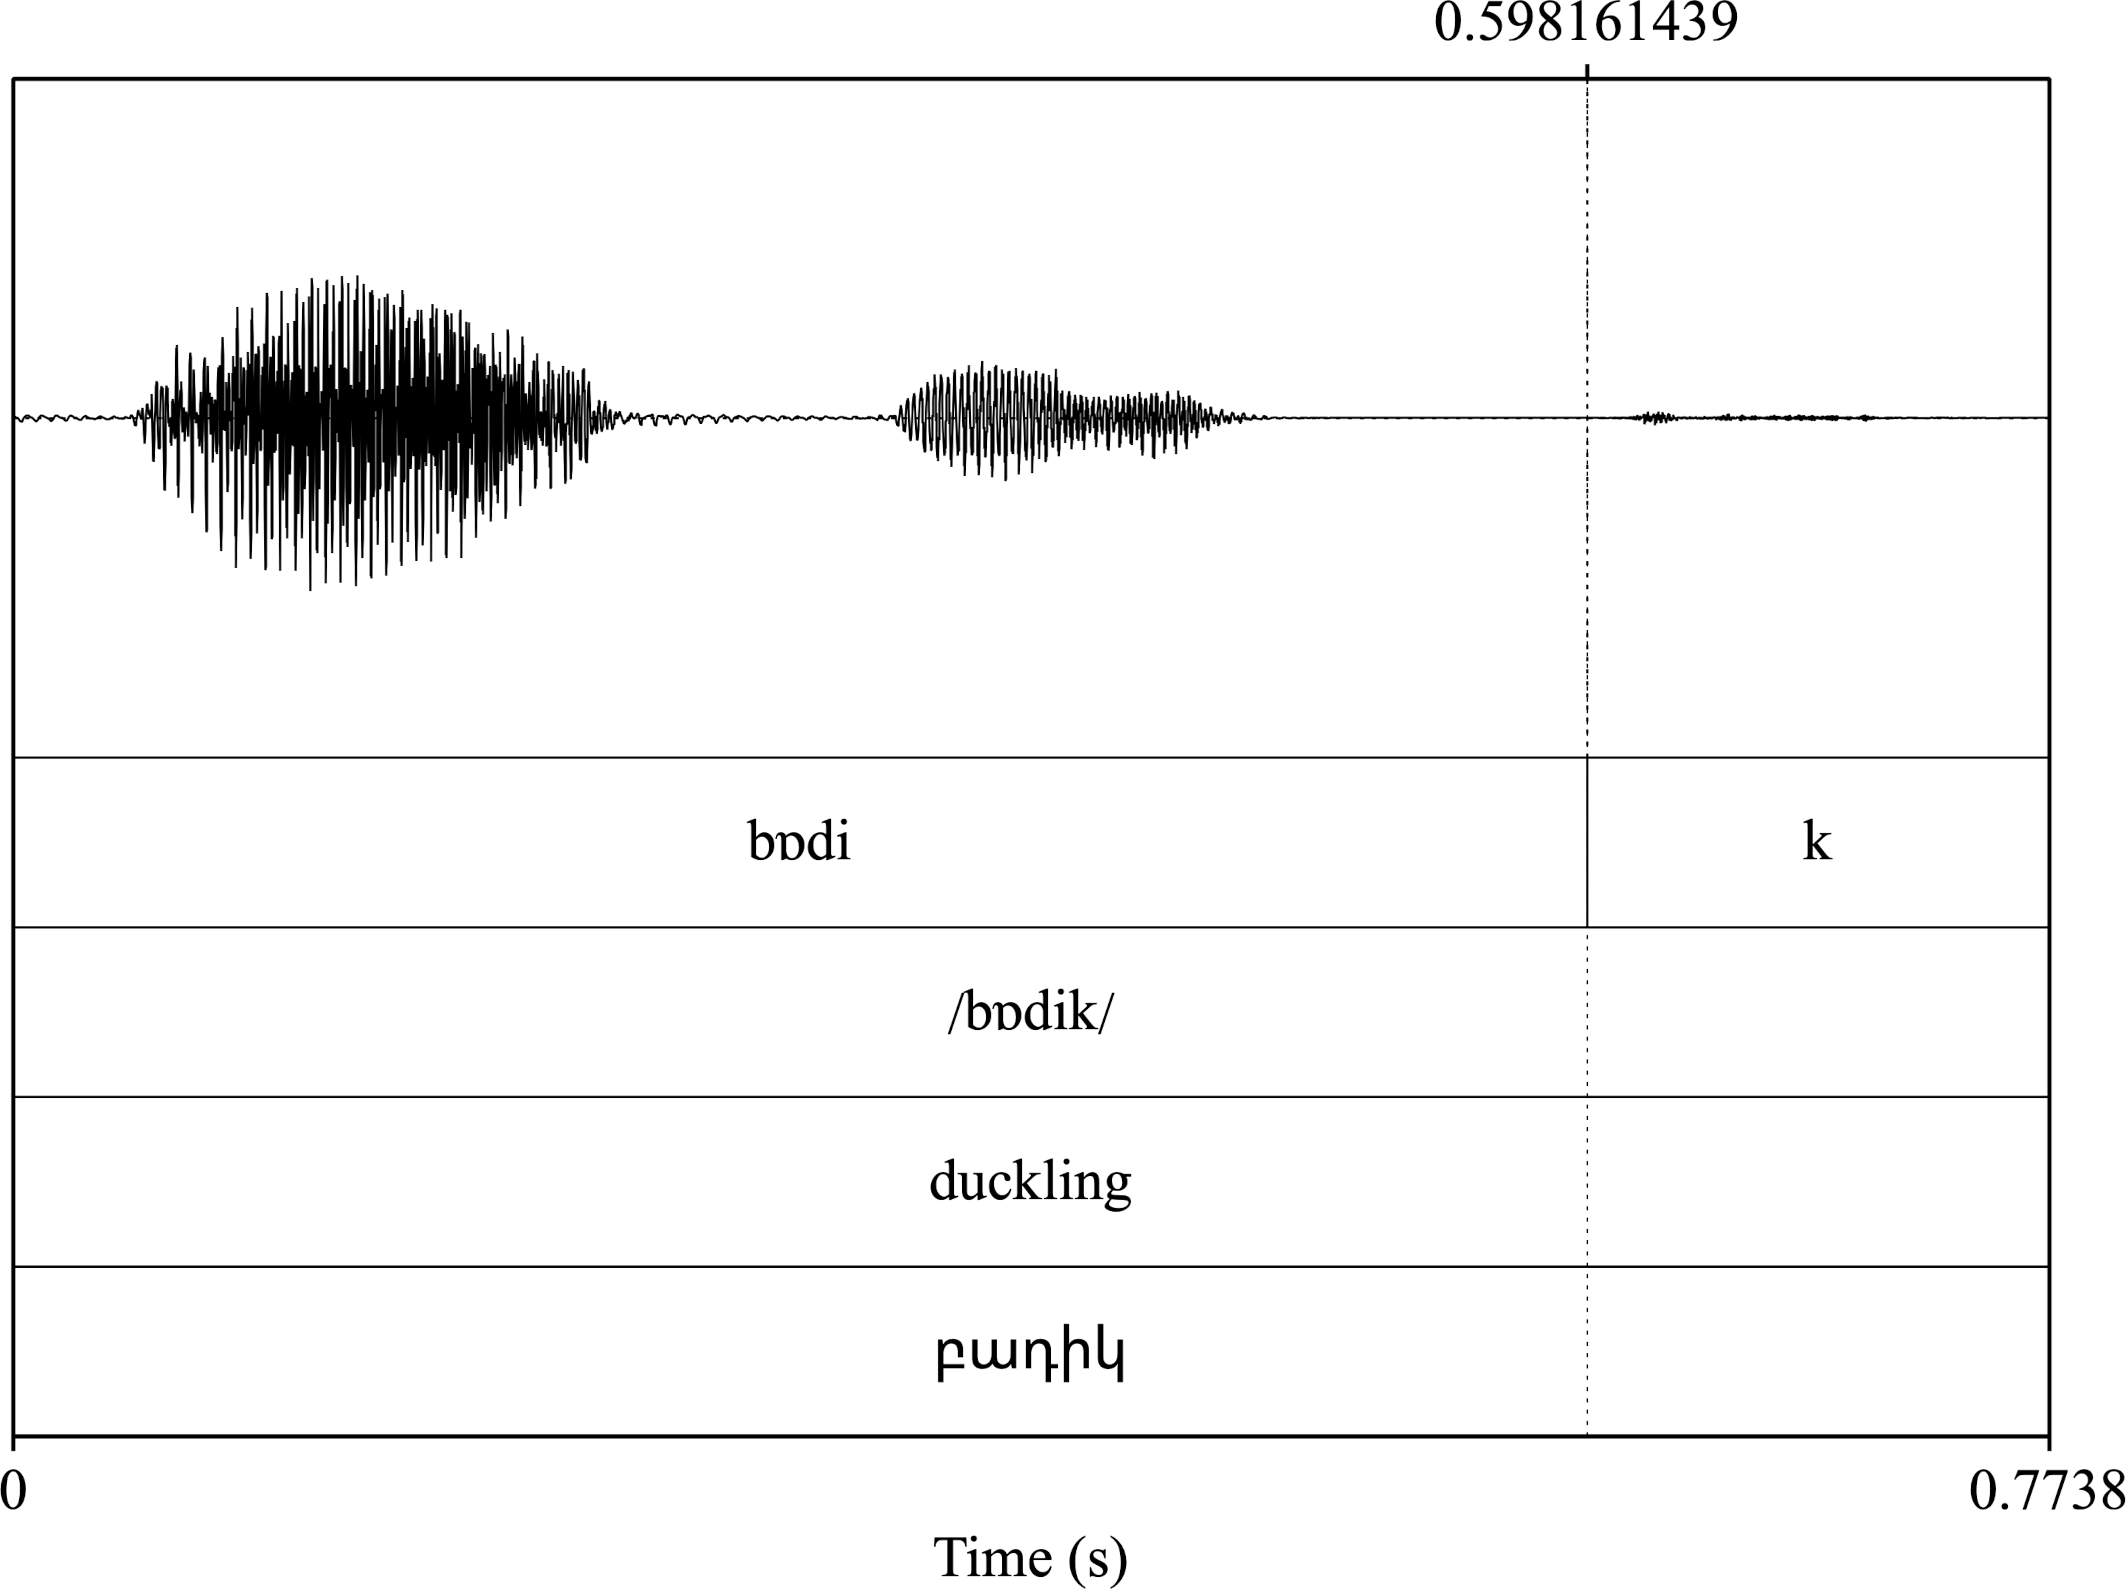
\includegraphics[width=\linewidth]{images/NK_NotEjective.png}
		\caption{Un-ejectivized final stop}
	\end{subfigure}%
	\begin{subfigure}[b]{0.5\textwidth}
		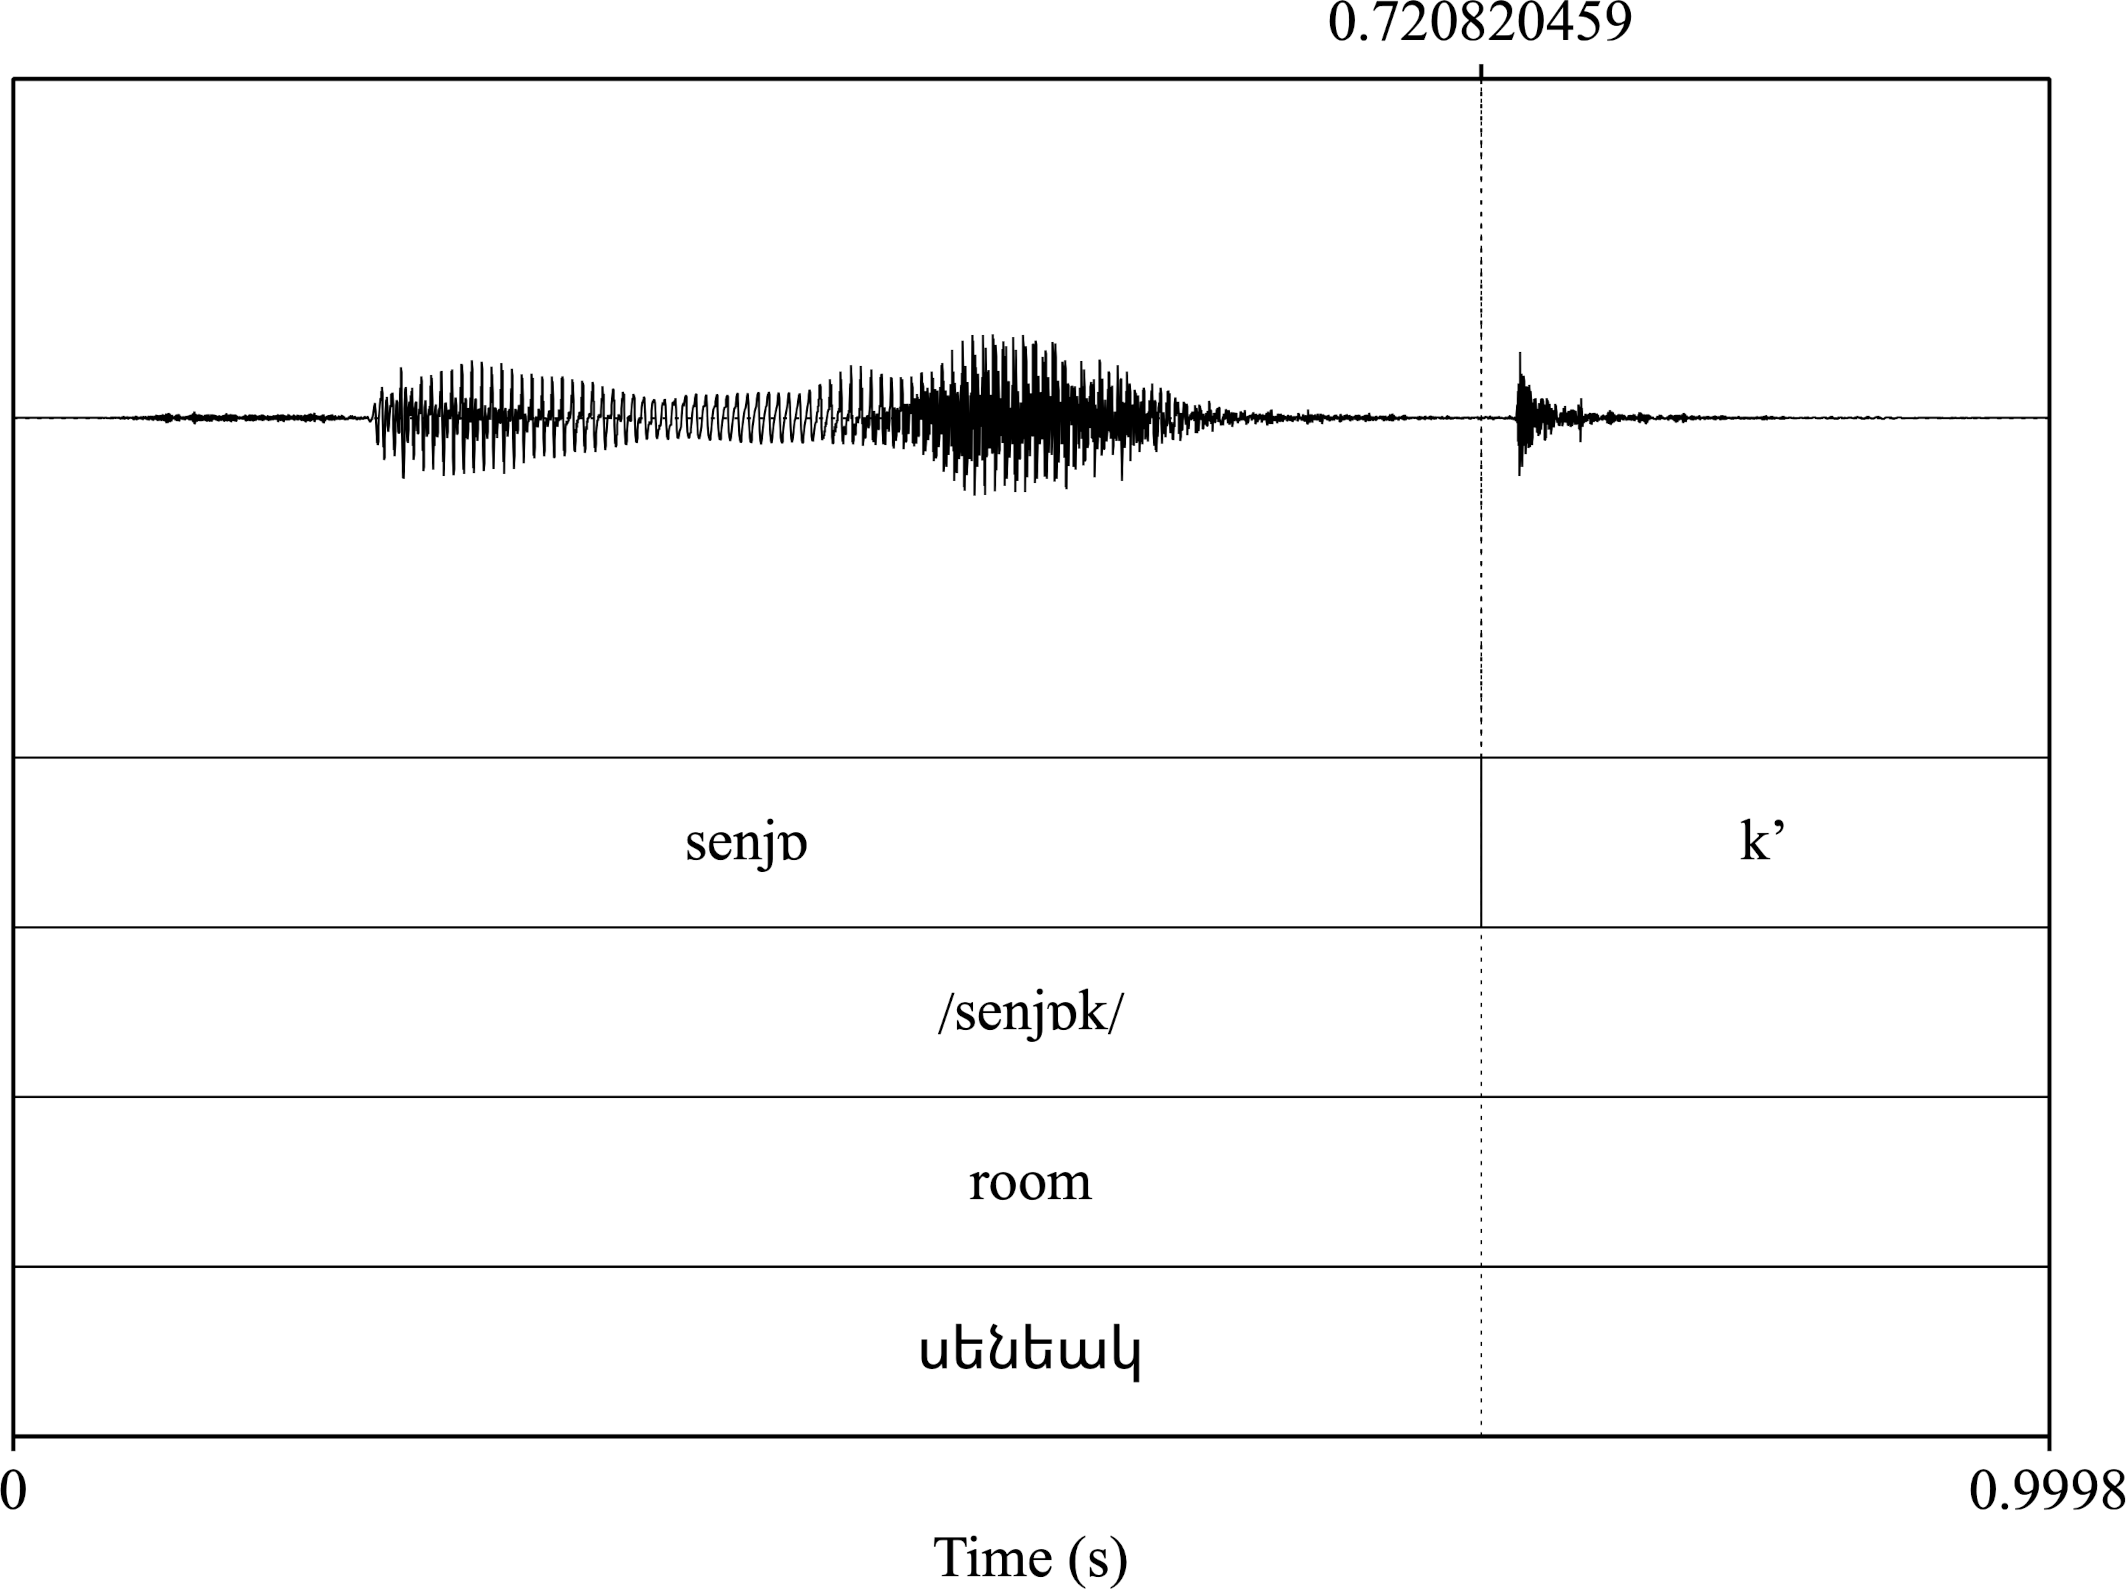
\includegraphics[width=\linewidth]{images/NK_Ejective.png}
		\caption{Ejectivized final stop}
	\end{subfigure}
\end{figure}


In general, for a given morpheme that is shared between   {\iaIA} and {\seaSEA}, the obstruents in that morpheme maintain the same laryngeal features in the two lects. That is, if a word begins   with a prevoiced stop in {\seaSE}, then it  also begins with a prevoiced stop in {\iaIA}. This correspondence is the general case. But we have encountered some morphemes where the {\iaIA} pronunciation utilizes a different laryngeal quality (Table \ref{tab:Phoon:Aspiration}). For example, the resultative participle suffix \armenian{-ած} is pronounced /{-ɑt͡s}/ in {\seaSE}, but is often pronounced as /{-ɒt͡sʰ}/ in {\iaIA} with aspiration in some speakers. NK always uses aspiration for this morpheme, while KM reports that she rarely does so. 

\begin{table}
	\caption{Unexpected aspiration in {\iaIA} from NK} \label{tab:Phoon:Aspiration}
	\fittable{\begin{tabular}{l lll l}
		\lsptoprule
		&{\seaAbbre} & {\iaAbbre} & \\\midrule
		\armenian{երգած}& {jeɾˈkʰ-ɑt͡s} & {jeɻˈkʰ-ɒt͡sʰ} &sing-{\rptcp} &  `sung'\\
		\armenian{կարդացած}& {kɑɾtʰ-ɑ-ˈt͡sʰ-ɑt͡s} & {kɒɻtʰ-ɒˈ-t͡sʰ-ɒt͡sʰ} & read-{\thgloss}-{\aor}-{\rptcp} & `read' \\
		\lspbottomrule
		\end{tabular}}
\end{table}

From AS's personal experience, the unexpected use of aspiration for the   affricate \armenian{{ծ}} /{t͡s}/ varies by speaker (Table \ref{tab:Phoon:AspirationVariable}). We speculate that this variable aspiration may be connected to variable ejectivization or glottalization of voiceless unaspirates. Variable ejectivization is reported for {\seaSE} \citep{Schirru-2012-LaryngealFeatureArmenianDialect,Seyfarth-2018-PlosiveVoicingAcousticsArmenian,ToparlakDolatian-2023-AerodynamicsarticulationwordfinalejectivesEasternArmenian}. AS likewise finds variable ejectivization for /{t͡s}/.
We speculate that what we report as aspiration might instead be a reflex of ejectivization. More data is of course needed.


\begin{table}
	\caption{Unexpected but variable aspiration of affricate /t͡s/ in {\iaIA} from NK\label{tab:Phoon:AspirationVariable}}
	\begin{tabular}{lll l}
		\lsptoprule
		&{\seaAbbre} & {\iaAbbre} & \\\midrule
		\armenian{ծնուել}& {t͡sənˈvel} & {t͡sənˈvel}$\sim${t͡sʰənvel} & `to be born'\\
		\armenian{գործածել}& {ɡoɾt͡sɑˈt͡sel} & {ɡoɻt͡sɒˈt͡sel}$\sim${ɡoɻt͡sʰɒˈt͡sʰel} & `to use' 
		\\ \lsptoprule
	\end{tabular}
\end{table}


In NK's speech (and in her family's), there were some words where the voiced stops were (variably) devoiced in her speech, and some where voiceless stops were (variably) voiced (Table \ref{tab:Phoon:AspirationVariable}). KM felt that such variable  voicing was more characteristic of heritage speakers in the diaspora than of speakers in Tehran. Note that these are all high-frequency words. 

\vfill
\begin{table}[H]
	\caption{High-frequency words with variable (de)voicing from NK and her family}\label{tab:Phono:Devoicing}
	\begin{tabular}{llll}
		\lsptoprule
		&{\seaAbbre}& {\iaAbbre} &  \\\midrule
		`(If) I come' & \textbf{ɡ}ɑm &\textbf{ɡ}ɒm, \textbf{k}ɒm  & \armenian{գամ}\\
		`door' & \textbf{d}ur &\textbf{d}ur, \textbf{t}ur  & \armenian{դուռ}\\
		`to put' & \textbf{d}ənel &\textbf{d}ənel, \textbf{t}ənel  & \armenian{դնել}\\
		`dance' & \textbf{p}ɑɾ &\textbf{p}ɒɻ, \textbf{b}ɑɻ  & \armenian{պար}\\
		`mouth' & \textbf{b}eɾɑn &\textbf{b}eɻɒn, \textbf{p}eɻɒn  & \armenian{բերան}\\
		`to bring' & \textbf{b}eɾel &\textbf{b}eɻel, \textbf{p}eɻel  & \armenian{բերել}\\
		`knife' & dɑnɑ\textbf{k} &dɒnɒ\textbf{k}, dɒnɒ\textbf{ɡ}  & \armenian{դանակ}\\
		`yesterday' & jeɾe\textbf{k} & eɻe\textbf{k}, eɻe\textbf{ɡ}  & \armenian{երեկ, էրեկ}\\
		`drawer' & dɑɾɑ\textbf{k} &dæɻæ\textbf{k}, dæɻæ\textbf{ɡ}  & \armenian{դարակ}\\
		\lspbottomrule
	\end{tabular}
	\label{tab:variabledevoicing}
\end{table}
\vfill\pagebreak

For such voicing differences, BV reports that using devoiced tokens like [tənel] instead of [dənel] `to put'   is the expected outcome in non-standard dialects of Iran, such as Urmia, Khoy, and Salmast \citep[34–40]{Asatryan-1962-KhoyUrmiaDialect},  Maragha \citep[83--89]{Adjarian-1926-MaraghaDialect}   and Keyvan (\armenian{Քեյվան}) \citep[187]{Baghramyan-1985-intermediatesubdialectGharadagh}. For   Tehrani {\iaIA}, such variation in devoicing may indicate the residue of dialect shifting, or possibly   a diglossic continuum between {\iaIA} and {\seaSEA}. 


\subsection{Rhotics}\label{section:phono:segmental:rhotic}
A stark difference between the two lects concerns their rhotics. {\seaSEA}   has a phonemic contrast between a flap /{ɾ}/ and a trill /{r}/. The flap is more frequent than the trill. Orthographically, the flap is represented by the grapheme \armenian{ր}, and the trill by \armenian{ռ}. Although {\iaIA}  also has a two-way rhotic distinction, the {\seaSE} flap corresponds to an {\iaIA} retroflex approximant /{ɻ}/. We contrast the two lects in Table \ref{tab:rhotic}.\footnote{The /{f}/ in `Raffi' is  variably geminated. The  /b/ in {\iaIA} `thin' is variably devoiced for NK.}


\begin{table}[p]
	\caption{Rhotic contrasts in {\seaSE} and {\iaIA}\label{tab:rhotic}}
	\resizebox{\textwidth}{!}{%
		\begin{tabular}{lllllll  }
			\lsptoprule
			&{\seaAbbre}&{\iaAbbre}&&{\seaAbbre}&{\iaAbbre}&\\
			&/{ɾ}/ &/{ɻ}/  &\armenian{ր}&/{r}/ &/{r}/ &\armenian{ռ}\\\midrule
			Initial &   {\textbf{ɾ}ɑˈfi} & {\textbf{ɻ}ɒˈfi}  & `Raffi (a name)'
			& {\textbf{r}eˈzin} & {\textbf{r}eˈzin} & `eraser' 
			\\
			&  & 				 &\armenian{Րաֆֆի}   & & &\armenian{ռեզին} 
			\\
			&&&
			& {\textbf{r}ɑzˈmik} &{\textbf{r}ɒzˈmik} & `Razmik (a name)' 
			
			\\
			&				&&&&  &\armenian{Ռազմիկ}
			\\
			Medial   & {bɑˈ\textbf{ɾ}ɑk} & {bɒˈ\textbf{ɻ}ɒk} & `thin' &   {ˈsɑ\textbf{r}ə} & {ˈsɒ\textbf{r}ə} & `cold' 
			\\
			&  &&\armenian{բարակ} &   & &\armenian{սառը}
			
			\\
			&
			{pɑˈ\textbf{ɾ}ɑp} &{pɒˈ\textbf{ɻ}ɒp} &  `available, empty'&
			{heˈ\textbf{r}u} & {heˈ\textbf{r}u} & `far'
			\\
			& && \armenian{պարապ}& 	& & 	\armenian{հեռու} 
			\\
			Final  & {ˈsɑ\textbf{ɾ}} &{ˈsɒ\textbf{ɻ}}  & `mountain' & {ˈbɑ\textbf{r}} & {ˈbɒ\textbf{r}} &`word'
			\\
			&  &	 &\armenian{սար} & & &\armenian{բառ}   
			\\
			& {ˈkɑ\textbf{ɾ}} &{ˈkɒ\textbf{ɻ}}  & `string'  &{ˈtɑ\textbf{r}}
			& {ˈtɒ\textbf{r}} & `letter'
			\\
			& &	&\armenian{կար} & & &  \armenian{տառ}  
			
			\\ \lspbottomrule\end{tabular}}
\end{table}


In general, if a word has a rhotic trill in {\seaSEA}, then it    has a trill in {\iaIA} as well. However, there were some high-frequency words where NK and other speakers preferred using a trill /r/ where {\seaSE} would use a flap /ɾ/ (Table \ref{tab:Phoon:RhoticTrillingVariable}). 

\begin{table}[p]
	\caption{High-frequency words that use a trill instead of an approximant}\label{tab:Phoon:RhoticTrillingVariable}
	\begin{tabular}{llll}
		\lsptoprule 
		&{\seaAbbre}& {\iaAbbre} &  \\\midrule
		`minute' & \textbf{ɾ}ope& \textbf{r}ope&  \armenian{րոպէ}  \\
		`war'& pɑte\textbf{ɾ}ɑzm & pɒte\textbf{r}ɒzm& \armenian{պատերազմ} \\  
		\lspbottomrule
	\end{tabular}
	\label{tab:trill not retro}
\end{table}

Some high-frequency words have a rhotic in {\seaSEA}, but the rhotic is optionally deleted in {\iaIA} (Table \ref{tab:Phoon:LossRhotic}).  The loss of the rhotic here may be related to the loss of rhotics in the perfective converb (\S\ref{section:morphophono:auxiliary}). 

\begin{table}[p]
	\caption{High-frequency words that lose a rhotic in {\iaIA}} \label{tab:Phoon:LossRhotic}
	\begin{tabular}{llll}
		\lsptoprule
		&{\seaAbbre}& {\iaAbbre} &  \\\midrule
		`to go' & je\textbf{ɾ}tʰɑl,   e\textbf{ɾ}tʰɑl, & e\textbf{ɻ}tʰɒl, etʰɒl  &  \armenian{երթալ, էրթալ, էթալ}  \\
		`when'& je\textbf{ɾ}pʰ & je\textbf{ɻ}pʰ, jepʰ& \armenian{երբ} \\  
		\lspbottomrule
	\end{tabular}
	\label{tab:tap lost}
\end{table}


The {\seaSE} flap  /ɾ/ is typically spirantized in some positions, such as word-finally (\cites[\S5]{Toparlak-2019-MAArmenianPhonetics}{Seyfarth-JIPAArmenian}). The {\iaIA} retroflex approximant  sounds similar to the American English alveolar approximant [ɹ] to our ears, but more retroflex like [ɻ].  A future acoustic or articulatory study can help in determining the exact place of articulation of this rhotic. 


Cross-linguistically, it is common to find that dialects differ in the phonetic realization of rhotics \citep{LadefogedMaddieson-1996-soundsWordldsLanguage,chabot-2019-WhatsWrongRhotic}.  It is rather rare to find languages with a phonemic retroflex approximant [ɻ] \citep[28]{Arsenault-2017-RetroflexionSouthAsiaTypologicalGeneticArealPatterns}. For example,  the UCLA Phonological Segment Inventory Database (UPSID) lists only 17 out of 451 languages (3.77\%) that have the phoneme /ɻ/  \citep{MaddiesonPrecoda-1989-UpdatingUPSID}.\footnote{\url{http://menzerath.phonetik.uni-frankfurt.de/S/S0763.html}} Most of these languages are in Australia. Similar results are obtained from the PHOIBLE 2.0 database at  306 out of 3020 languages (10\%) \citep{phoible}.  For the alveolar approximant [ɹ], this segment is acoustically quite similar to [ɻ]. This sound is cross-linguistically rare as well at 60 languages (2\%) in the PHOIBLE database. This segment is found particularly in Southeast Asia and in English. 



The origins of the {\iaIA} approximant could be due to language contact with Persian. Persian has a rhotic /{r}/ whose realization varies between a trill, tap, fricative, and approximant \citep{majidi-1991-persianFarsiJIPA,rafat-2010-socioPhoneticInvestigtionRhoticPersian}.  In a study on  Persian rhotics, \citet[675]{rafat-2010-socioPhoneticInvestigtionRhoticPersian} found that when  they were realized as   approximants, the approximants sounded retroflex.\footnote{However, the role of contact is likely limited. It is a stereotype that when {\iaAbbre} speakers speak Persian, they use the approximant /ɻ/ more often than Persian speakers. Classical Armenian may have had an approximant [ɹ] \citep[1040]{Macak-2017-PhonoClassicalArmenian}, so it's possible that {\iaAbbre} keeps [ɻ] as an archaism. But we suspect that it's more likely that the {\iaAbbre} /ɻ/ is an innovation.}

There is evidence that an approximant rhotic is  attested in   other Armenian dialects of Iran. In \citeauthor{Vaux-prep-NewJulfa}'s translation of  \citet{Adjarian-1940-NewJulfaDialect}'s grammar of New Julfa (Isfahan) Armenian, Vaux uses the IPA symbol [ɹ] to transcribe the letter \armenian{{ր}} (\S 6).  \citet[195]{allen-1950-notesPhoneticsEasternArmenianSpeaker} likewise reports a speaker of New Julfa who has a retroflex fricative that he transcribes as [ɹ].  It is an open question if the Tehrani [ɻ] and New Julfa [ɹ] are articulatorily different or the same.\footnote{The sound /ɹ/ is sometimes reported elsewhere in the Turkey-Caucasus-Iran region:  queer Turkish speakers from Istanbul \citep[11]{Kontovas-2012-LubuncaHistoricaldevelopmentIstanbulQueerSlang},  and the Muslim variety of the Hamshen dialect spoken in the village of Köprücü (Hopa province, northeastern Turkey) \citep[258]{Vaux-2007-HomshetsmaBook}. The sound [ɻ] is also reported in  the Iranian language of Kumzari in Oman \citep[25]{Anonby-2015-GrammarKumzariMixedPersoArabianLanguageOman}. For Turkish, it seems that approximants are generally attested    \citep{Nichols-2016-AcousticStudyTurkishRhotic},  possibly characteristic of ``white'' Turkish women and   also found in the northeastern parts of Turkey  (Nicholas Kontovas, p.c.). But it is unclear what is the exact place of articulation,  with some sources reporting an alveolar place while others report  a retroflex place \citep[12]{Tiras-2021-DissRhoticTurkish}. } 

Although the trill is phonemic in both lects, KM reports that the {\iaIA} trill feels ``not as trilled as in Eastern.'' This suggests that the trill uses a smaller number of tongue contacts in {\iaIA} than in {\seaSE}. Coincidentally, some dialects like {\swaSWA} have lost a phonemic trill for certain communities like in Lebanon \citep[16]{Vaux-1998-ArmenianPhono}.\footnote{In Armenian dialectology, Jahukyan \citep{Jahukyan-1972-ArmenianDiaolectology}     reports feature 23 as about ``confusion between /r/ and /ɾ/ in non-preconsonantal position''  in the dialects of Kuty, Hadjin, Tabriz, Tbilisi, Burdur, and Maragha.} Some communities in Canada still maintain   weak phonemic and weak articulatory distinctions between trills and flaps \citep{Tahtadjian-2020-WesterArmenianRhoticDifferentialPhoneticStudy}. KM's intuitions thus might indicate a slow language change toward  losing the trill.{\interfootnotelinepenalty=10000\footnote{%{\added}
	Don Stilo (p.c.) suggests that such a trajectory makes sense. Given that the   modern {\iaAbbre}  rhotic pair /ɻ, r/   likely descends from  a /ɾ, r/ pair (wih a flap), it is possible that the trill is slowly simplifying to become a flap.}}


\subsection{Other consonants}\label{section:phono:segmental:other cons}\largerpage
For completeness, we provide the rest of the consonantal inventory of {\iaIA} in Table \ref{tab:other consonants}. To our knowledge, the phonological properties of these remaining consonants do not differ between {\seaSE} and {\iaIA}.\footnote{%{\added}
	Don Stilo (p.c.) reports that the fricative /h/ of {\seaAbbre} and {\iaAbbre} sounds like a voiced form [ɦ]. We are not sure if this impression is accurate. Instrumental work on {\seaAbbre} reports that the fricative is generally a voiceless [h], but it has a voiced variant [ɦ] when intervocalic \citep[182--184]{Khachatryan-1988-ArmenianPhono}. In Armenian dialectology, early work by Adjarian (\citealt{Adjarian-1911-DialectologyBook}, translated in \citealt{Dolatian-prep-Adjarian}) reports a (possibly phonemic) [ɦ] in some dialects in Turkey (Erzurum/Karin, Mush, Van, Şebinkarahisar, Sebastia), but not in modern-day Armenia or Iran. Adjarian does however report in later work that the dialect of New Julfa in Iran possesses the phoneme /ɦ/   \citep[\S 5]{Adjarian-1940-NewJulfaDialect},   to which Jahukyan \citep[60]{Jahukyan-1972-ArmenianDiaolectology} adds Livasian (Chaharmahal). More recent sources also report /ɦ/ in many modern Armenian varieties spoken in the Republic of Armenia: Vardenis, Ashtarak, Koghb, Ghalacha/Berdavan, and Kamo/Gaver/New Bayazet \citep[58--59]{Jahukyan-1972-ArmenianDiaolectology}, and many more in the provinces of Gegharkunik  \citep{Katvlaryan-2018-ArmenianRepublicDialectChar1Geghargunik}  and Kotayk \citep{Katvalyan-2020-DialectBook}. 
}


\begin{table}[p]
	\caption{Other consonants in {\iaIA}}
	\label{tab:other consonants}
\small\tabcolsep=.66\tabcolsep\resizebox{\textwidth}{!}{%
		\begin{tabular}{ll ll ll ll}
			\lsptoprule 
			& &\multicolumn{2}{c}{Initial}&\multicolumn{2}{c}{Medial}&\multicolumn{2}{c}{Final}\\
			\cmidrule(lr){3-4}\cmidrule(lr){5-6}\cmidrule(lr){7-8}
			\armenian{մ} &
			/{m}/ 
			&  {ˈ\textbf{m}ɒɻtʰ} &  `man'
			
			&  {mɒˈ\textbf{m}-it͡sʰ} & `mom-{\abl}'
			
			&{dəˈɻɒ\textbf{m}} &  `Arm. dram'
			
			
			\\
			&
			&   &\armenian{մարդ}
			
			&    & \armenian{մամից}
			
			&  &  \armenian{դրամ}
			
			
			\\
			\armenian{ն} &
			/{n}/ 
			& {ˈ\textbf{n}ɒv}  &`ship'
			& {kʰəˈ\textbf{n}el}  &`to sleep'
			& {mɒˈt͡su\textbf{n}}  & `yogurt'
			\\
			&
			&    &   \armenian{նաւ}
			&    &  \armenian{քնել}
			&    & \armenian{մածուն}
			\\	\midrule 
			\armenian{ֆ} &
			/{f}/ 
			& {\textbf{f}ɒtʰiˈmɒ} &`Fatima'
			& {ɻɒˈ\textbf{f}i} &  `Raffi (name)'
			&{ˈkʰe\textbf{f}}&`party, mood'
			\\
			&
			
			&  &   \armenian{Ֆաթիմա}
			&  & \armenian{Րաֆֆի}
			&&\armenian{քէֆ}
			\\
			\armenian{ւ, վ} &
			/{v}/
			& {\textbf{v}oɾˈteʁ} &  `where'
			& {təˈ\textbf{v}oʁ} &   `giver'
			& {veˈɻe\textbf{v}} & `up'  
			\\
			&
			&   & \armenian{որտեղ}
			&  &\armenian{տուող}
			&   &\armenian{վերեւ}
			\\
			\armenian{ս} &
			/{s}/ 
			& {\textbf{s}iˈɻel} & `to love'
			& {ɒˈ\textbf{s}el} &  `to say'
			& {pɒˈkɒ\textbf{s}} & `missing'
			\\
			&
			
			&  & \armenian{սիրել}
			&   &\armenian{ասել}
			&   &\armenian{պակաս}
			\\
			\armenian{զ} &
			/{z}/
			& {ˈ\textbf{z}ɒŋɡ} &  `bell'
			& {ɒ\textbf{z}ɒˈtel} & `to free'
			& {ˈkʰe\textbf{z}} &  `you.{\dat}.{\sg}'
			\\
			&
			
			&  &\armenian{զանգ}
			& &\armenian{ազատել}
			&  &\armenian{քեզ}
			\\
			\armenian{շ} &
			/{ʃ}/ 
			& {ˈ\textbf{ʃ}eŋkʰ} & `building'
			&{pʰoˈ\textbf{ʃ}i}&  `dust'
			& {ˈt͡ʃɒ\textbf{ʃ}} &`food' 
			
			\\
			&
			
			&  &\armenian{շէնք}
			& &\armenian{փոշի}
			&   & \armenian{ճաշ}
			
			\\
			\armenian{ժ} &
			/{ʒ}/  
			& {\textbf{ʒ}əpˈtɒl} &  `to smile'
			&{uˈ\textbf{ʒ}eʁ}  &  `strong'
			& {ˈu\textbf{ʒ}}&`strength' 
			
			\\
			&
			
			& &\armenian{ժպտալ}
			& & \armenian{ուժեղ}
			& &\armenian{ուժ}
			
			\\
			\armenian{խ} &
			/{χ}/ 
			& {ˈ\textbf{χ}ɒt͡ʃʰ} &   `cross'
			& {t͡sɒˈ\textbf{χ}el} &  `to sell'
			& {ˈme\textbf{χ}} & `nail'
			\\
			&
			
			& &\armenian{խաչ}
			&  & \armenian{ծախել}
			&  & \armenian{մեխ}
			\\
			\armenian{ղ} &
			/{ʁ}/ 
			&{\textbf{ʁ}ɒzɒˈɻos}& `Lazarus'
			& {u\textbf{ʁ}ɒɻˈkel} &   `to send'
			& {ˈpʰo\textbf{ʁ}} &   `money'
			\\
			&
			
			& &\armenian{Ղազարոս}
			&  &\armenian{ուղարկել}
			&  &\armenian{փող}
			\\
			\armenian{յ, հ} &
			/{h}/ 
			& {ˈ\textbf{h}ɒt͡sʰ} &  `bread'
			& {mɒ\textbf{h}ɒˈnɒl} &  `to die'
			& {ˈʃɒ\textbf{h}} & `gain'
			
			\\
			&
			
			&  & \armenian{հաց}
			&  &\armenian{մահանալ}
			&  & \armenian{շահ}
			
			\\
			\midrule 
			\armenian{լ} &
			/{l}/ &{ˈ\textbf{l}ɒv} & `good'
			&{mo\textbf{l}oɻˈvel}  &  `to go astray'
			&  {ˈɡɒ\textbf{l}}&  `to come' 
			\\
			&
			& & \armenian{լաւ}
			&   & \armenian{մոլորուել}
			&  & \armenian{գալ}
			\\
			\armenian{յ} &
			/{j}/ 
			& {ˈ\textbf{j}eɻkʰ} & `song'
			& {tɒˈ\textbf{j}im} & `I give ({\subj}.{\pst})'
			&{ˈtʰe\textbf{j}}& `tea'
			\\
			&
			
			& &\armenian{երգ}
			&  & \armenian{տայիմ}
			& &\armenian{թէյ}
			\\
			\lspbottomrule 
		\end{tabular}}
\end{table}

The nasal /n/ becomes [ŋ] before velar stops /k, kʰ, ɡ/ (Table \ref{tab:Phono:nasalAssimilation}).

\begin{table}
	\caption{Examples of nasal place assimilation}\label{tab:Phono:nasalAssimilation}
	\begin{tabular}{lllll}
		\lsptoprule
		/zɒnɡ/ & $\rightarrow$ & ˈzɒŋɡ & `bell' & \armenian{զանգ}\\
		/menkʰ/ & $\rightarrow$ & ˈmeŋkʰ & `we' & \armenian{մենք}\\
		/tsʰɒnkɒnɒl/ & $\rightarrow$ & tsʰɒŋkɒˈnɒl & `to wish' & \armenian{ցանկանալ}\\
		\lspbottomrule
	\end{tabular}
\end{table}

In addition to the above consonantal phonemes, {\iaIA} has a surface glide [{w}] that is used to repair vowel hiatus (\ref{sent:Phono:Winsert}). This glide is discussed in \S\ref{section:morphophono:morphophono:vowel hiatus}. It is not a contrastive or phonemic segment.

\begin{exe}
	\ex \gll /kɒˈtu =e-m/ $\rightarrow $ [{kɒ.ˈtu.wem}]
	\\
	cat ={\auxgloss}-1{\sg}
	\\
	\trans	`I am a cat.'\label{sent:Phono:Winsert}
	\\
	\armenian{Կատու եմ։}
	
\end{exe}	

\subsection{Vowel inventory}\label{section:phono:segmental:vowel}
The vowel inventory is largely the same in both lects. We provide the basic vowel inventory in the two lects in Table \ref{tab:vowel inventory}. Most occurrences of the schwa are unwritten  in the orthography for {\seaSEA}. 


\begin{table}
	\caption{Vowel inventory across the lects\label{tab:vowel inventory}}
	\begin{tabular}{lllllll}
		\lsptoprule     Grapheme&\multicolumn{2}{c}{Phoneme} &\multicolumn{4}{l}{Example} \\
		&{\seaAbbre} &{\iaAbbre}& {\seaAbbre} &{\iaAbbre} &&\\\midrule
		\armenian{ա}		&/{ɑ}/&/{ɒ}/		&{t\textbf{ɑ}ˈɾi} &{t\textbf{ɒ}ˈɻi} &`year'&		\armenian{տարի}		\\
		\armenian{է, ե}	&/{e}/&/{e}/	&{t͡sʰoˈɾ\textbf{e}n} &{t͡sʰoˈɻ\textbf{e}n} &`wheat'&\armenian{ցորեն}		\\
		\armenian{ի}&/{i}/&/{i}/&{ˈkʰ\textbf{i}tʰ} &{ˈkʰ\textbf{i}tʰ}  &`nose'&	\armenian{քիթ}	\\
		\armenian{օ, ո}	&/{o}/&/{o}/ &{ˈv\textbf{o}ɾ} &{ˈv\textbf{o}ɻ} &`that'&\armenian{որ}\\
		\armenian{ու} &/{u}/&/{u}/		&{ˈd\textbf{u}r} &{ˈd\textbf{u}r} &`door'&\armenian{դուռ}\\
		\armenian{ը} &/{ə}/&/{ə}/ & {ˈmɑɾtʰ\textbf{ə}} &{ˈmɒɻtʰ\textbf{ə}} &`the man' & \armenian{մարդը}\\
		& & & {ɡ\textbf{ə}ˈɾel} &{ɡ\textbf{ə}ˈɻel} &`to write'& \armenian{գրել}\\ 
		\lspbottomrule
	\end{tabular}
\end{table}

Between the two lects, the main difference is that the low back vowel   is unrounded /{ɑ}/ in {\seaSE} but rounded /{ɒ}/ in {\iaIA}. The rounding of the low vowel is likely due to contact between {\iaIA} and Persian. Persian has a phonemic low back rounded  vowel /{ɒ}/ \citep{majidi-1991-persianFarsiJIPA}.\footnote{Anecdotally, BV has sometimes heard a rounded /ɒ/ in spoken {\seaEA} in Yerevan. In modern Persian, the low back rounded vowel /ɒ/ is acoustically unstable and can approach /{ɔ}/ \citep{esfandiari-2015-vowelClassificationVowelSpacePersian,mokari-2017-acousticDescriptionFarsiVowelsNativeSpeakerTehrani,aronowMchughMolnar-2017-pilotAcousticStudyModernPersianVowelsColloquialSpeec,jones-2019-corpusPhoneticStudyContemporaryPersianVowelCausalSpeech}. In our impressions, the {\iaIA} low vowel is much lower than the Armenian /{o}/. Although more acoustic data is needed, we speculate that the {\iaIA} /{ɒ}/ is truly [{ɒ}] and not [{ɔ}]. \label{footnote persian a}} 

When the low vowel /{ɒ}/ is next to a glide     /{j}/, the low vowel is still rounded (Table \ref{tab:Phono:LowBack}), but we suspect that it is not as rounded as in other contexts. More data is needed with finer acoustic measurements and across multiple speakers.\footnote{For the word `voice', the {\iaIA} word is [d͡zen] \armenian{ձեն} while the {\seaSE} word is the cognate [d͡zɑjn] \armenian{ձայն}. NK reports that {\iaIA}s sometimes say the word [d͡zɑjn] as a type of {\seaSE} borrowing, sometimes nativized as [d͡zɒjn].}

\begin{table}
	\caption{The low  back vowel stays rounded next to glide /{j}/}\label{tab:Phono:LowBack}
	\begin{tabular}{lll}
		\lsptoprule
		{}[{ˈhɒj}]  & `Armenian person' &\armenian{հայ}\\
		{}[mɒɻˈjɒm] & `Mariam' & \armenian{Մարիամ}\\
		\lspbottomrule
	\end{tabular}	
\end{table} 

\begin{sloppypar}
{\iaIA} likewise utilizes a   low front vowel /{æ}/ as a marginal phoneme (Table \ref{tab:low front vowel}). This vowel  appears in Persian loanwords. Some of these loanwords likewise exist in {\seaSE} (sometimes via a different route, such as from Turkish). But in {\seaSE}, the loanwords are nativized with the low back vowel /{ɑ}/. In general,  the front vowel does not appear in native Armenian words, but  we did find a  few  native constructions that contain it.\footnote{The word `drawer' is [{{dɑɾɑk}}] in {\seaSE}. In {\iaIA}, bi-dialectal KM pronounces the final stop as [k], while mono-lectal NK uses [ɡ]. We suspect this is just individual-level variation within the diaspora.}
\end{sloppypar}

\begin{table} 
	\caption{Low front vowel /{æ}/ in {\iaIA}}
	\label{tab:low front vowel}
	\resizebox{\textwidth}{!}{%
		\begin{tabular}{ll lll}
			\lsptoprule
			{\iaAbbre}&&&&cf. {\seaAbbre}\\\midrule
			{æˈɻæb} &`Arab' & \armenian{արաբ}&  from Persian&{ɑˈɾɑb}\\
			{mænˈʁæl} &`grill' &\armenian{մանղալ}&  from Persian  &{mɑnˈʁɑl} \\
			{læmæˈd͡ʒun} & `lahmacun' &\armenian{լահմաջուն} & from Turkish/Persian&{lɑhmɑˈd͡ʒun}\\
			{dæˈɻæɡ} & `drawer'&\armenian{դարակ}&   native &{dɑˈɾɑk}\\
			{mæˈhæt $\sim$ ˈmæt}& `a one'&\armenian{մի հատ}& native  & {mi ˈhɑt}\\ 
			\lspbottomrule
		\end{tabular}}
\end{table}

In the Armenian script, the front  vowel /æ/ is represented as  the symbol \armenian{ա} with umlaut       in dialectological  work. Because of variation across {\iaIA} speakers, we do not adopt this symbol in our orthographic forms, but instead use  a simple \armenian{ա}.

The use of /{æ}/ is     due to contact with Persian which has a phonemic /{æ}/ vowel \citep[286]{Mahootian-2002-PersianGrammar}. Although contemporary {\iaIA} has /{æ}/ as a marginal phoneme, it is possible that earlier stages of {\iaIA} did not. \citet[368]{zamir-1982-variationStandardPersianSociolinguisticStudy} reports that his sample of {\iaIA}s did not have the phoneme /{æ}/  when they spoke Persian. Their accent of Persian was characterized by replacing the Persian /{æ}/ with a back variant. Similarly for New Julfa Armenian in Isfahan,  Adjarian \citep[\S 7]{Adjarian-1940-NewJulfaDialect} reports that in  the 1910s/1920s, /æ/ was slowly getting introduced in the speech of young Armenians. See the translation by \citet{Vaux-prep-NewJulfa}. This suggests that the introduction of /æ/ as a marginal phoneme is both recent and widespread in the Armenian dialects of Iran.\footnote{\citet[183]{allen-1950-notesPhoneticsEasternArmenianSpeaker} reports a speaker from New Julfa who only has a low vowel  without any indication of rounding or fronting. This speaker does however self-report as being heavily influenced by Yerevan {\seaSEA}. }




As an interesting diachronic fact, there are some words that are pronounced with either   [uj]  or [ju] in {\seaSEA}, but which are pronounced with [u] in {\iaIA} (Table \ref{tab:uj ju}). But this is not a general rule   because there are some words that are pronounced with [uj] or [ju] in both varieties.\footnote{%{\added}
	For {\swaAbbre}, the {\seaAbbre} [ju] sequence corresponds to [ʏ]: [t͡sʏn] `snow'. Don Stilo reports that he may have heard some {\iaAbbre} speakers use a front vowel as well [d͡zʏn]. Unfortunately, we have not been able to replicate this form with our speaker pool.}

\begin{table}
	\caption{Dialectal variation in [uj] and [ju] sequences\label{tab:uj ju}}
	\begin{tabular}{ll lll }
		\lsptoprule
		& \multicolumn{2}{l}{Changing /uj/, /ju/ or [u]}& \multicolumn{2}{l}{Keeping /uj, ju/}\\
		\midrule
		& `sister'& `snow' & 	 `color'  & `other' 		\\
		{\seaAbbre}  & [kʰujɾ]  & [d͡zjun]& [ɡujn]& [mjus]		\\
		{\iaAbbre} &  [kʰuɻ] &  [d͡zun]& [ɡujn] & [mjus]	\\
		& \armenian{քոյր}& \armenian{ձիւն} & \armenian{գոյն} & \armenian{միւս}\\ \lspbottomrule
	\end{tabular}
\end{table}

\section{Suprasegmental phonology}\label{section:phono:suprasegmental}


In general, we did not find significant differences between {\seaSE} and {\iaIA}  in terms of syllable structure (\S\ref{section:phono:suprasegmental:syllable}). There are some differences in word stress (\S\ref{section:phono:suprasegmental:stress}). Intonational differences are   salient because {\iaIA} has borrowed aspects of Persian intonation (\S\ref{section:phono:suprasegmental:intonation}).

\subsection{Syllable structure }\label{section:phono:suprasegmental:syllable}

The syllable structure of {\iaIA}  is not substantially different from that of {\seaSE} (Table \ref{tab:syllable}). In {\iaIA}, the typical syllable is at most CVCC.  Complex onsets are limited to /Cj/ clusters, and intervocalic /Cj/ clusters are usually syllabified together into the same syllable. Complex codas generally have falling sonority. The segment /{kʰ}/ can follow any type of cluster. Phonologically, this segment is an extrasyllabic appendix. 

\begin{table}
	\caption{Syllable shapes in {\iaIA}\label{tab:syllable}}
	\begin{tabular}{l ll l}
		\lsptoprule  V& {ˈu} &`and' & \armenian{ու}   \\
		CV& {ˈdu} &`you ({\nom}.{\sg})ˈ & \armenian{դու}\\
		VC& {ˈɒpʰ} &`shore' & \armenian{ափ}\\
		CVC& {ˈpʰiʁ} &`elephant' & \armenian{փիղ}\\
		CVCC& {ˈmɒɻtʰ} &`man' & \armenian{մարդ}\\
		\midrule 
		CjVCC &{ˈkjɒŋkʰ} & `life' & \armenian{կեանք}
		\\
		CV.CjVC &{seˈnjɒk }& `room' & \armenian{սենեակ}
		\\
		CVCkʰ & {ˈpetkʰ}&`need'& \armenian{պէտք}
		\\
		CVCCkʰ & {ˈkuɻt͡skʰ}&`breast' & \armenian{կուրծք}
		\\ \lspbottomrule 
	\end{tabular}
\end{table}

All the above generalizations are likewise found in {\seaSEA}. For general overviews of syllable structure in {\seaSEA}, see \citet[\S1, 3]{Vaux-1998-ArmenianPhono}. For a discussion of the final appendix \textit{{-kʰ}} in {\seaSE}, see \citet[83]{Vaux-1998-ArmenianPhono},  \citet{VauxWolf-2009-Appendix}, and \citet[\S 5]{Dolatian-2020-NLLTArmenianReduction}.

An exception to the above generalizations concerns word-initial sibilant-stop sequences. Such clusters variably undergo schwa prothesis in both {\seaSE} and {\iaIA} (Table \ref{tab:Phono:Prothesis}). In modern Eastern, the norm is for schwa prothesis to not apply. In our elicitations from {\iaIA} speakers, most cases of sibilant-stop clusters did not undergo prothesis. When a schwa is absent, the sibilant is analyzed as an extrasyllabic appendix (\cites[83ff]{Vaux-1998-ArmenianPhono}{VauxWolf-2009-Appendix}{Dolatian-prep-Schwa}). 



\begin{table}
	\caption{Schwa prothesis in sibilant-stop clusters}\label{tab:Phono:Prothesis}
	\begin{tabular}{ ll l }
		\lsptoprule
		zɡujʃ & `caution'  & \armenian{զգոյշ}\\
		stɒnɒl & `to receive' 	& \armenian{ստանալ}\\
		(ə)skəsel & `to start'& \armenian{սկսել}\\
		əzɡɒl & `to feel'& \armenian{զգալ}\\
		skizb & `beginning'& \armenian{սկիզբ}\\
		\lspbottomrule
	\end{tabular}
\end{table}



\subsection{Lexical stress}\label{section:phono:suprasegmental:stress}
{\iaIA} seems to utilize the same lexical stress system as {\seaSEA}.  For an overview of lexical stress in {\seaSEA}, see \citet[\S4]{Vaux-1998-ArmenianPhono} and \citet{Dolatian-2020-NLLTArmenianReduction}. But there are differences in irregular stress.

\subsubsection{Regular  stress}\label{section:phono:suprasegmental:stress:reg}
Within the morphological word, stress is generally final on the rightmost non-schwa vowel (\ref{sent:Phono:regStress}). This means that regular stress is  on the final syllable if that syllable has a non-schwa nucleus.  Suffixation of non-schwa suffixes triggers stress shift.\footnote{Prescriptively, the suffix \armenian{-ութիւն} (\armenian{-ություն} in {\seaSE}) is pronounced as [{-utʰjun}]. But in casual speech, the stop-glide sequence  usually  undergoes affrication.  \label{footnote utjun}} 

\begin{exe}
	\ex \label{sent:Phono:regStress}
	\begin{xlist}
		\ex \makebox[3cm][l]{{t͡ʃɒˈ\textbf{kɒt}}}\makebox[3cm][l]{`forehead'}\armenian{ճակատ}
		
		\makebox[3cm][l]{{t͡ʃɒkɒt-ɒ-ˈ\textbf{ɡiɻ}}}\makebox[3cm][l]{`destiny'}\armenian{ճակատագիր}

  
		\ex \makebox[3cm][l]{{uˈ\textbf{ɻɒχ}}}\makebox[3cm][l]{`happy'}\armenian{ուրախ}
		
		\makebox[3cm][l]{{uɻɒχ-uˈ\textbf{t͡ʃʰun}}}\makebox[3cm][l]{`happiness'}\armenian{ուրախութիւն}
	\end{xlist}
\end{exe}

Note that [ɒ-{ɡiɻ}] is the compound linking vowel {\lvgloss} and the root [ɡiɻ] `writing'. The suffix [-ut͡ʃʰun] is a nominalizer suffix. 



If the final syllable has a schwa, then stress is on the penultimate syllable (\ref{sent:Phono:regStressSchwa}). 

\begin{exe}
	\ex  \label{sent:Phono:regStressSchwa}
	\begin{xlist}
		
		\ex \makebox[3cm][l]{{t͡ʃɒˈ\textbf{kɒ}t-ə}}\makebox[5cm][l]{`forehead-{\defgloss}'}\armenian{ճակատը}
		
		\makebox[3cm][l]{}`the forehead'
		
		\makebox[3cm][l]{{t͡ʃɒˈ\textbf{kɒ}t-əs}}\makebox[5cm][l]{`forehead-{\possFsg}'}\armenian{ճակատս}
		
		\makebox[3cm][l]{}`my forehead'
		
		\makebox[3cm][l]{{t͡ʃɒˈ\textbf{kɒ}t-ət}}\makebox[5cm][l]{`forehead-{\possSsg}'}\armenian{ճակատդ}
		
		\makebox[3cm][l]{}`your forehead'
		
	\end{xlist}
\end{exe}





Besides final schwas, stress is avoided on clitics (\ref{sent:Phono:regStressClitic}).  

\begin{exe}
	\ex \label{sent:Phono:regStressClitic}
	\begin{xlist}
		
		\ex \makebox[3cm][l]{{t͡ʃɒˈ\textbf{kɒ}t=el}}\makebox[5cm][l]{`forehead=also'}\armenian{ճակատ էլ}
		
		\makebox[3cm][l]{}`also forehead'
		
		\makebox[3cm][l]{{t͡ʃɒˈ\textbf{kɒ}t=ɒ}}\makebox[5cm][l]{`forehead={\auxgloss}'}\armenian{ճակատ ա}
		
		\makebox[3cm][l]{}`is forehead'
		\ex \makebox[3cm][l]{{uˈ\textbf{ɻɒ}χ=el}}\makebox[5cm][l]{`happy=also'}\armenian{ուրախ էլ}
		
		\makebox[3cm][l]{}`also happy'	
		
		\makebox[3cm][l]{{uˈ\textbf{ɻɒ}χ=ɒ}}\makebox[5cm][l]{`happy={\auxgloss}'}\armenian{ուրախ ա}
		
		\makebox[3cm][l]{}`is happy'
		
		
	\end{xlist}
\end{exe}

If the word takes a cluster of clitics, stress stays inside the word (\ref{sent:Phono:regStressCliticCluster}). 

\begin{exe}
	\ex \label{sent:Phono:regStressCliticCluster}\begin{xlist}
		\ex \makebox[3cm][l]{{t͡ʃɒˈ\textbf{kɒ}t=el=ɒ}}\makebox[5cm][l]{`forehead=also={\auxgloss}'}\armenian{ճակատ էլ	ա}
		
		\makebox[3cm][l]{}`is also a  forehead'
		\ex \makebox[3cm][l]{{uˈ\textbf{ɻɒ}χ=el=ɒ}}\makebox[5cm][l]{`happy=also={\auxgloss}'}\armenian{ուրախ էլ	ա}
		
		\makebox[3cm][l]{}`is also happy'
	\end{xlist}
\end{exe}


\subsubsection{Irregular  stress}\label{section:phono:suprasegmental:stress:irreg}
We catalog some morphological contexts which trigger exceptional non-final stress. 


A systematic exception to final stress involves the negation prefix /{t͡ʃʰ-}/ (pronounced [{t͡ʃʰə-}] before consonants), as in Table \ref{tab:Phono:IrregStress}. In both periphrastic and synthetic tenses, the negation prefix attracts primary stress. For periphrastic tenses, the prefix is added to the auxiliary, and the auxiliary takes stress. In synthetic tenses, the prefix is added directly to the verb. The first syllable of the verb takes stress, even if the first syllable has a schwa. 

\begin{table}
	\caption{Irregular stress in negation }\label{tab:Phono:IrregStress}
	
	\begin{tabular}{lll}
		\lsptoprule
		& Positive & Negative\\\midrule
		`I am singing' & jeɻˈ\textbf{kʰ-um} e-m & ˈ\textbf{t͡ʃʰ-e-m} jeɻkʰ-um    \\
		& sing-{\impfcvb} {\auxgloss}-1{\sg}&  {\neggloss}-{\auxgloss}-1{\sg} sing-{\impfcvb}\\
		& \armenian{երգում եմ}& \armenian{չեմ երգում}\\
		\addlinespace 					
		`he  took' & veɻ-t͡sˈ\textbf{ɻ-ɒ-v} &  ˈ\textbf{t͡ʃʰə}-veɻ-t͡sɻ-ɒ-v \\
		& take-{\caus}-{\pst}-3{\sg}&{\neggloss}-take-{\caus}-{\pst}-3{\sg}\\
		& \armenian{վերցրաւ}& \armenian{չվերցրաւ}\\
		\addlinespace 				
		`he  did' & ɒˈ\textbf{ɻ-ɒ-v} &  ˈ\textbf{t͡ʃʰ-ɒ}ɻ-ɒ-v  \\
		& do-{\pst}-3{\sg}&{\neggloss}-do-{\pst}-3{\sg}\\
		& \armenian{արաւ}& \armenian{չարաւ}\\
		\addlinespace 			
		`he  fell' & əŋˈ\textbf{ɡ-ɒ-v} &  ˈ\textbf{t͡ʃʰ-ə}ŋɡ-ɒ-v  \\
		& fall-{\pst}-3{\sg}&{\neggloss}-fall-{\pst}-3{\sg}\\
		& \armenian{ընկաւ}& \armenian{չընկաւ}\\
		\lspbottomrule
	\end{tabular}
\end{table}

Negation stress is reported in {\iaIA} dialogues from \citet{ShakibiBonyadi-1995-ShortSurveyArmenianLanguageTehrani}. In HD's experience, negation stress    is likewise attested in {\swaSWA} in both synthetic and periphrastic tenses. However in {\seaSEA}, negation attracts stress in only periphrastic tenses, not synthetic \citep[77]{Margaryan-1997-ArmenianPhonology}. The fact that {\iaIA} has negation-sensitive stress may be due to language contact with Persian, where negation is a stressed prefix \citep{Kahnemuyipour-2009-SyntaxSententialStress}. 





Another morphological exception for final stress comes from ordinals (\tabref{tab:ordStressIrregu}). The ordinal suffixes /-ɻoɻtʰ, -eɻoɻtʰ/ assign stress to the previous syllable \citep[cf.][132ff]{Vaux-1998-ArmenianPhono}. For more examples, see \S\ref{section:funct:num:ord}.  When an inflectional suffix or clitic is added after the ordinal suffix, irregular stress is lost and we get regular  stress on the rightmost non-schwa and non-clitic vowel.

\begin{table}
	\centering   \caption{Irregular stress in ordinals in Iranian Armenian}
	\label{tab:ordStressIrregu}
	\resizebox{\textwidth}{!}{%
		\begin{tabular}{lllll}
		\lsptoprule 
		a. Cardinal & 	`two'          & eɻˈ\textbf{ku}                 & 2           & \armenian{էրկու}            \\
		&		`five'       & ˈ\textbf{hiŋɡ}    & 5     & \armenian{հինգ}  \\
		\addlinespace 
		b. Ordinal & 		`second'   & ˈ\textbf{jek}-ɻoɻtʰ     & 2-{\ord}   & \armenian{երկրորդ}  \\
		&	`fifth'  & ˈ\textbf{hiŋɡ}-eɻoɻtʰ   & 5-{\ord}  & \armenian{հինգերորդ}
		\\
		\addlinespace 
		c. Adding /-i/& `to the second one'   & {jek}-{ɻoɻ}ˈ\textbf{tʰ-i-n}     & 2-{\ord}-{\dat}-{\defgloss}  & \armenian{երկրորդին}  \\
		&	`to the fifth one'   & {hiŋɡ}-e{ɻoɻ}ˈ\textbf{tʰ-i-n}     & 2-{\ord}-{\dat}-{\defgloss}  & \armenian{հինգերորդին}  \\
		\addlinespace 
		d. Adding /-ə/ & 	`the second one'   & {jek}-ˈ\textbf{ɻoɻ}tʰ-ə     & 2-{\ord}-{\defgloss}  & \armenian{երկրորդը}  \\
		& 	`the fifth one'   & {hiŋɡ}-eˈ\textbf{ɻoɻ}tʰ-ə     & 5-{\ord}-{\defgloss}  & \armenian{հինգերորդը}  \\
		\addlinespace 
		e.  Adding clitic & `he is second'   & {jek}-ˈ\textbf{ɻoɻ}tʰ  =ɒ    & 2-{\ord}={\auxgloss}  & \armenian{երկրորդ ա}  \\
		&	`he is fifth'   & {hiŋɡ}-eˈ\textbf{ɻoɻ}tʰ=ɒ     & 5-{\ord}={\auxgloss}  & \armenian{հինգերորդ ա}  \\
		\lspbottomrule 
	\end{tabular}}
\end{table}

Beyond this section, we generally avoid marking stress    in order to reduce clutter. Unless otherwise stated, stress is  on the rightmost non-schwa and non-clitic vowel. 

\subsection{Prosodic phonology and intonation}\label{section:phono:suprasegmental:intonation}

Above the word, there is relatively little known about the prosodic structure of phrases and clauses in any Armenian lect (\cites[27ff]{Fairbanks-1948-PhonologyMorphoWestern}[14ff]{Johnson-1954-EastArmGrammar}{Ghukasyan-1990-WesternEasternArmenianIntonation}{ToparlakDolatian-202x-IntonationFocusMarkingWesternArmenian}{Dolatian-2022-InterfaceNuclearStressWesternArmenianTurkishPersian}).  There is however one aspect of {\iaIA} prosodic phonology which stands out from {\seaSEA}. This concerns the intonational structure of questions.  We briefly overview the main properties of {\iaIA} interrogatives, using common notation from the autosegmental-metrical tradition on intonational phonology \citep{Pierrehumbert-1980-phonologyPhoneticsEnglishIntonation,Ladd-1986-IntonationalPhrasingRecursiveProsodic,jun-2007-prosodicTypologyPhonologyIntonationPhrasing}. The recordings from this subsection can be found in the online archive.\footnote{\url{https://github.com/jhdeov/iranian_armenian}}

In   a basic SOV sentence in the present tense (\ref{example: sov dec sentence}), verbal inflection is periphrastic. The verb is in the form of the imperfective converb, and tense-agreement marking is on an auxiliary.  If the object is morphologically bare, then it carries sentential stress (nuclear stress, underlined). The auxiliary is cliticized to the bare object.\footnote{The distribution of this auxiliary is complex in {\seaSE} and {\iaIA} (\S\ref{section:morphophono:auxiliary:syntax}). For further data and discussion, see \citet{Tamrazian-1994-ArmenianSyntax,Megerdoomian-2009-ThesisBook,KahnemuyipourMegerdoomian-2011-secondcliticvP,KahnemuyipourMegerdoomian-2017-positionalDistriutionFocus}.} Declarative sentences end in falling intonation.\largerpage[2]




\begin{exe}
	\ex 
	\begin{xlist}
		\ex \textit{Declarative    SOV sentence with an auxiliary}\label{example: sov dec sentence}
		
		{%\resizebox{.85\textwidth}{!}{%
				\begin{tabular}{llllll}
					i.& {mɑɾjɑ-n}& {\uline{ɡiɾkʰ}}&={e}& {kɑɾtʰ-um}$\searrow$&({\seaAbbre})
					\\
					&\multicolumn{5}{l}{\armenian{Մարիան գիրք է կարդում։}}
					\\
					
					ii. & {mɒɻjɒ-n}&   {\uline{ɡiɻkʰ}}&={ɒ}& {kɒɻtʰ-um}$\searrow$&({\iaAbbre})
					\\
					
					& Maria-{\defgloss}&book&={\auxgloss}& read-{\impfcvb} & 
					\\
					&\multicolumn{5}{l}{`Maria is  reading books.'
					}   
					\\ 
					&\multicolumn{5}{l}{\armenian{Մարիան գիրք ա կարդում։}}
					\\
				\end{tabular} 
			}

			\ex \textit{Polar question} \label{example: sov polar sentence}
			
			{%\resizebox{.85\textwidth}{!}{%
					\begin{tabular}{llllll}
						i.& {mɑɾjɑ-n}& {\uline{ɡiɾkʰ}}$\nearrow$&={e}& {kɑɾtʰ-um}$\searrow$&({\seaAbbre})
						\\
						&\multicolumn{5}{l}{\armenian{Մարիան գի՞րք է կարդում։}}
						\\
						ii. & {mɒɻjɒ-n}&   {\uline{ɡiɻkʰ}}$\nearrow$&={ɒ}& {kɒɻtʰ-um}$\nearrow$&({\iaAbbre})
						\\
						& Maria-{\defgloss}&book&={\auxgloss}& read-{\impfcvb} & 
						\\
						&\multicolumn{5}{l}{`Is Maria reading  books?'
						}
						\\
						&\multicolumn{5}{l}{\armenian{Մարիան գի՞րք ա կարդում։}}
						\\
						
					\end{tabular} 
				}			
			\end{xlist}
			
		\end{exe}
		
		To form polar questions, the only strategy in {\seaSE} and {\iaIA} is   intonational. In {\seaSEA}, there is a significant rise in pitch on the bare object in (\ref{example: sov polar sentence}-i). The sentence ends in falling intonation \citep[cf.][]{Ghukasyan-1990-WesternEasternArmenianIntonation,Ghukasyan-1999-EasternYesNoQuestionIntonation}. In contrast in {\iaIA}, there is both a rise on the object and a sentence-final rise (\ref{example: sov polar sentence}-ii). 
		
		For illustration, Figure \ref{fig:dec polar basic eastern iranian}  shows the pitch track of the declarative sentence (\ref{example: sov dec sentence}) and its corresponding polar question (\ref{example: sov polar sentence}) in both {\seaSE} and {\iaIA}.  	The {\iaIA} recordings are from NK. The {\seaSEA} recordings are from AT. We annotate the perceived nucleus with the H* symbol, sentence-final fall with L\%, and sentence-final rise with H\%.
		
 
		
		
		As is clear, both declarative sentences end in L\%. The {\iaIA} polar question has H\%. For {\seaSE}, both the declarative and polar question   end in a L\%. The main difference is the level of pitch on the nuclear stressed word [{ɡiɾkʰ}] `book'.
		
	\vfill
	\begin{figure}[H]
		\caption{Pitch track of declarative (\ref{example: sov dec sentence}) and polar question (\ref{example: sov polar sentence})   in   {\seaAbbre}   an {\iaAbbre} \label{fig:dec polar basic eastern iranian}}
		\begin{subfigure}[b]{0.5\textwidth}
			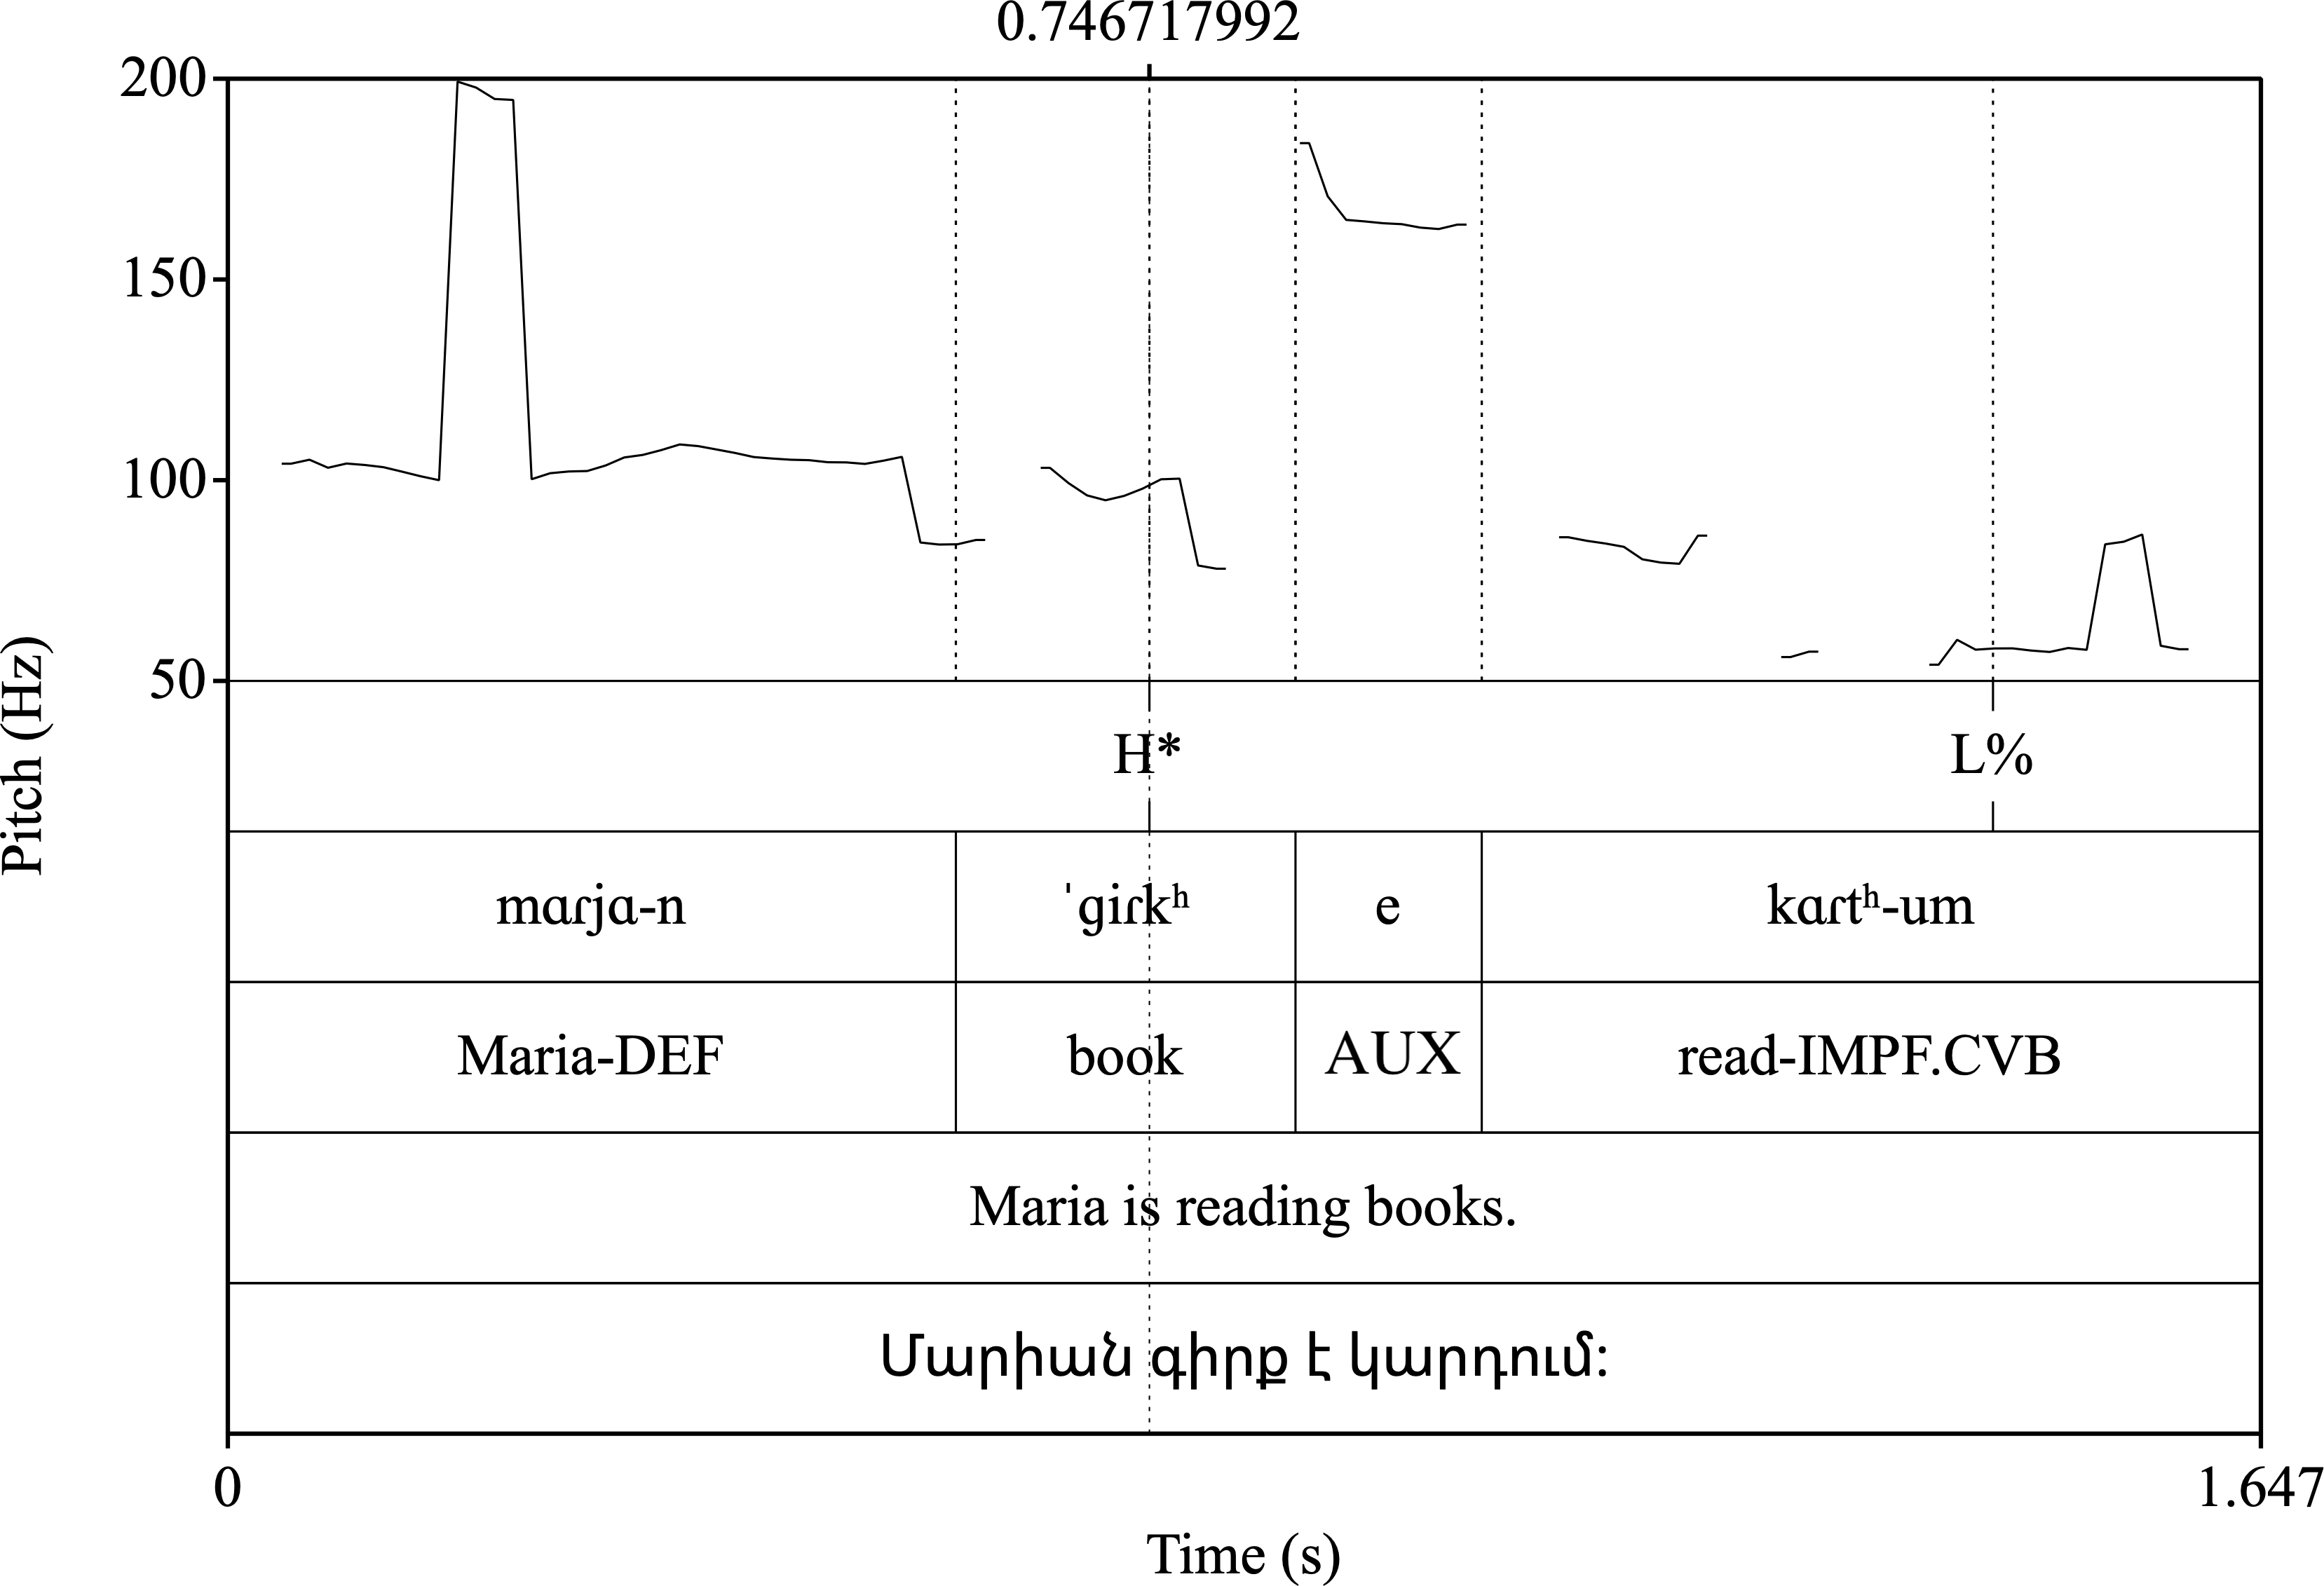
\includegraphics[width=\linewidth]{images/AT_Declarative.png}
			\caption{{\seaAbbre} declarative   with L\%}
		\end{subfigure}%
		\begin{subfigure}[b]{0.5\textwidth}
			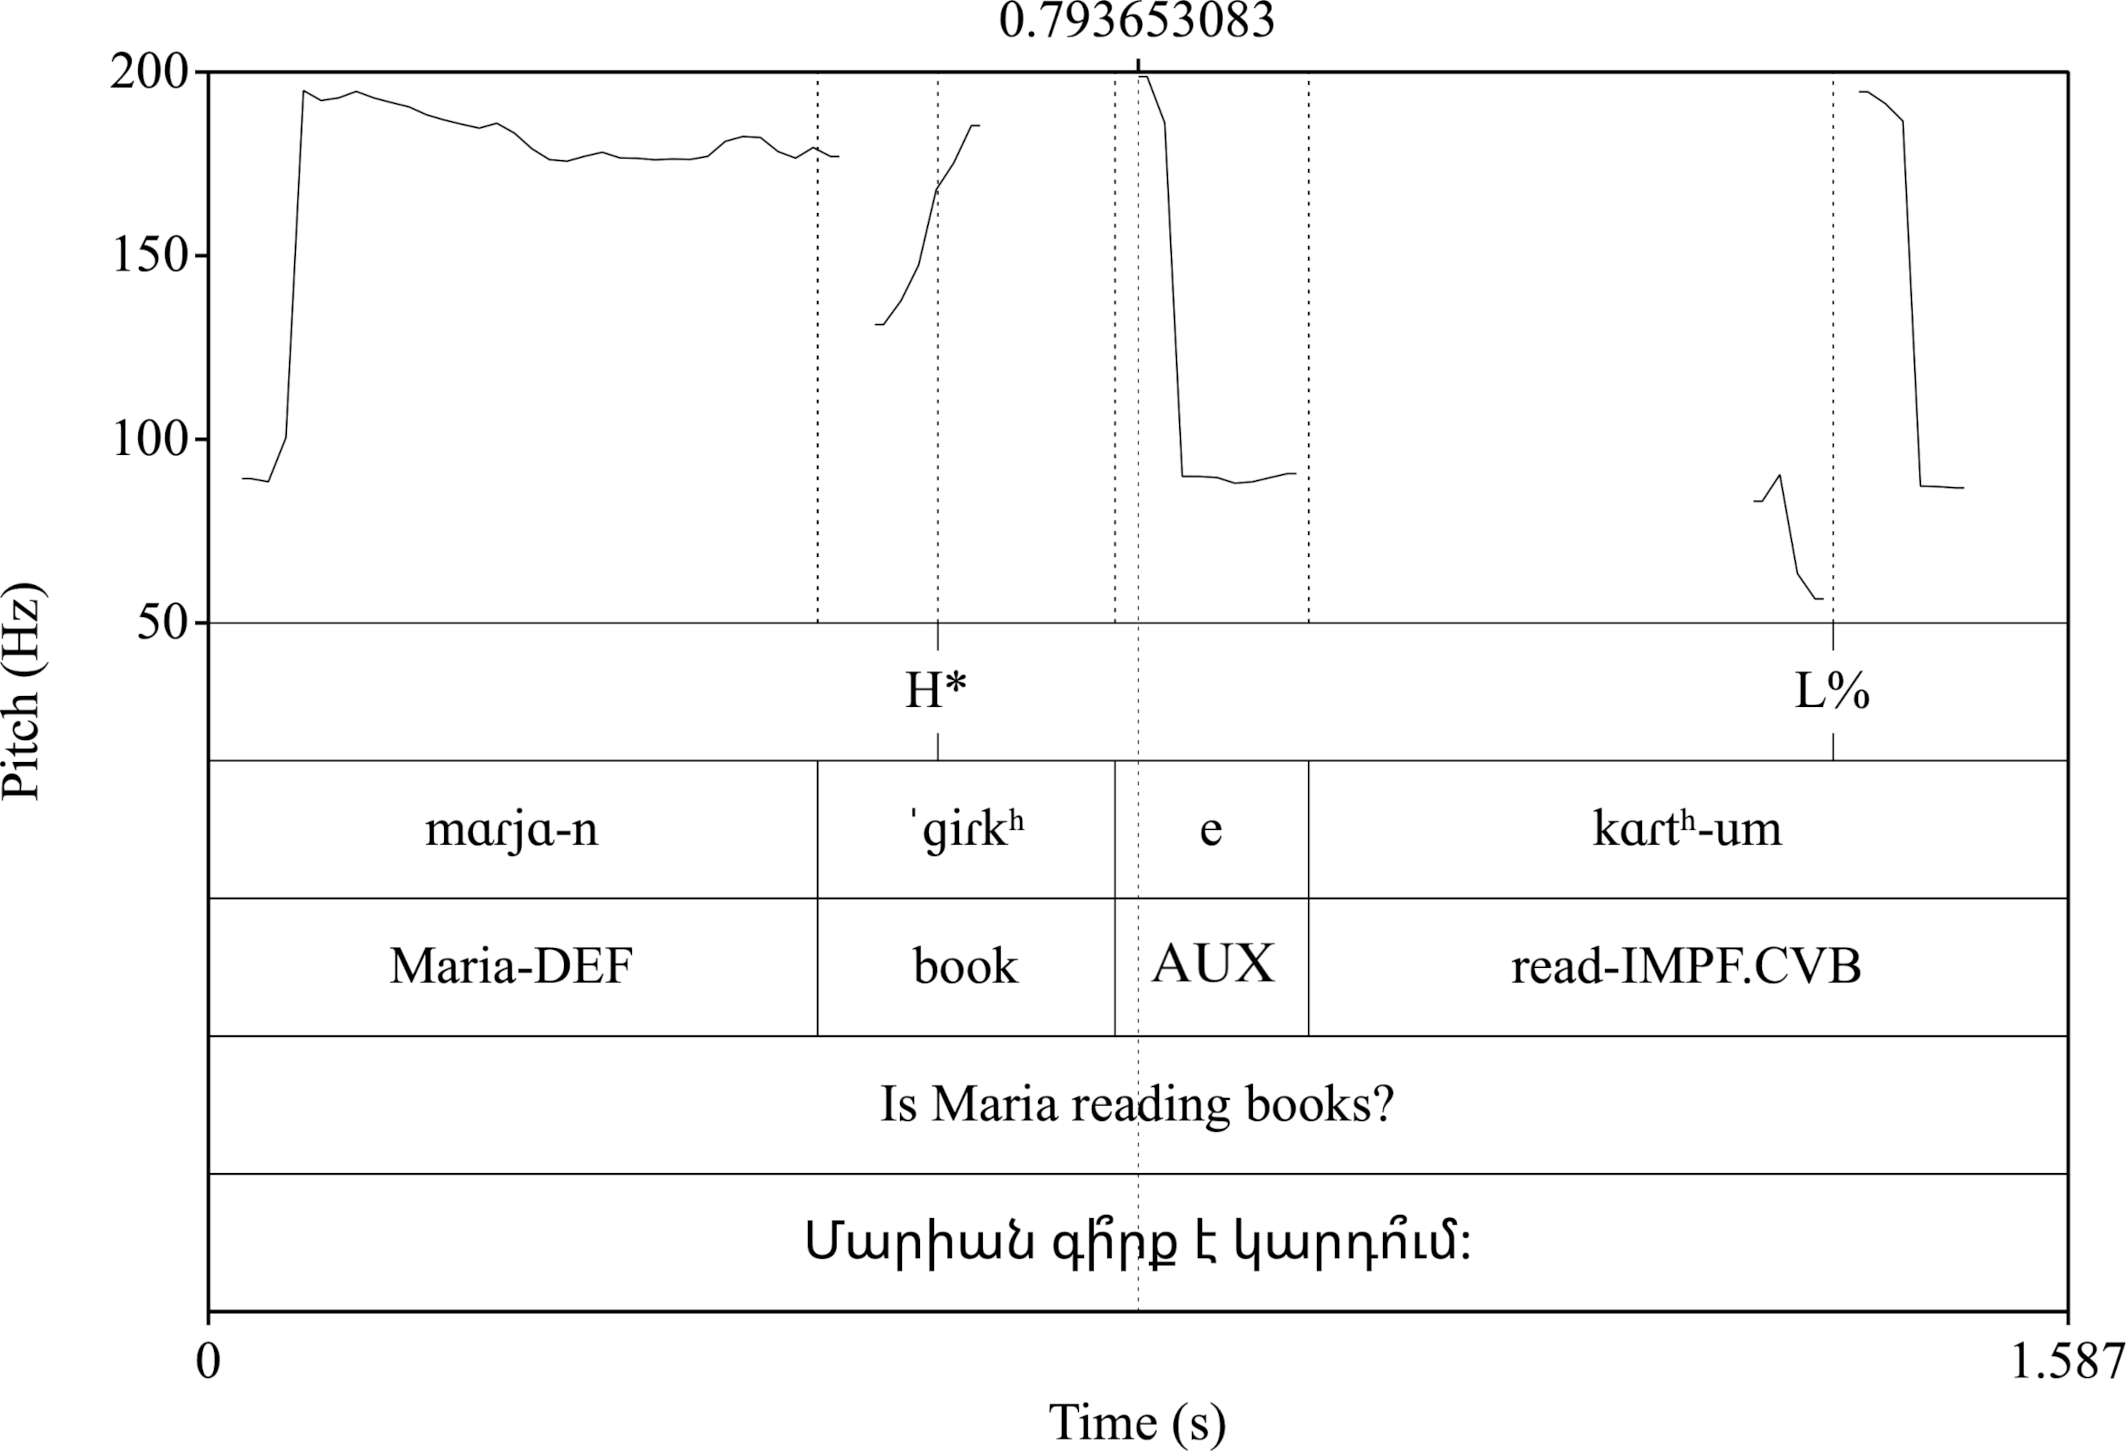
\includegraphics[width=\linewidth]{images/AT_PolarQuestion_LowTone.png}
			\caption{{\seaAbbre} polar  with L\%}
		\end{subfigure}\smallskip\\
		\begin{subfigure}[b]{0.5\textwidth}
			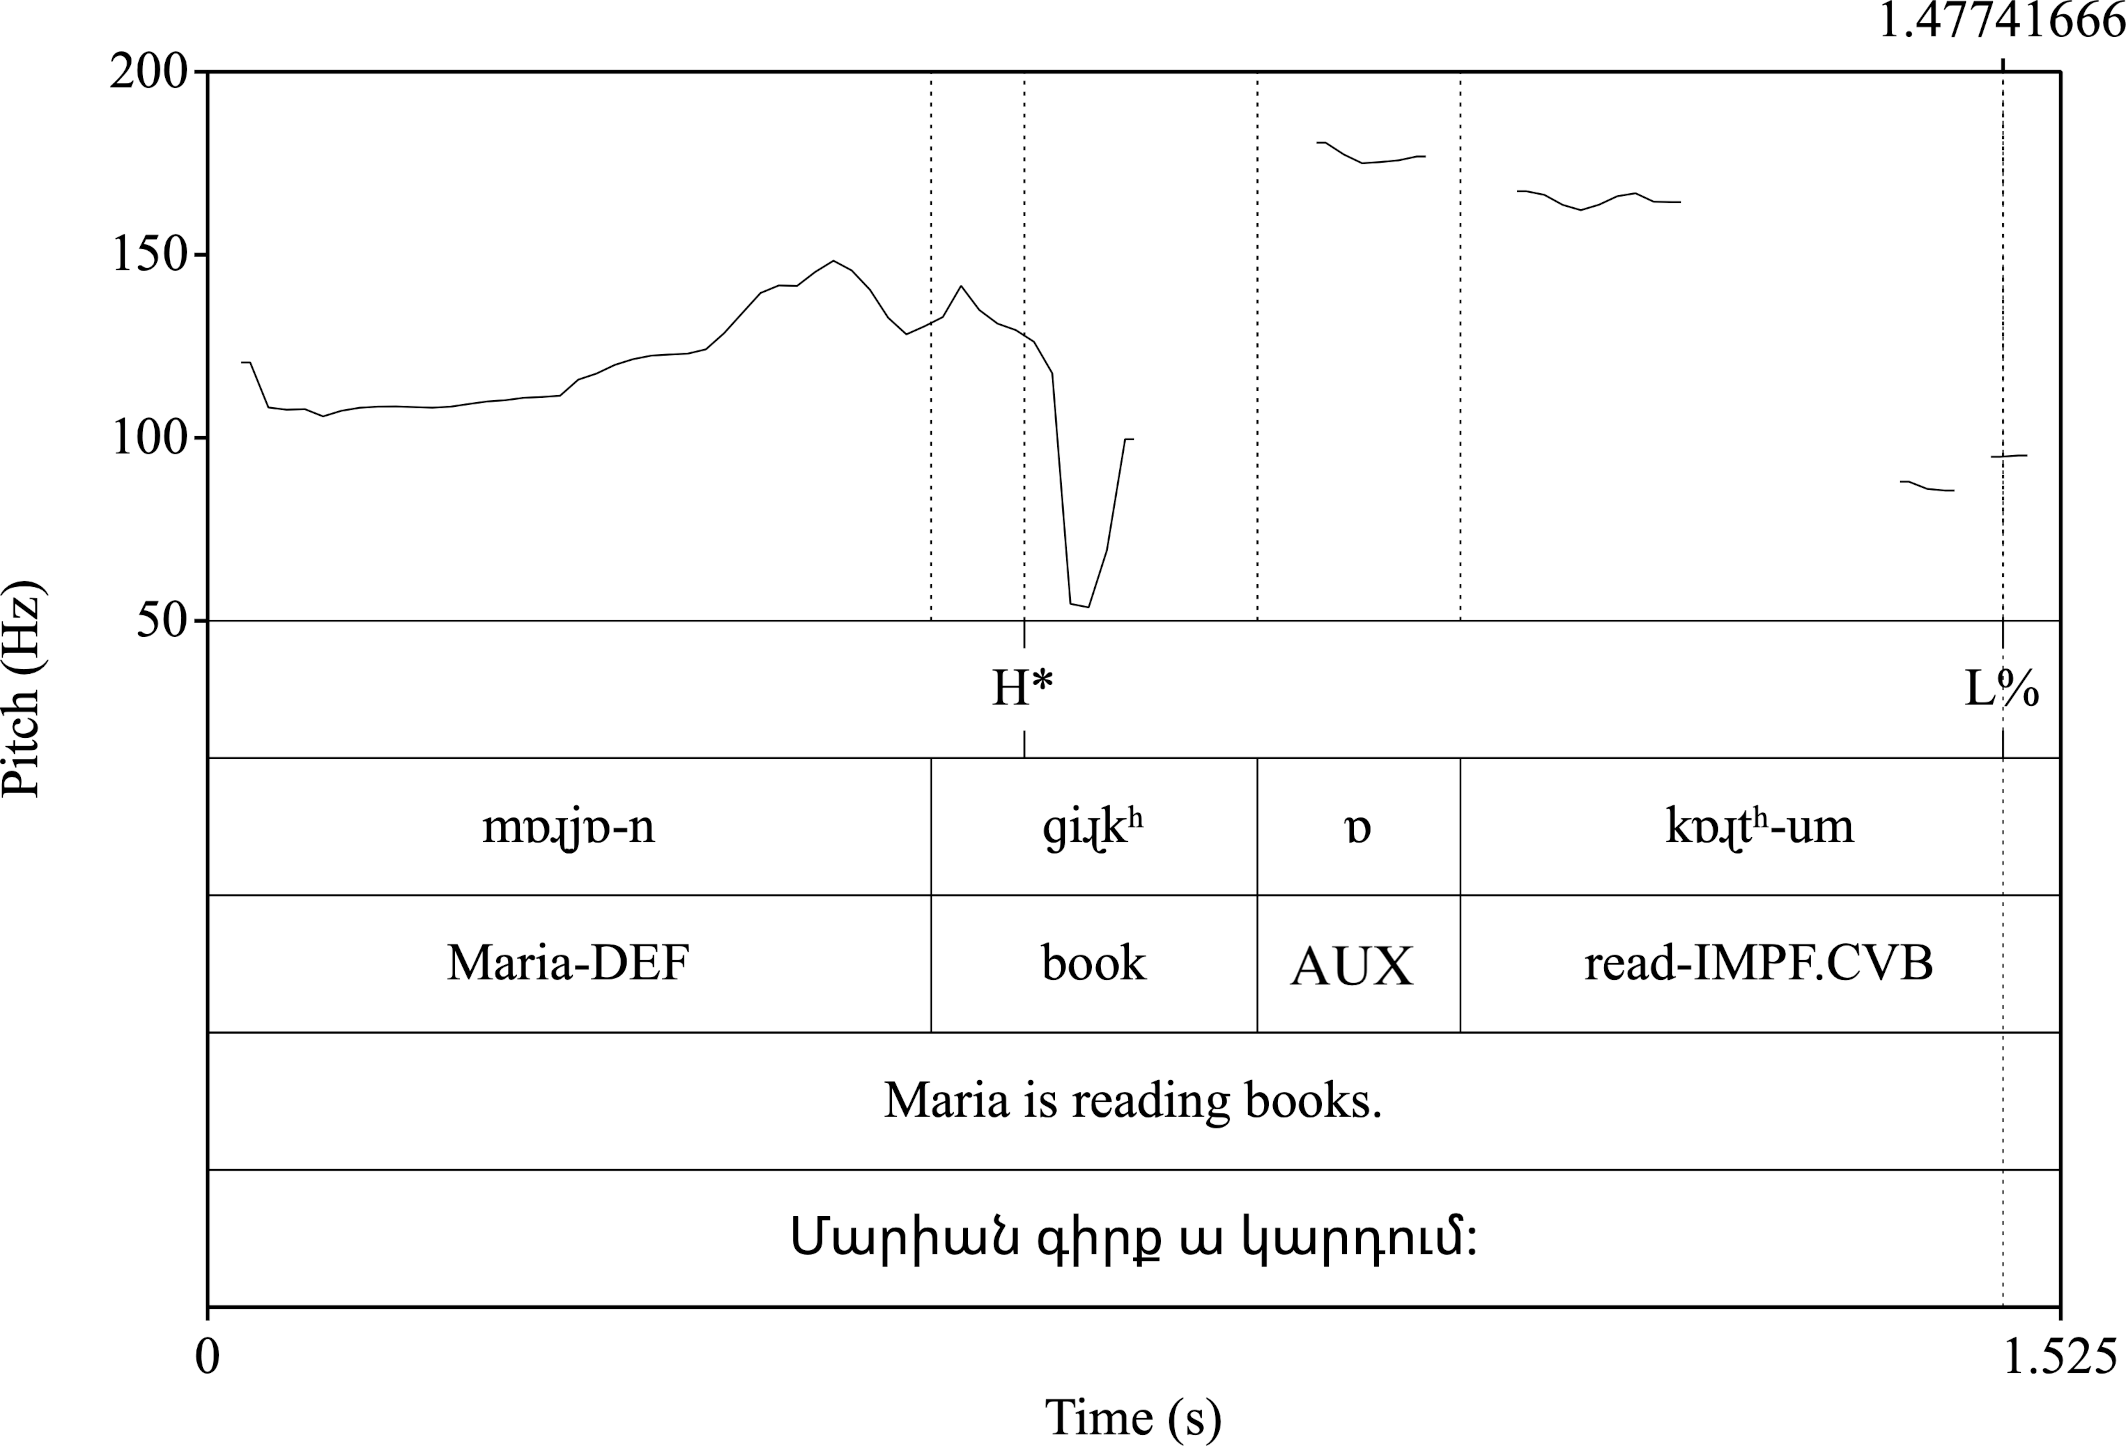
\includegraphics[width=\linewidth]{images/NK_Declarative.png}
			\caption{{\iaAbbre} declarative   with L\%}
		\end{subfigure}%
		\begin{subfigure}[b]{0.5\textwidth}
			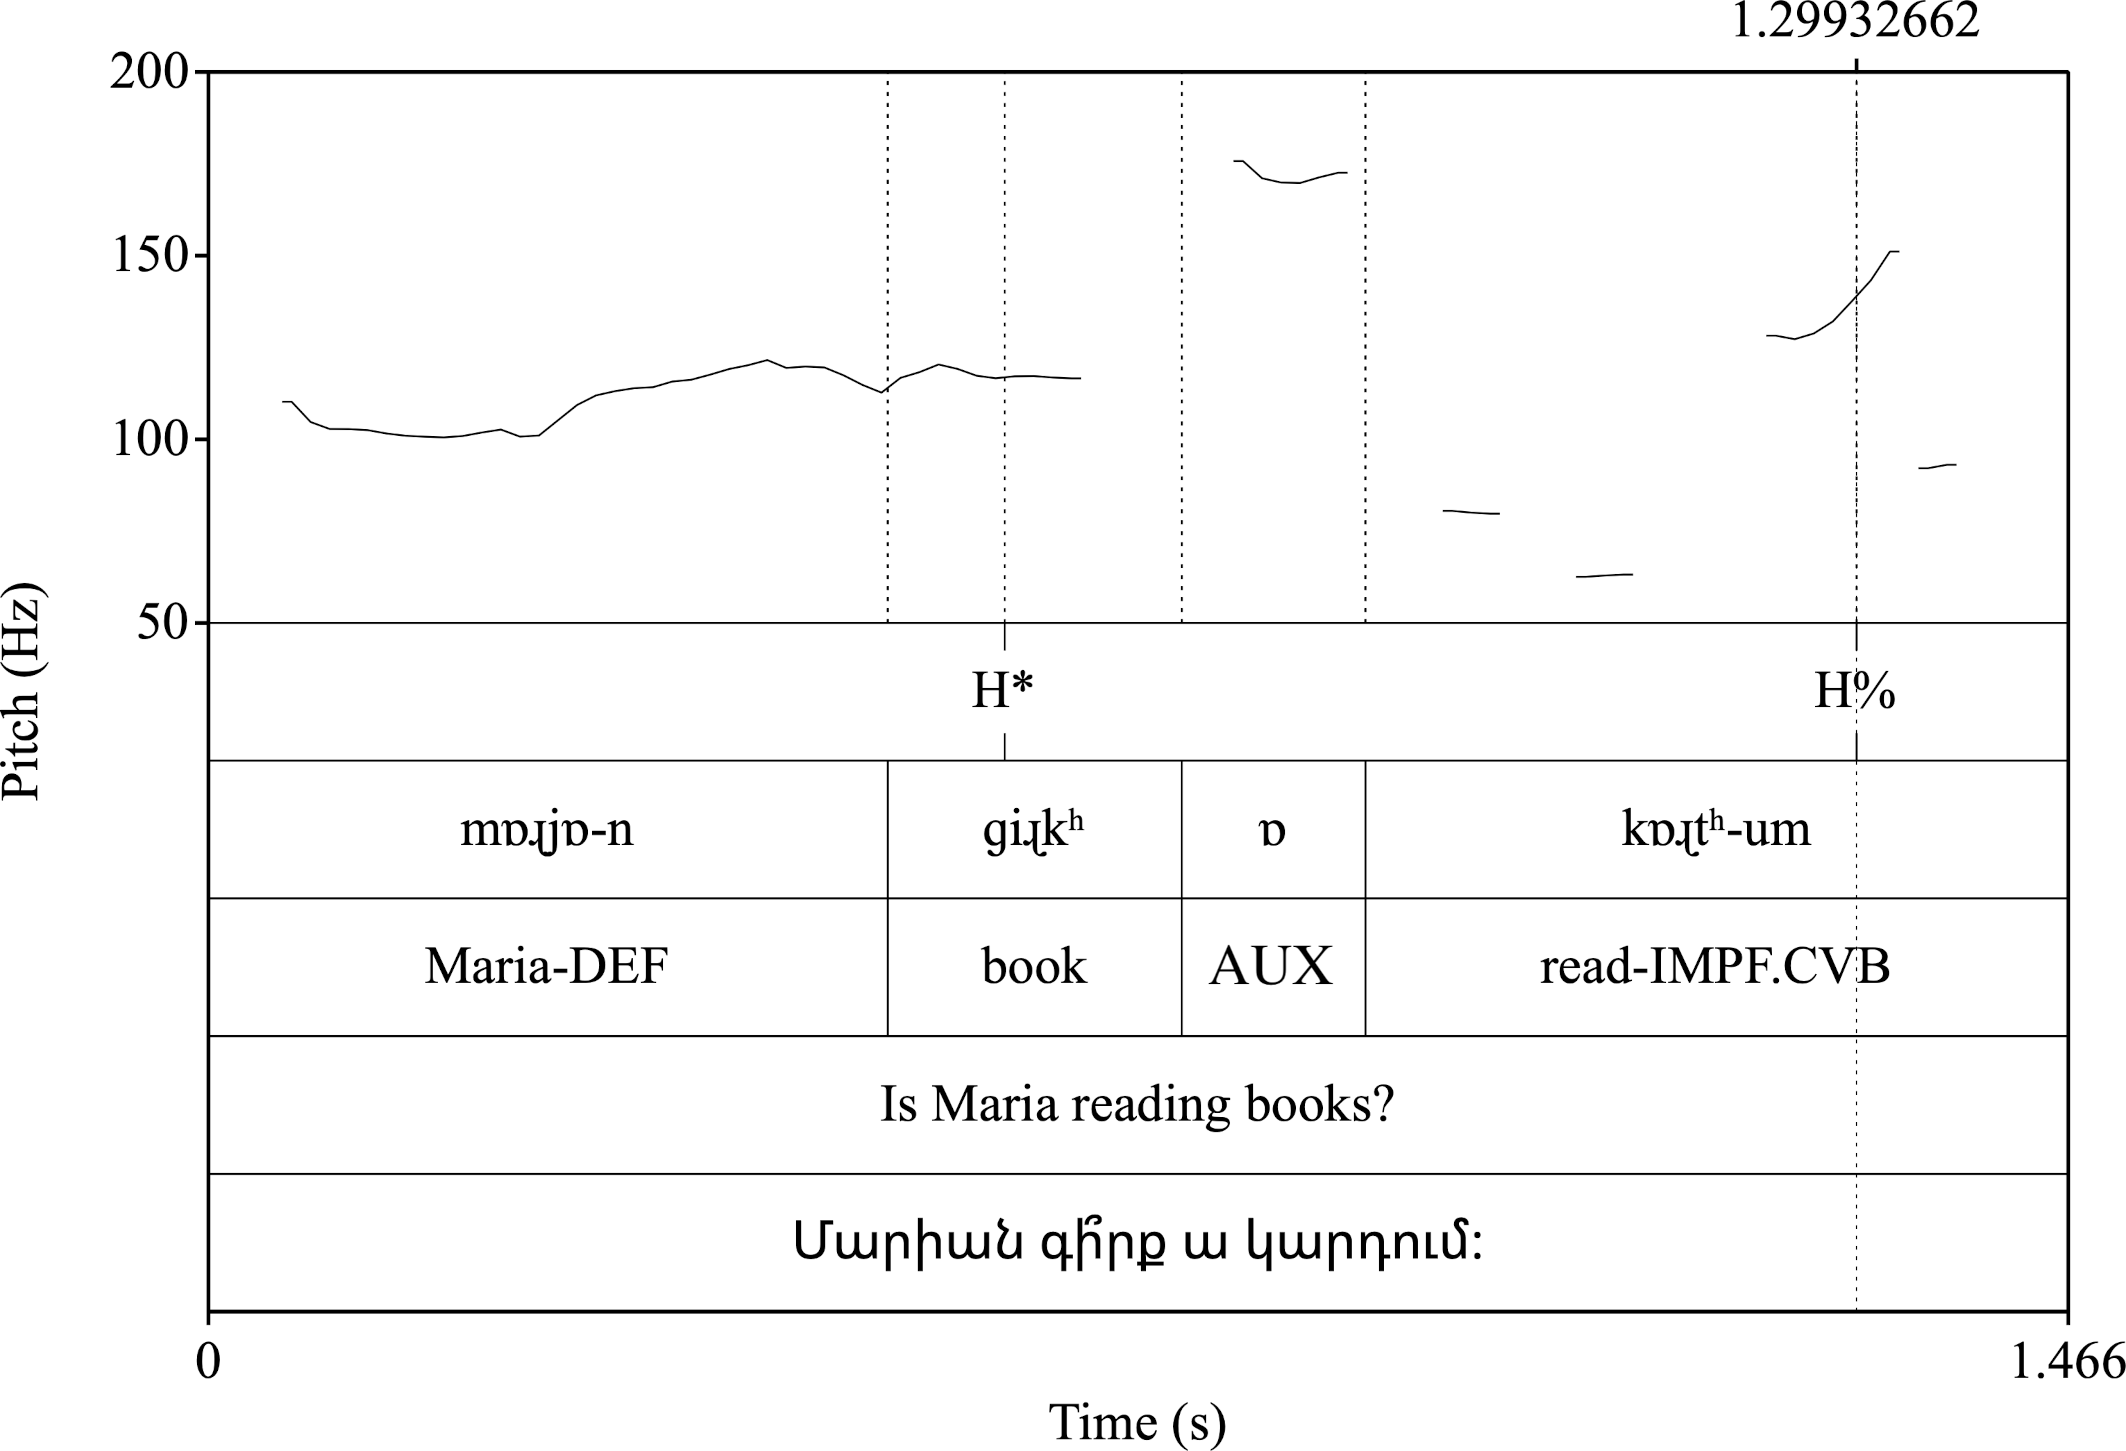
\includegraphics[width=\linewidth]{images/NK_PolarQuestion.png}
			\caption{{\iaAbbre} polar  with H\%}
		\end{subfigure}			
	\end{figure}\vfill\pagebreak
		
		The use of a sentence-final rise is likely due to two factors: one language-internal, and the other is language contact with Persian.
		
		
		In  Persian, polar questions end in a sentence-final rise as a type of Intonational Phrase boundary H\% (\citealt[111]{SadatTehrani-2007-IntonationPersian,sadat-2011-intonationPatternsInterrogativesPersian}, \citealt[55]{Mahjani-2003-PersianIntonation}). Furthermore, AS reports that some {\iaIA} speakers draw out the last syllable, i.e., they apply sentence-final lengthening. This is also reported in Persian polar questions \citep[113]{sadat-2011-intonationPatternsInterrogativesPersian}. 
		
 
		As for language-internal factors, prescriptively, {\seaSEA} uses L\% for polar questions when nuclear stress is on a non-final word. However, AT informs us that {\seaCEA} (as spoken in Yerevan) does allow a final H\%. She said that the use of this H\% is socially judged   as ``improper'' for her {\seaEA} community. We provide a pitch track in Figure \ref{fig:eastern polar H}. Another parallelism is that {\seaCEA} can also use the colloquial auxiliary [ɑ] (like {\iaAbbre}) instead of the standard [e]. 
		
 
		
		\begin{figure}
			\caption{Polar question in {\seaSE} (\ref{example: sov dec sentence}-i) with optional H\% }
			\label{fig:eastern polar H}
			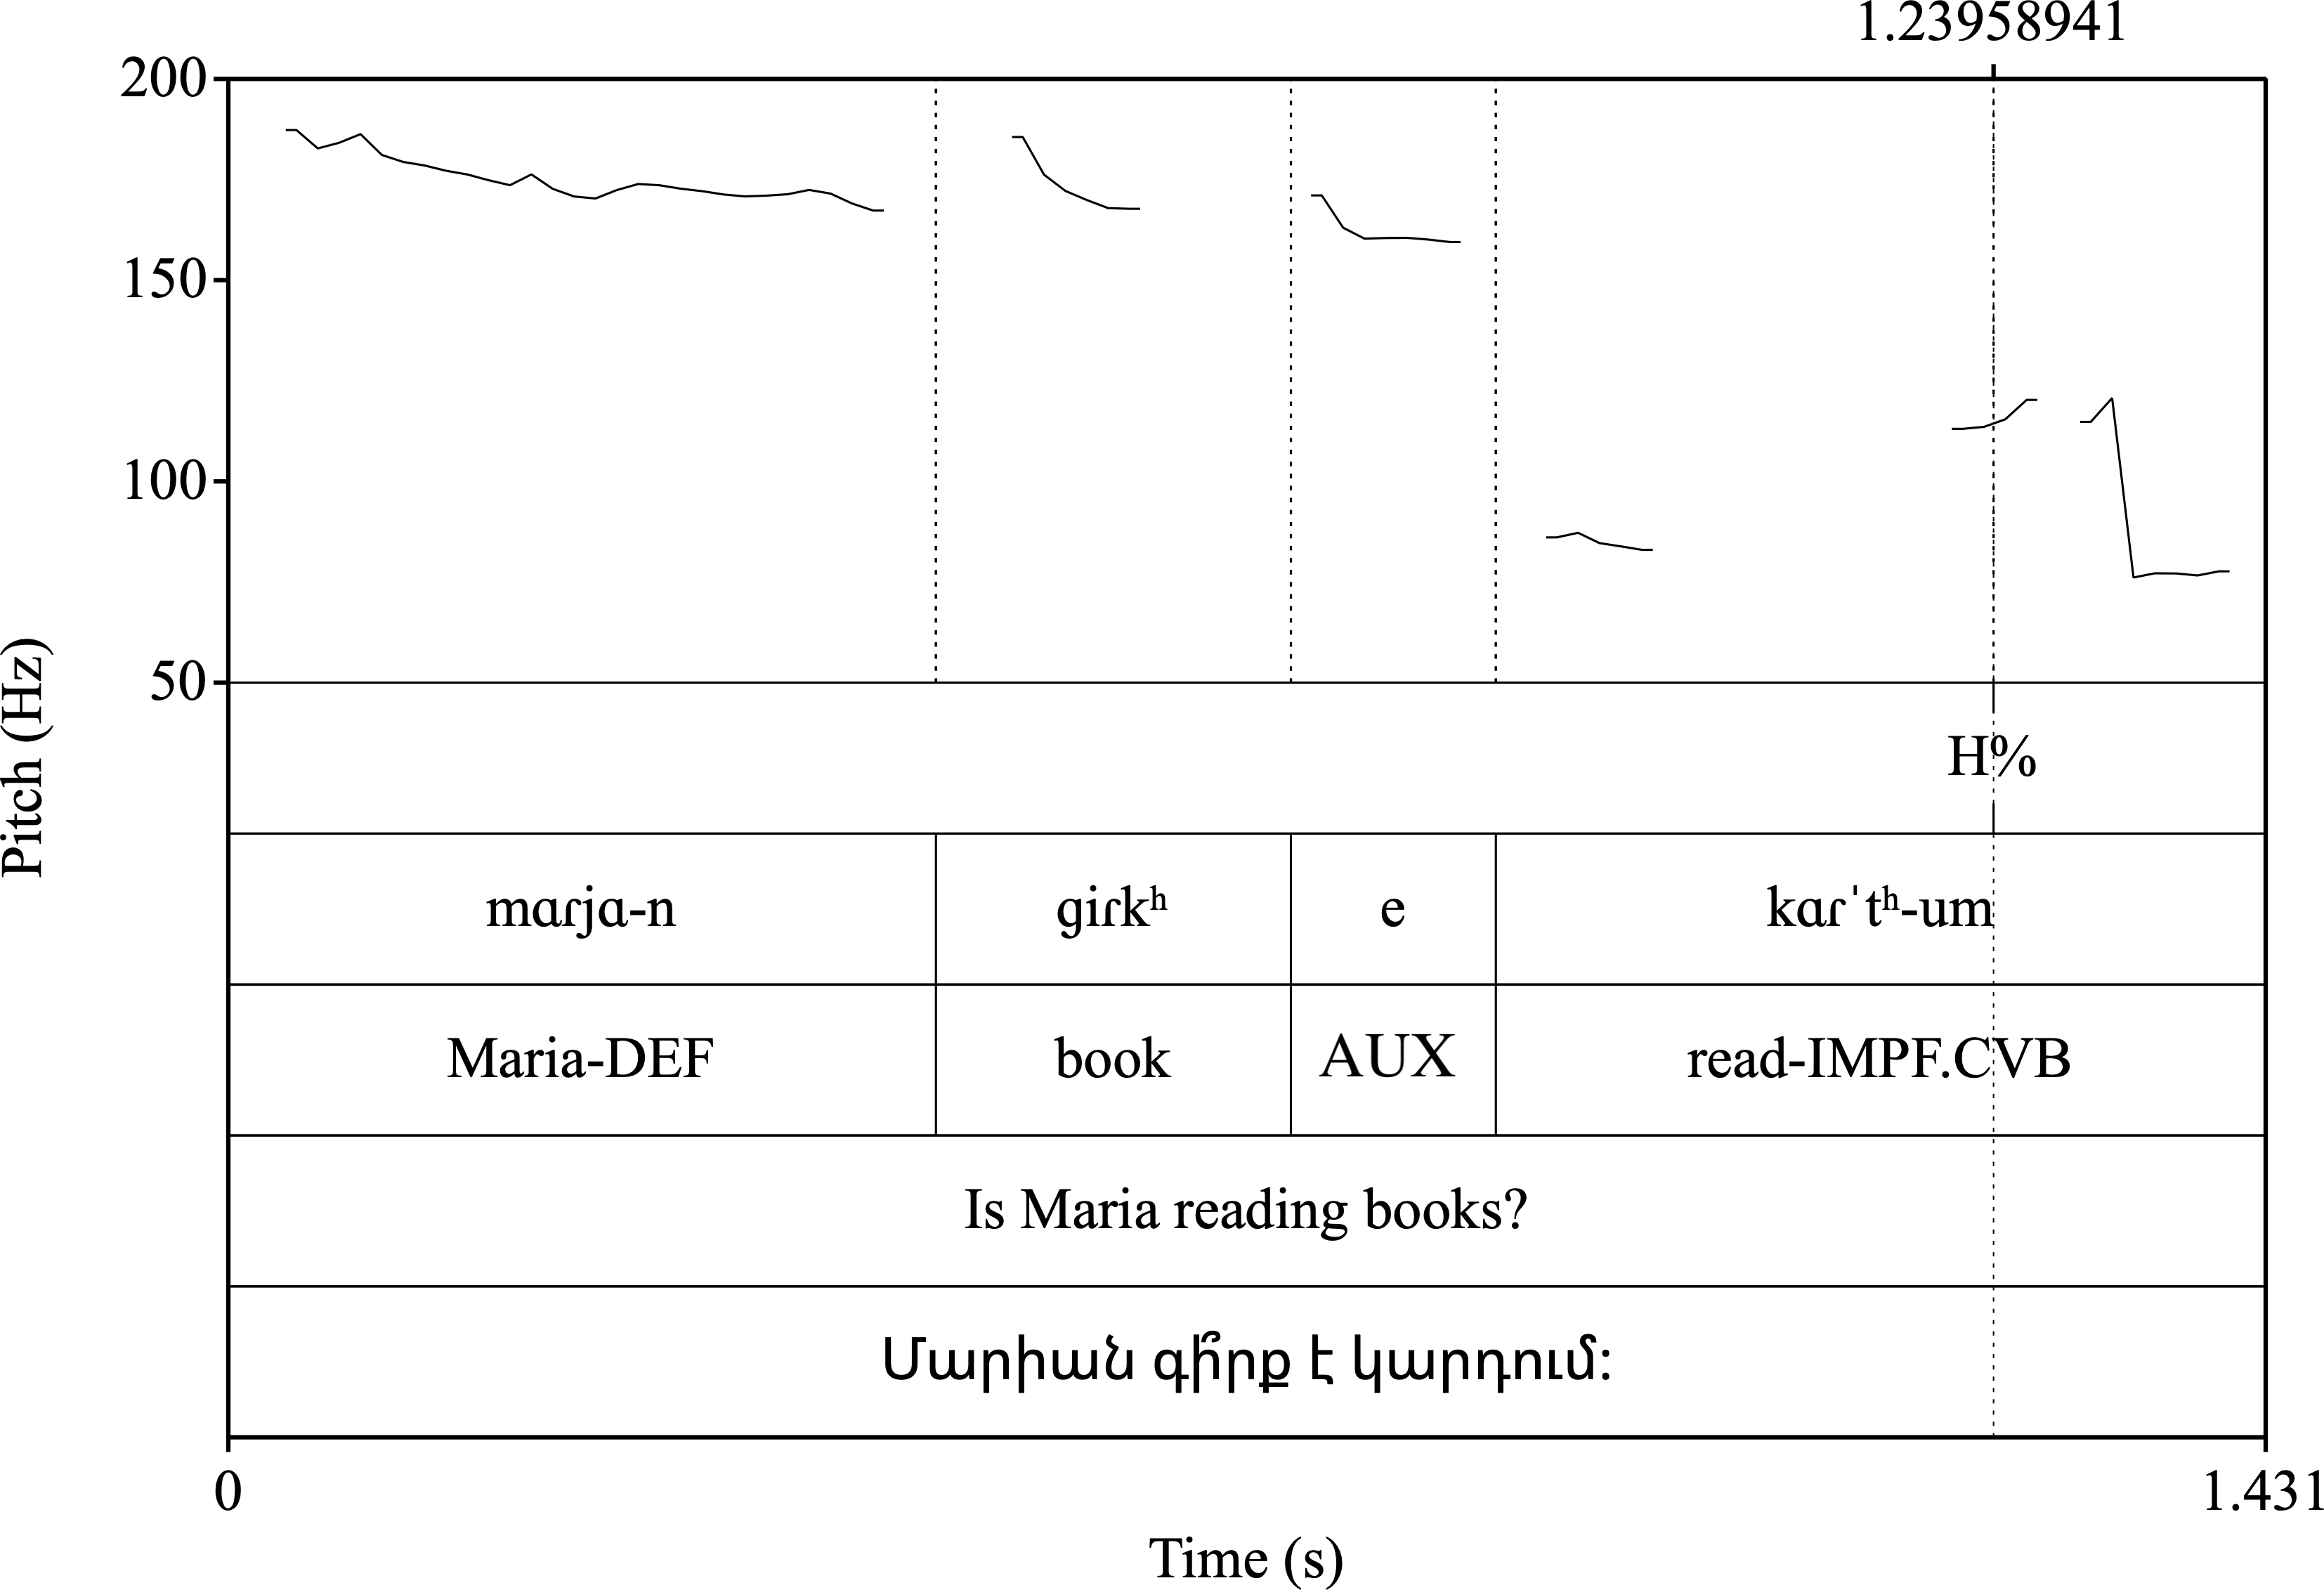
\includegraphics[scale= 0.6]{images/AT_PolarQuestion_HighTone.png}
		\end{figure}
		
		For {\iaIA}, the final syllable in a polar question can be considerably lengthened in order to indicate politeness. AS reports that final lengthening in {\iaIA} is common in order to indicate a non-aggressive and polite inquiry.
		
		Phonologically, the sentence-final H\% is on the final syllable of the polar question, regardless of whether that syllable carries lexical stress. 	For example, consider the following declarative sentence and its polar question form (\ref{example: v-aux dec sentence}). Morphologically, the sentence consists of a verb in a non-finite form, plus a   cliticized auxiliary. In the declarative, lexical stress and nuclear stress H* are on the last syllable of the verb, while the  clitic is unstressed and carries L\%. 
		
		
		\begin{exe}
			\ex 
			\begin{xlist}
				\ex \textit{Declarative    V-Aux with lexical stress on the V}\label{example: v-aux dec sentence}
				
				\begin{tabular}{l ll l}
					i.& {t͡sə\uline{χ-um}}  & ={e-s}$\searrow$&({\seaAbbre})
					\\
					ii.& {t͡sə\uline{χ-um}}  & ={e-s}$\searrow$&({\iaAbbre})
					\\
					& smoke-{\impfcvb} & {\auxgloss}-2{\sg} & \\
					&\multicolumn{3}{l}{`You smoke.'} 
					\\ 
					&\multicolumn{3}{l}{\armenian{Ծխում ես։}}
					\\
				\end{tabular} 
				\ex \textit{Polar question} \label{example: v-aux polar sentence}
				
				\begin{tabular}{llll}
					i.& {t͡sə\uline{χ-um}}$\nearrow$  & ={e-s}$\searrow$&({\seaAbbre})
					\\
					ii. &  {t͡səχ-um} &  ={e-s}$\nearrow$ &   ({\iaAbbre})
					\\
					& smoke-{\impfcvb} & {\auxgloss}-2{\sg} & \\
					& \multicolumn{3}{l}{`Do you smoke?'}
					\\
					&\multicolumn{3}{l}{\armenian{Ծխու՞մ ես։}}
					
					
				\end{tabular} 
				
			\end{xlist}
			
		\end{exe}
		
		
		In the polar form, the {\seaSE} version simply makes the nuclear stress more prominent, while the clitic keeps its L\% tone. But in {\iaIA}, sentence-final H\% is placed on the clitic. The proximity of H\% and the verb causes the verb to lose its nuclear stress.  	We show a pitch track for these sentences  in Figure \ref{fig:smoke pitch} from NK and AT.
		
		\begin{figure}
			\caption{Pitch track of declarative (\ref{example: v-aux dec sentence}) and polar question (\ref{example: v-aux polar sentence})   in {\seaAbbre}   and  {\iaAbbre} }
			\label{fig:smoke pitch}
			\begin{subfigure}[b]{0.5\textwidth}
				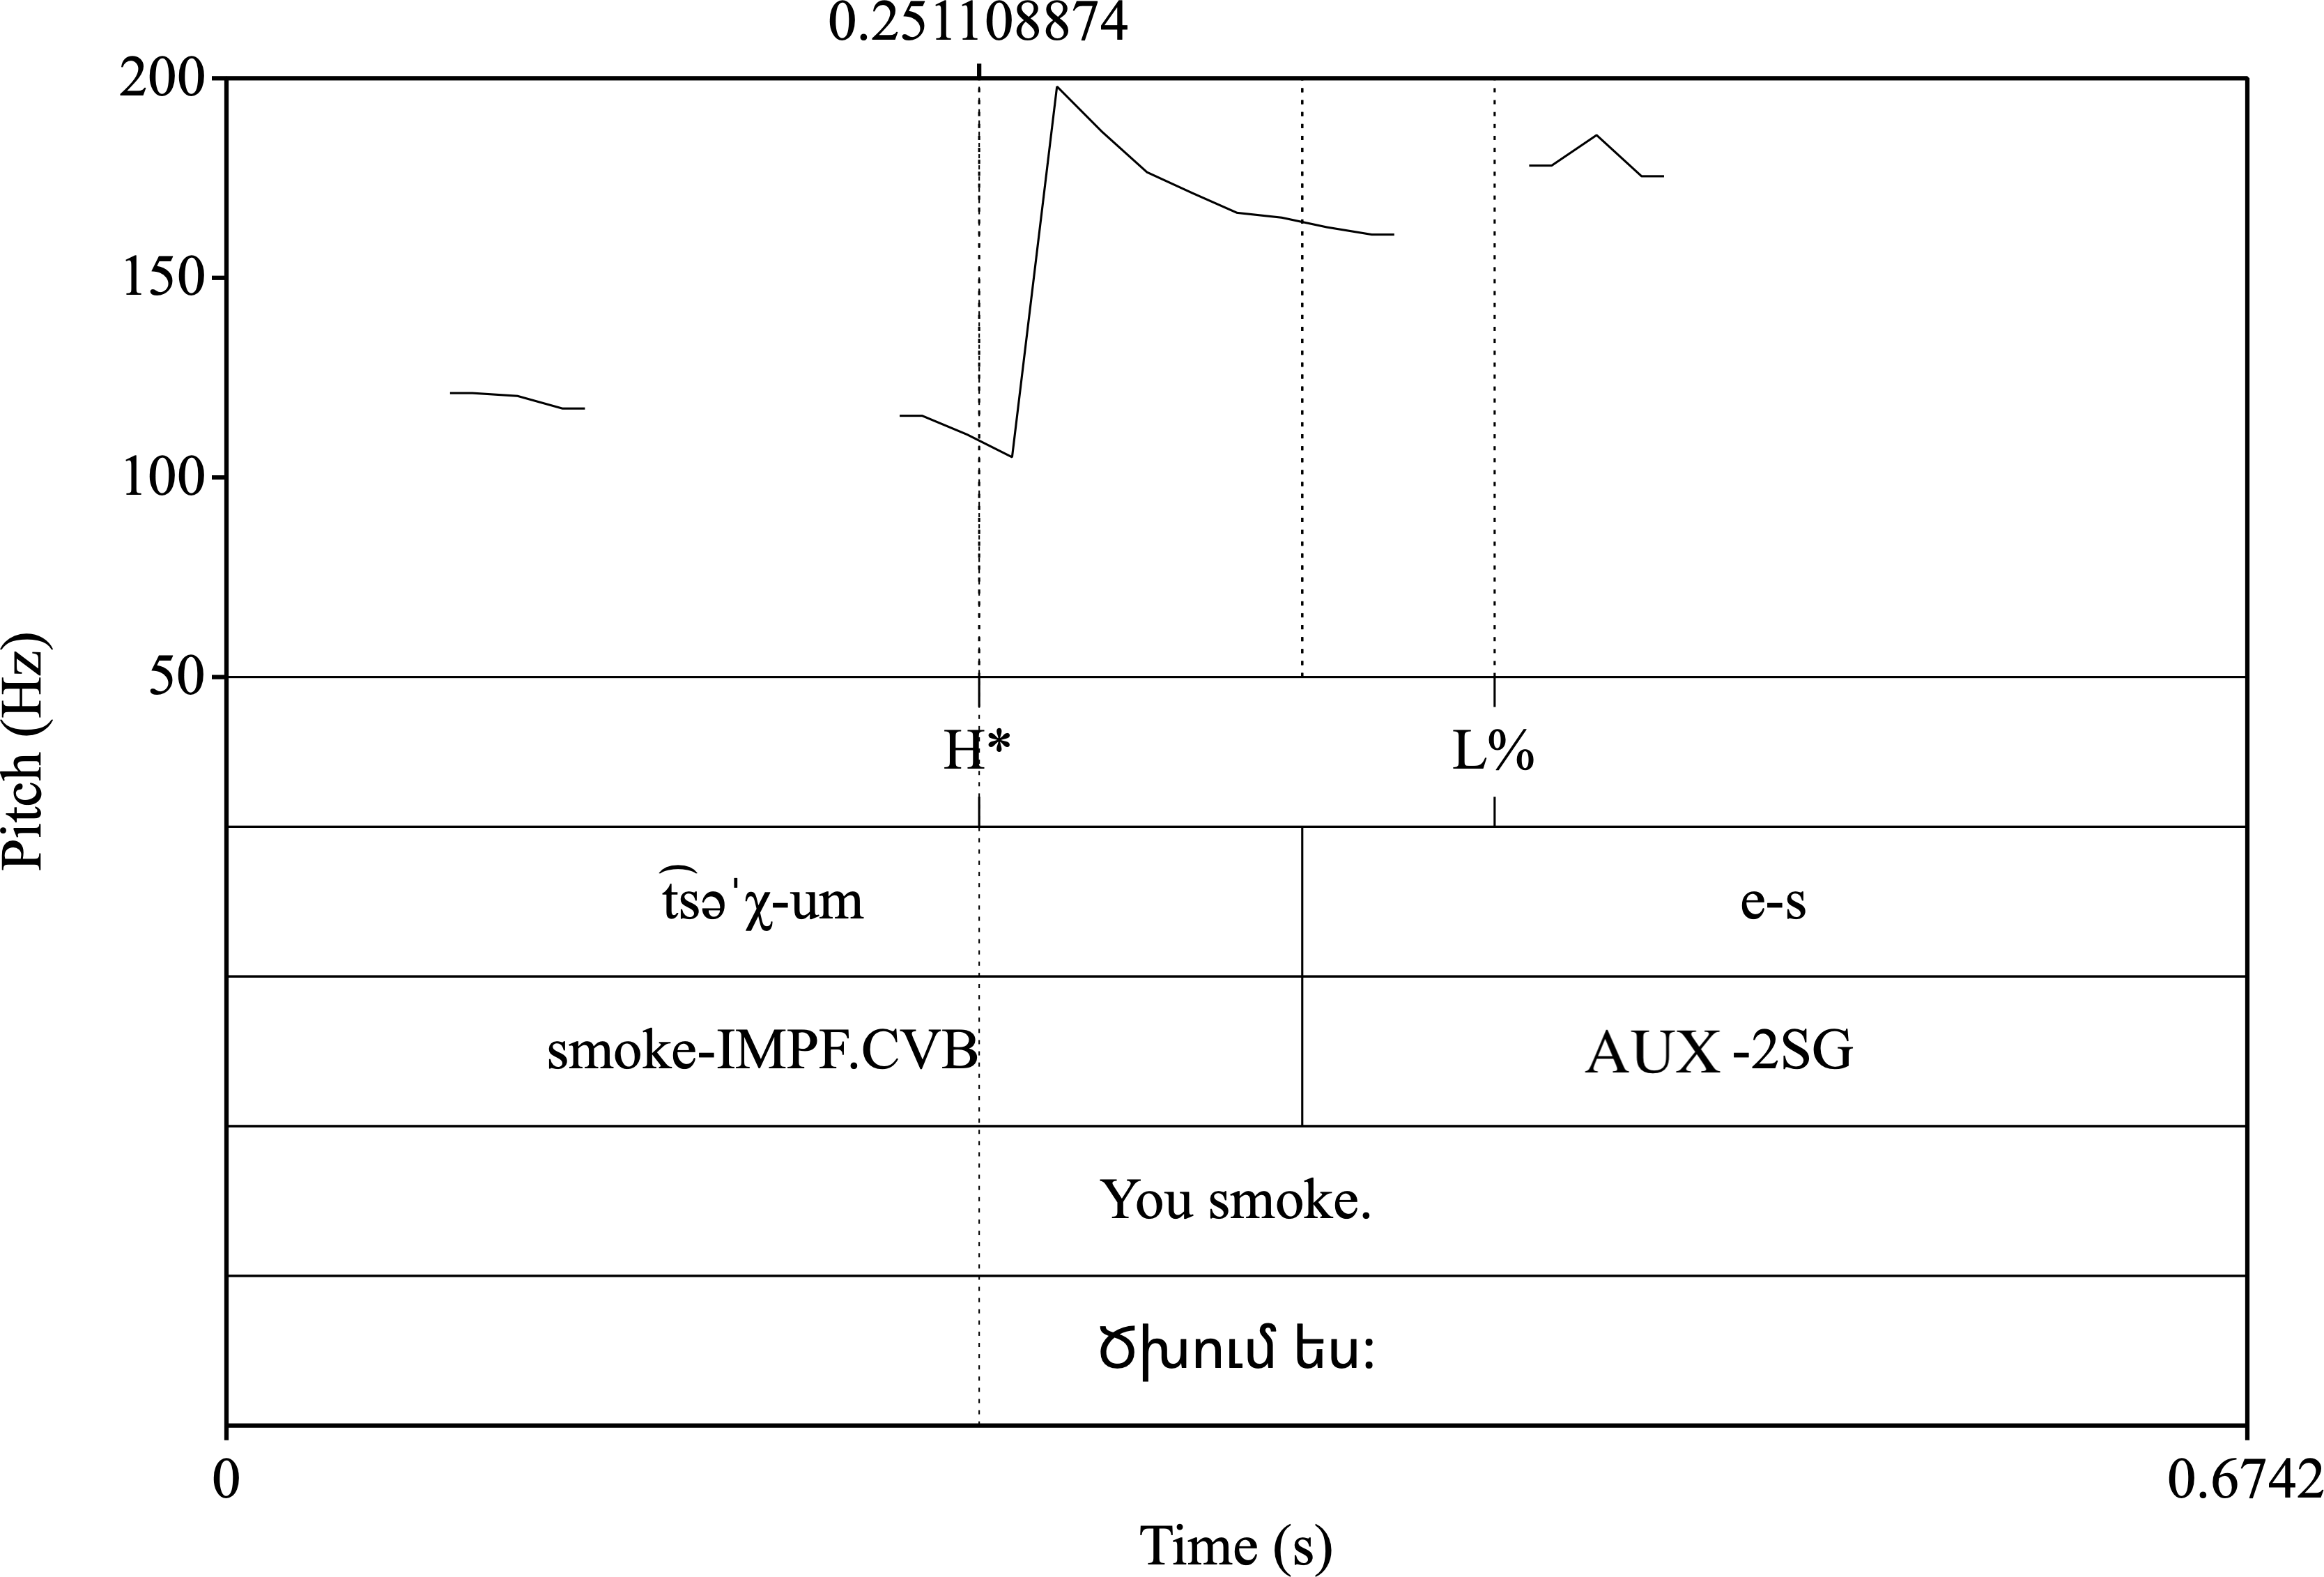
\includegraphics[width=\linewidth]{images/AT_Declarative_Clitic.png}
				\caption{{\seaAbbre} declarative   with L\%}
			\end{subfigure}%
			\begin{subfigure}[b]{0.5\textwidth}
				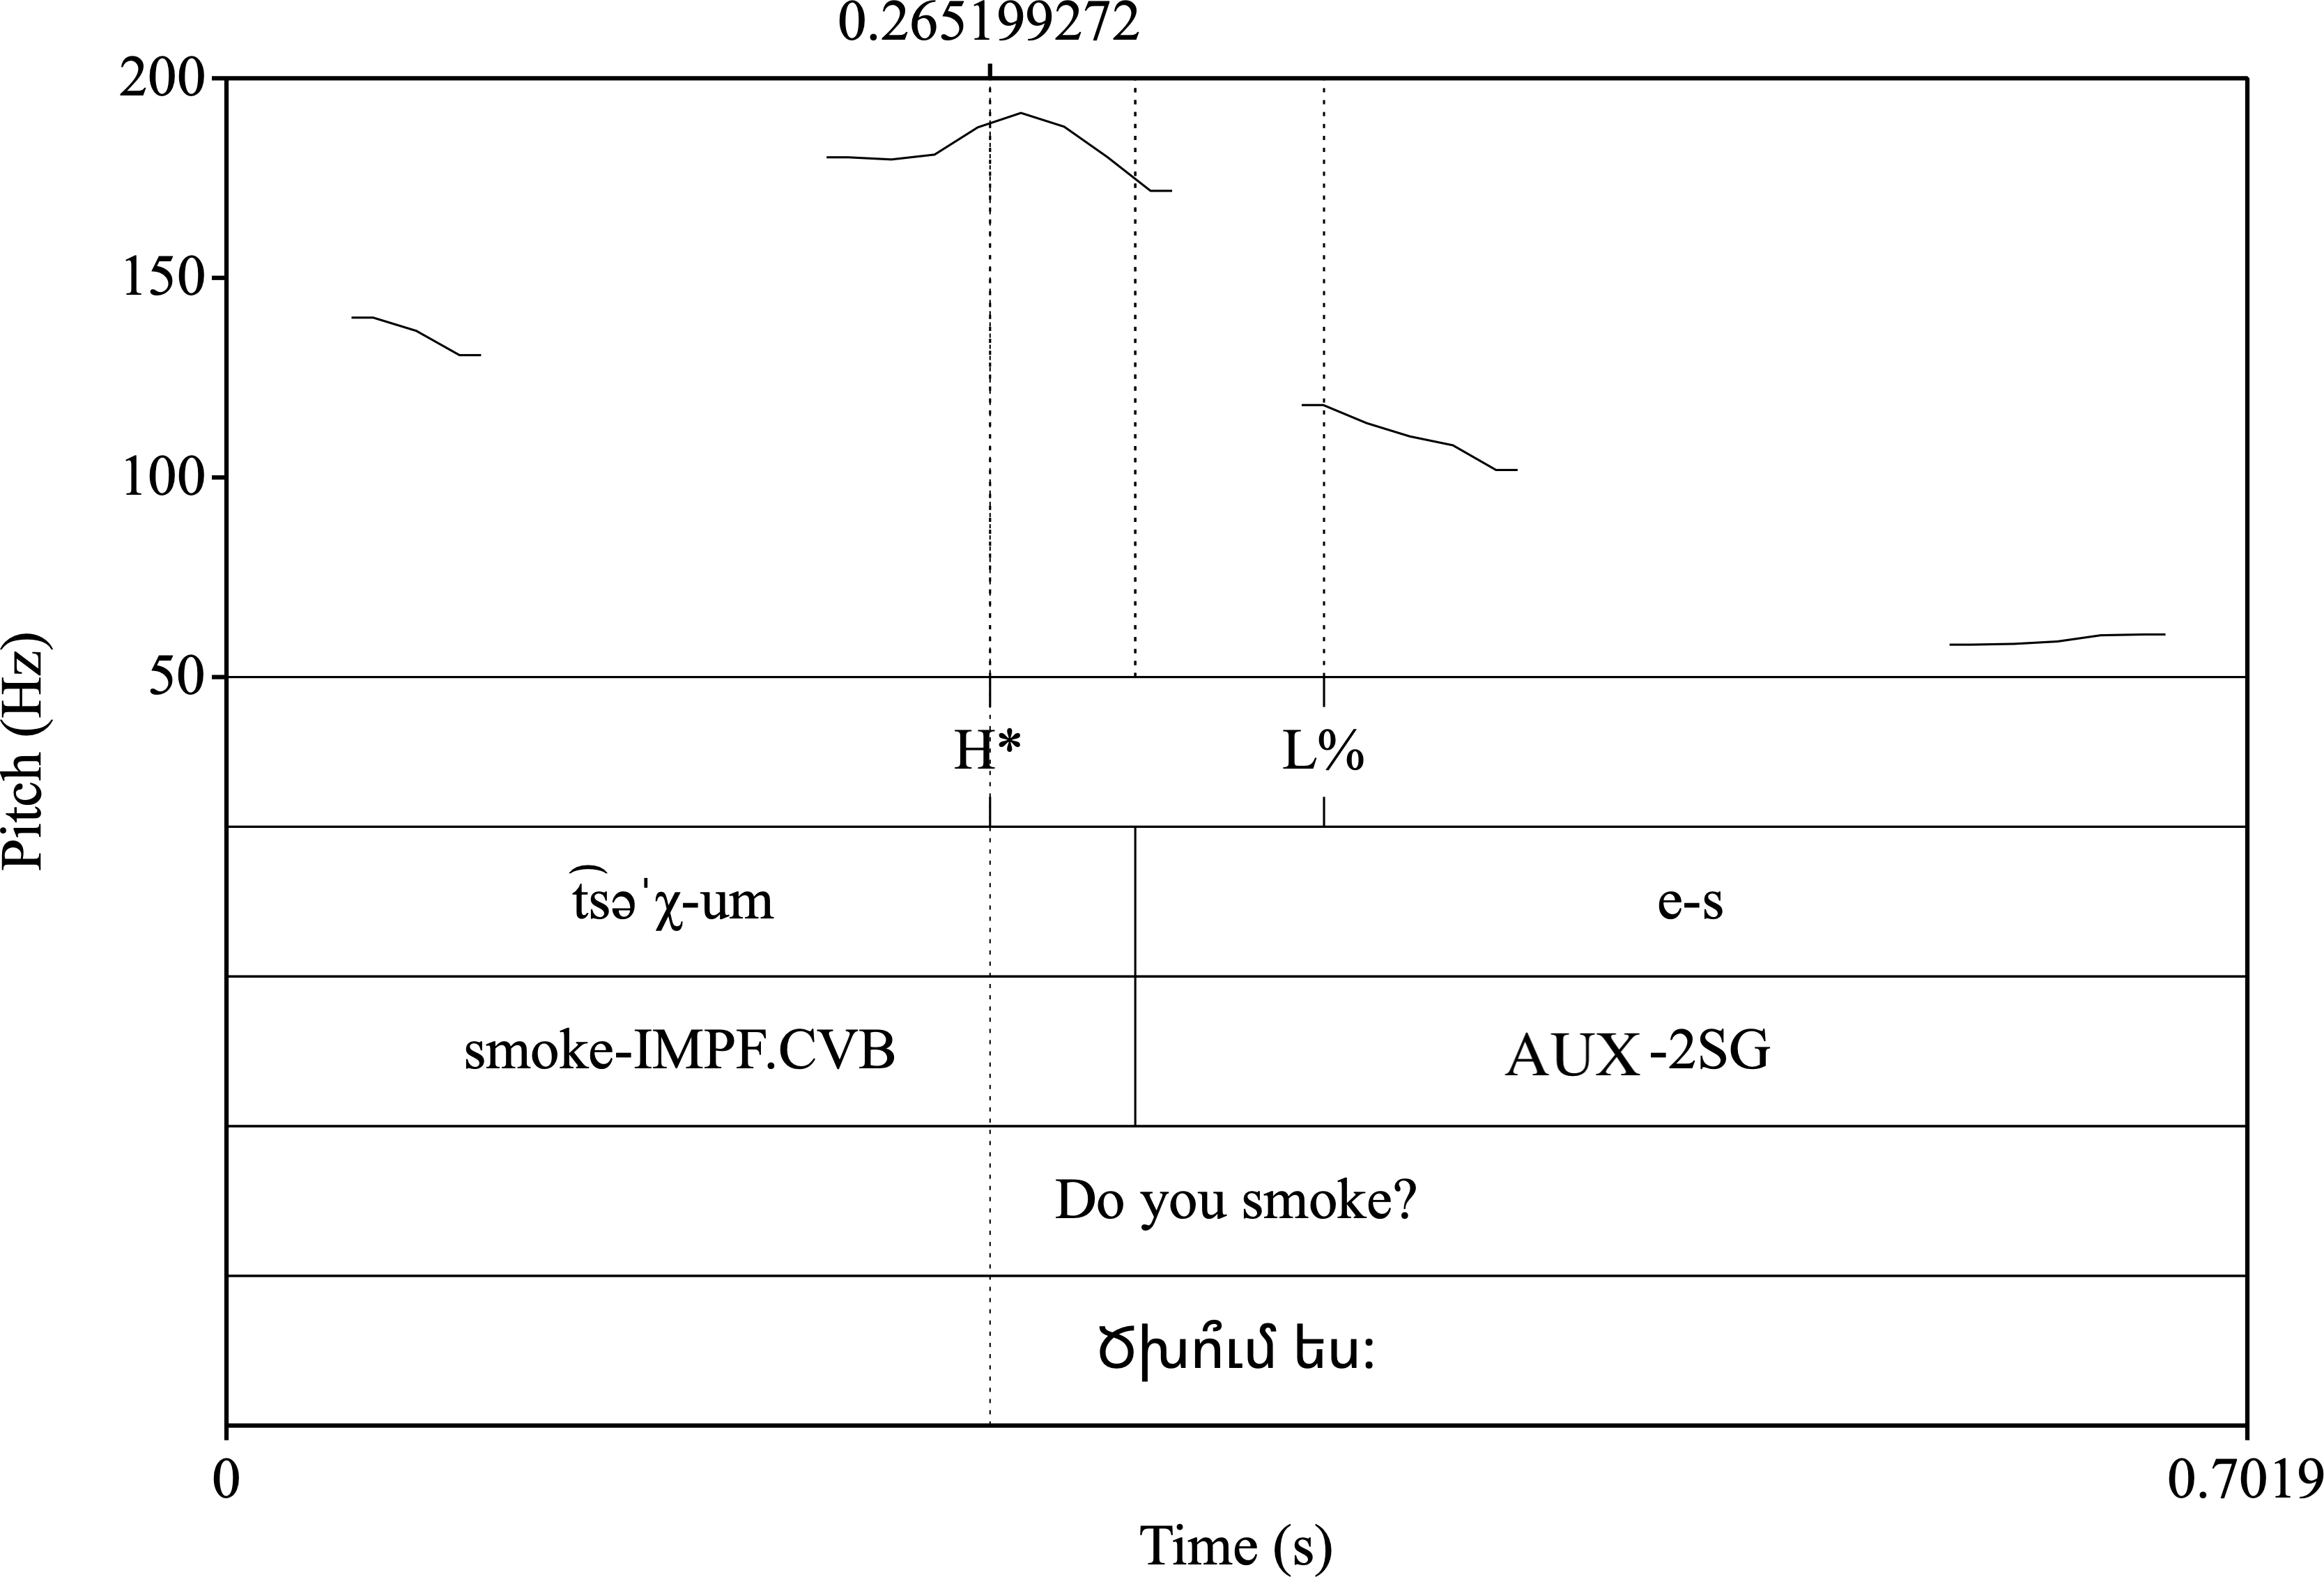
\includegraphics[width=\linewidth]{images/AT_PolarQuestion_Clitic.png}
				\caption{{\seaAbbre} polar  with L\%}
			\end{subfigure}\smallskip\\
			\begin{subfigure}[b]{0.5\textwidth}
				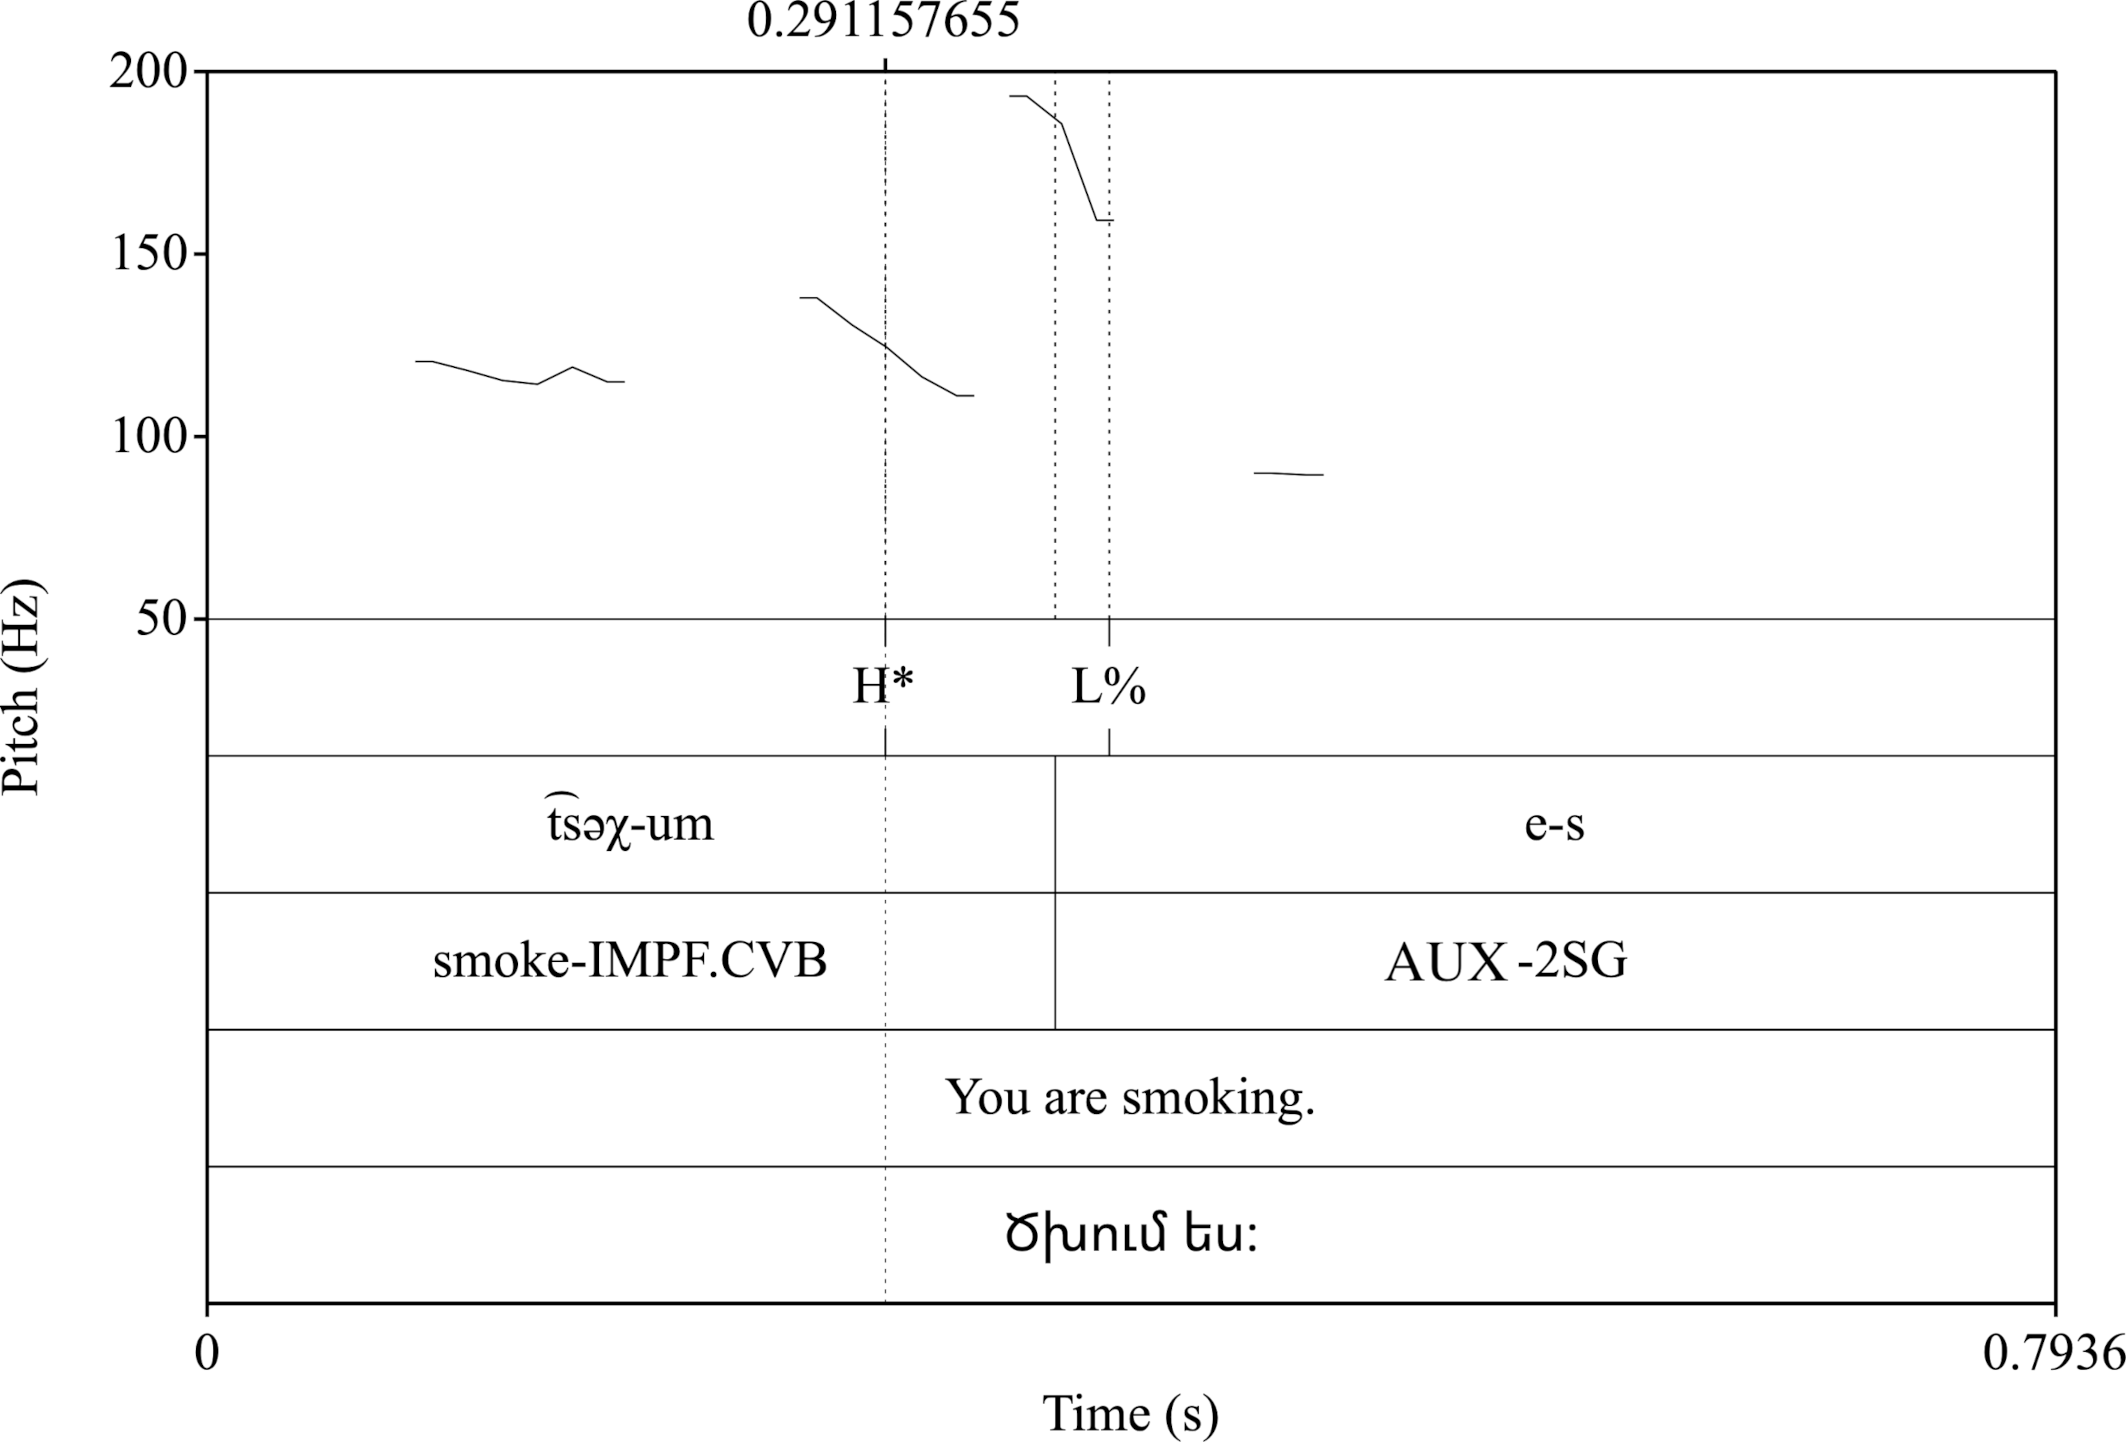
\includegraphics[width=\linewidth]{images/NK_Declarative_Clitic.png}
				\caption{{\iaAbbre} declarative   with L\%}
			\end{subfigure}%
			\begin{subfigure}[b]{0.5\textwidth}
				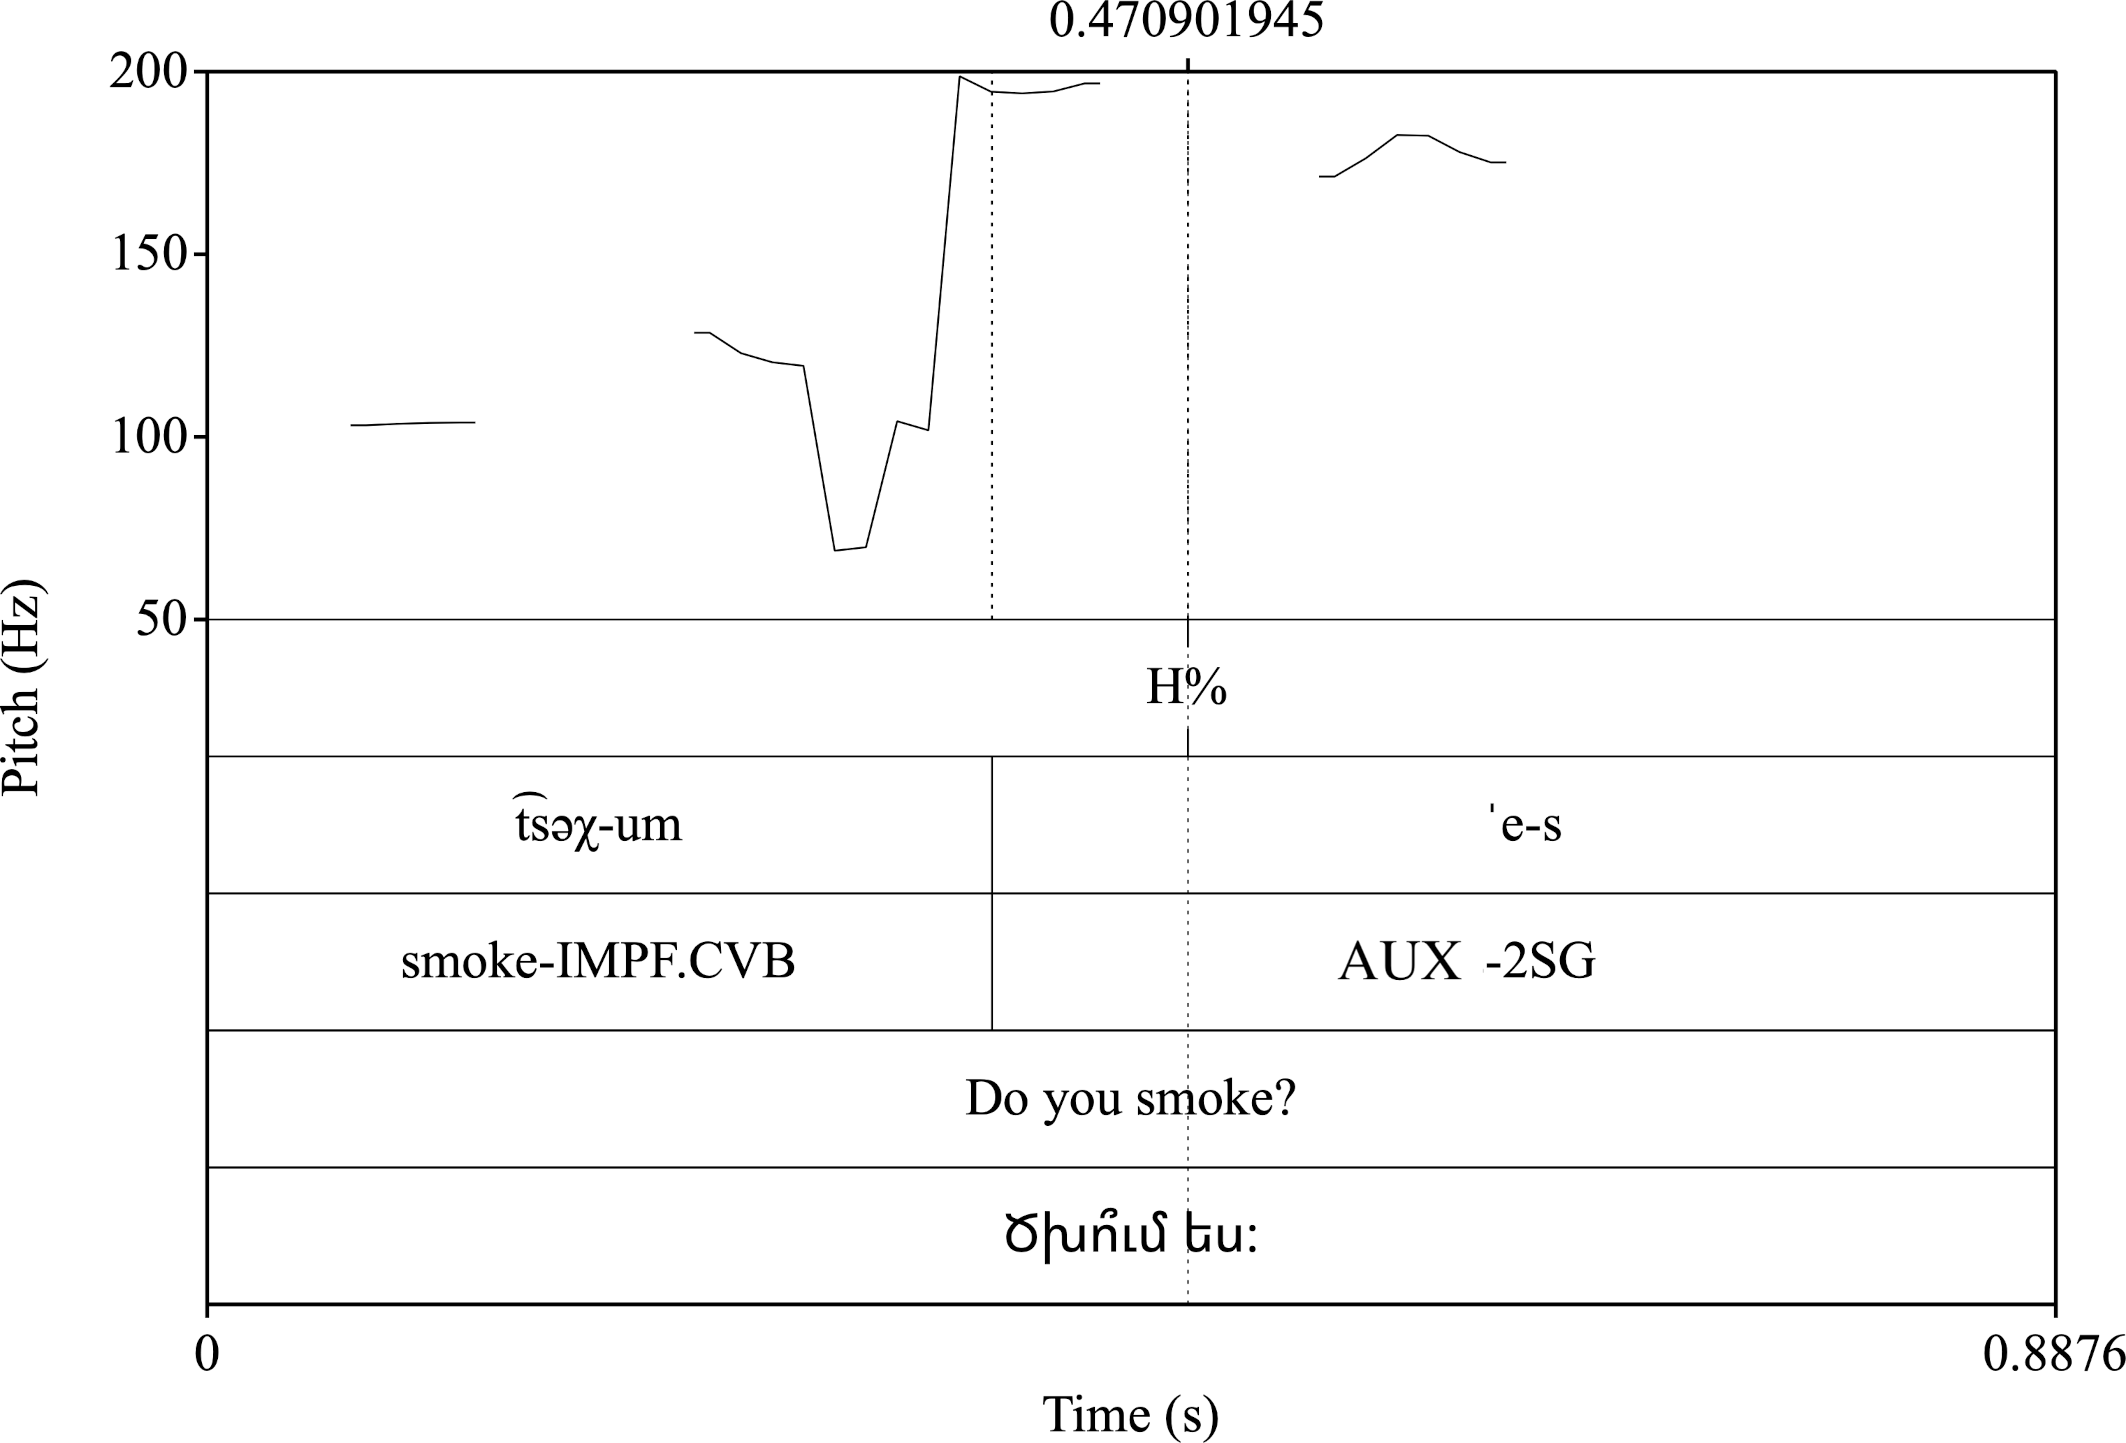
\includegraphics[width=\linewidth]{images/NK_PolarQuestion_Clitic.png}
				\caption{{\iaAbbre} polar  with H\%}
			\end{subfigure}
		\end{figure}
		
		
		
		Such lengthening and rising are also found in wh-questions (\ref{example: wh sentence}). In a subject wh-question in the present tense, the subject is replaced by the wh-word, takes nuclear stress, and is cliticized with the inflected auxiliary. There is a significant rise on the wh-word. The sentence ends with a falling intonation in  {\seaSE} \citep[15]{Johnson-1954-EastArmGrammar}. For {\iaIA}, the sentence can end  in a falling intonation in casual speech.   However, speakers can also  apply a sentence-final rise in order to indicate a degree of politeness.
		

		
		\begin{exe}
			\ex \textit{Subject wh-question}\label{example: wh sentence}
			
			\begin{tabular}{llllll}
				a.& {\uline{ov}}$\nearrow$&={e}& {{ɡiɾkʰ}}& {kɑɾtʰ-um}$\searrow$&({\seaAbbre})
				\\
				& \multicolumn{5}{l }{\armenian{Ո՞վ է գիրք կարդում։}}\\
				b. & {\uline{ov}}$\nearrow$&={ɒ}&   {{ɡiɻkʰ}} & {kɒɻtʰ-um}$\searrow$&({\iaAbbre} - Casual)
				\\
				c. & {\uline{ov}}$\nearrow$&={ɒ}&   {{ɡiɻkʰ}} & {kɒɻtʰ-um}$\nearrow$&({\iaAbbre} - Polite)
				\\
				& who&={\auxgloss}&book& read-{\impfcvb} & 
				\\
				&\multicolumn{4}{l}{`Who is   reading  books?'
				} & 
				\\
				& \multicolumn{5}{l }{\armenian{Ո՞վ  ա գիրք կարդում։}} \\
				
			\end{tabular} 
			
		\end{exe}
		
		Figure \ref{fig:wh iranian low high} (page \pageref{fig:wh iranian low high}) shows the recordings for the above wh-question, one with a final fall L\%, and one with a final rise H\%.  Data is from NK. She at first produced the falling sentence, but in subsequent elicitations preferred the rising sentence.\largerpage[-1]
		
		
		
		
		\begin{figure}
			\caption{Pitch track of wh-question from (\ref{example: wh sentence}) with a final fall (\ref{example: wh sentence}a,b) or with a final rise  (\ref{example: wh sentence}c)  in {\seaSE} and {\iaIA}\label{fig:wh iranian low high}}
			\begin{subfigure}[b]{0.5\textwidth}
				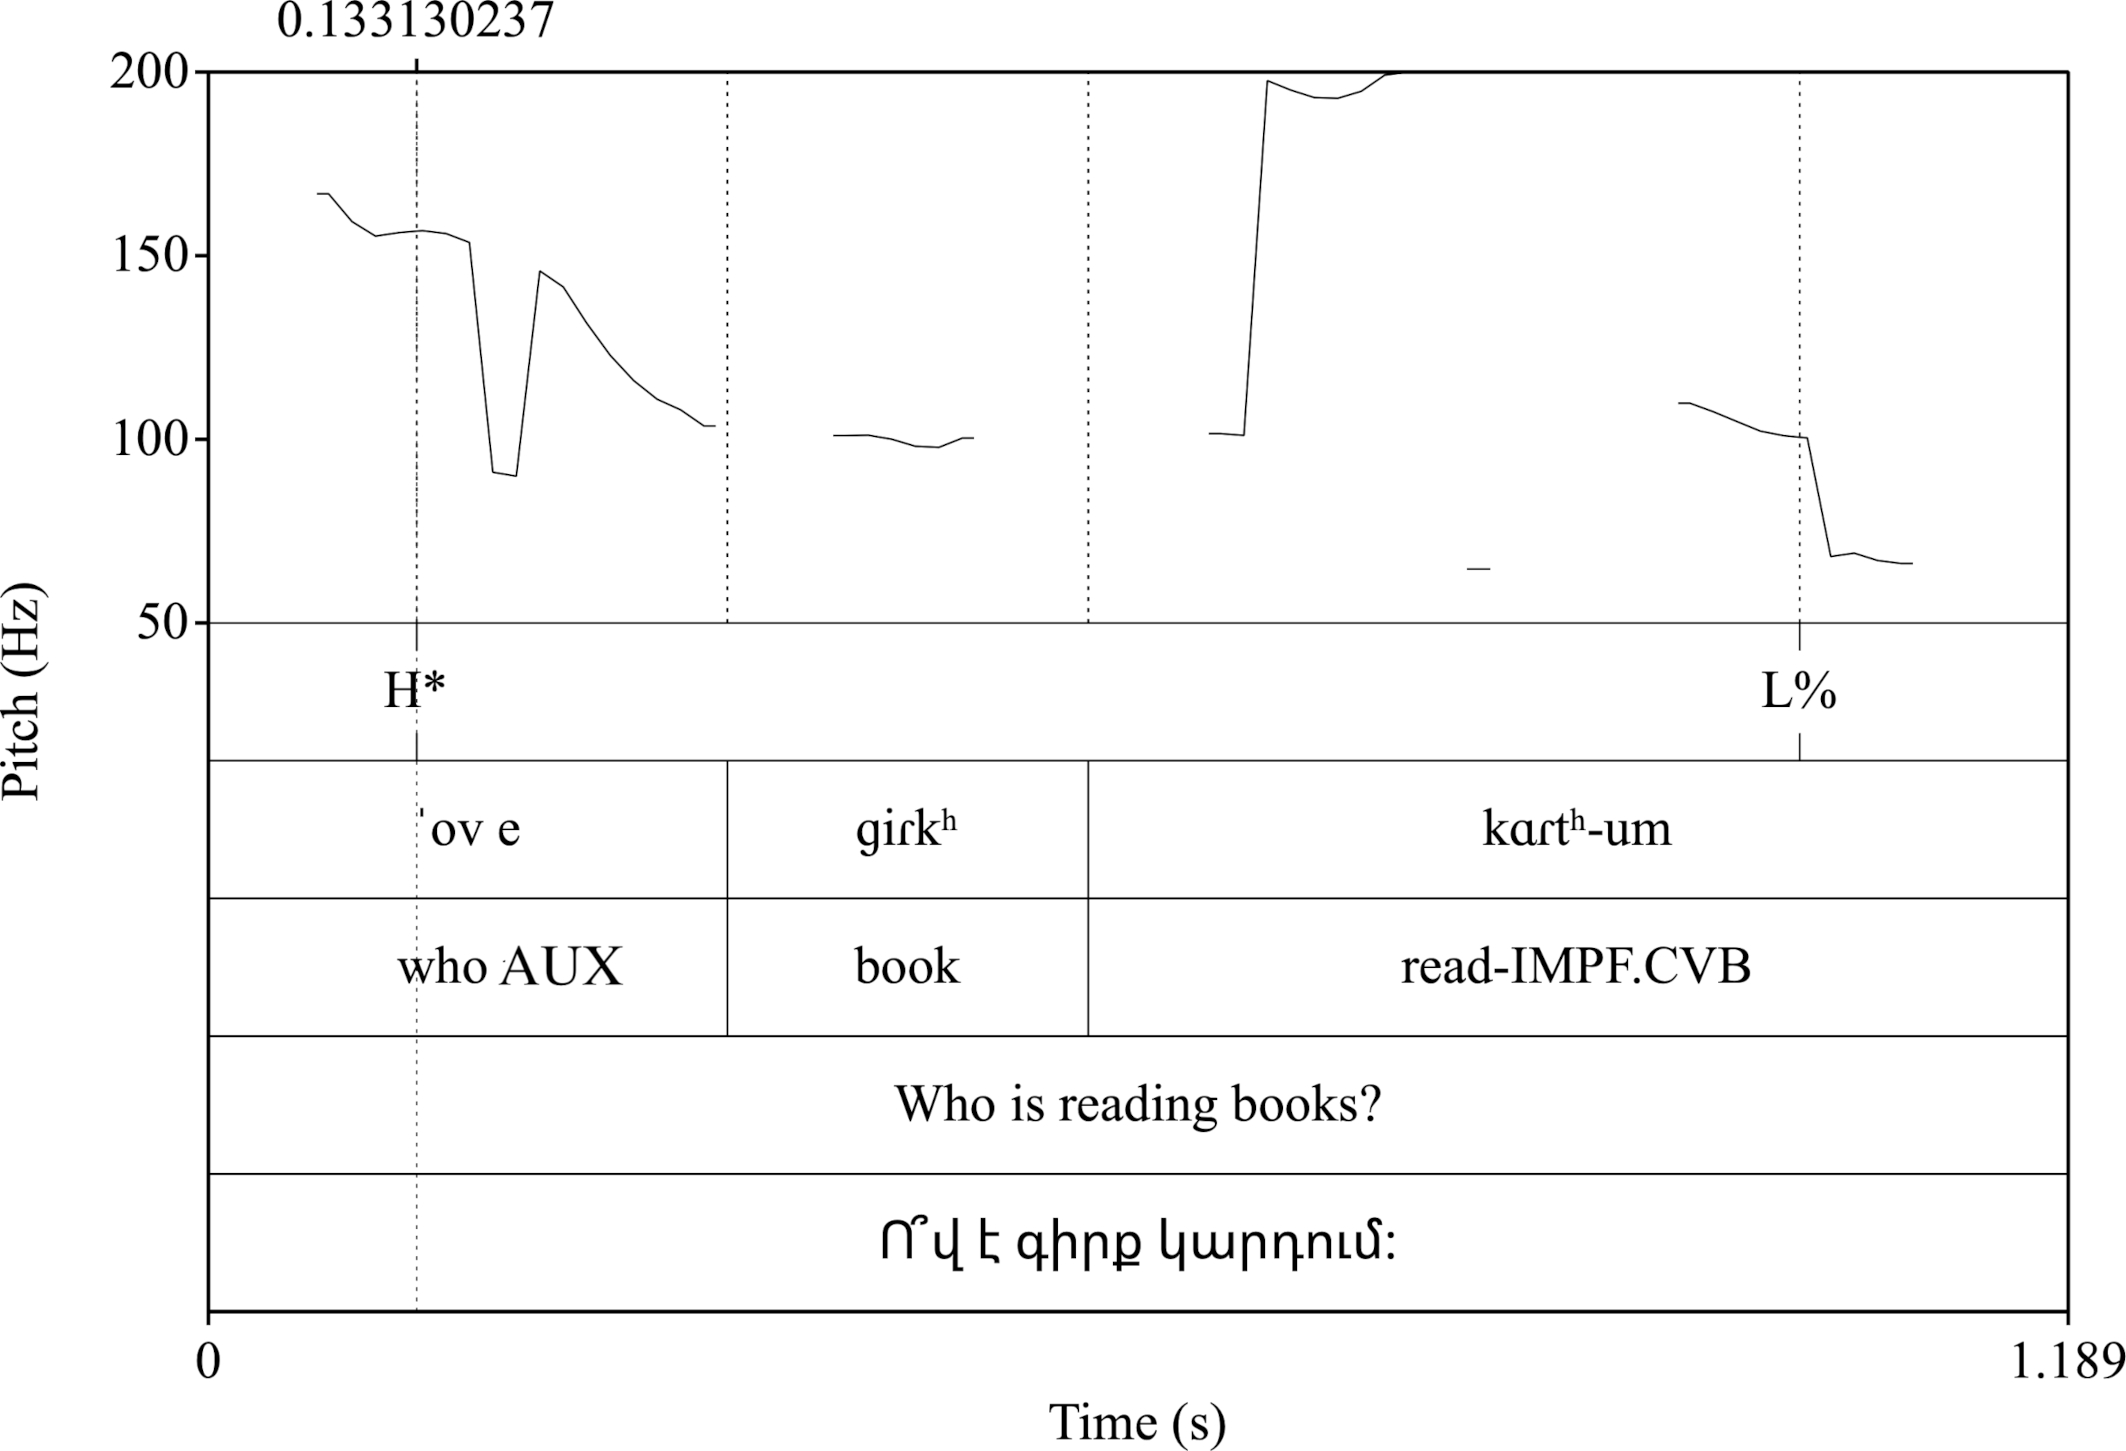
\includegraphics[width=\linewidth]{images/AT_WhQuestion.png}
				\caption{{\seaAbbre} wh-question with L\%}
			\end{subfigure}%
			\begin{subfigure}[b]{0.5\textwidth}
				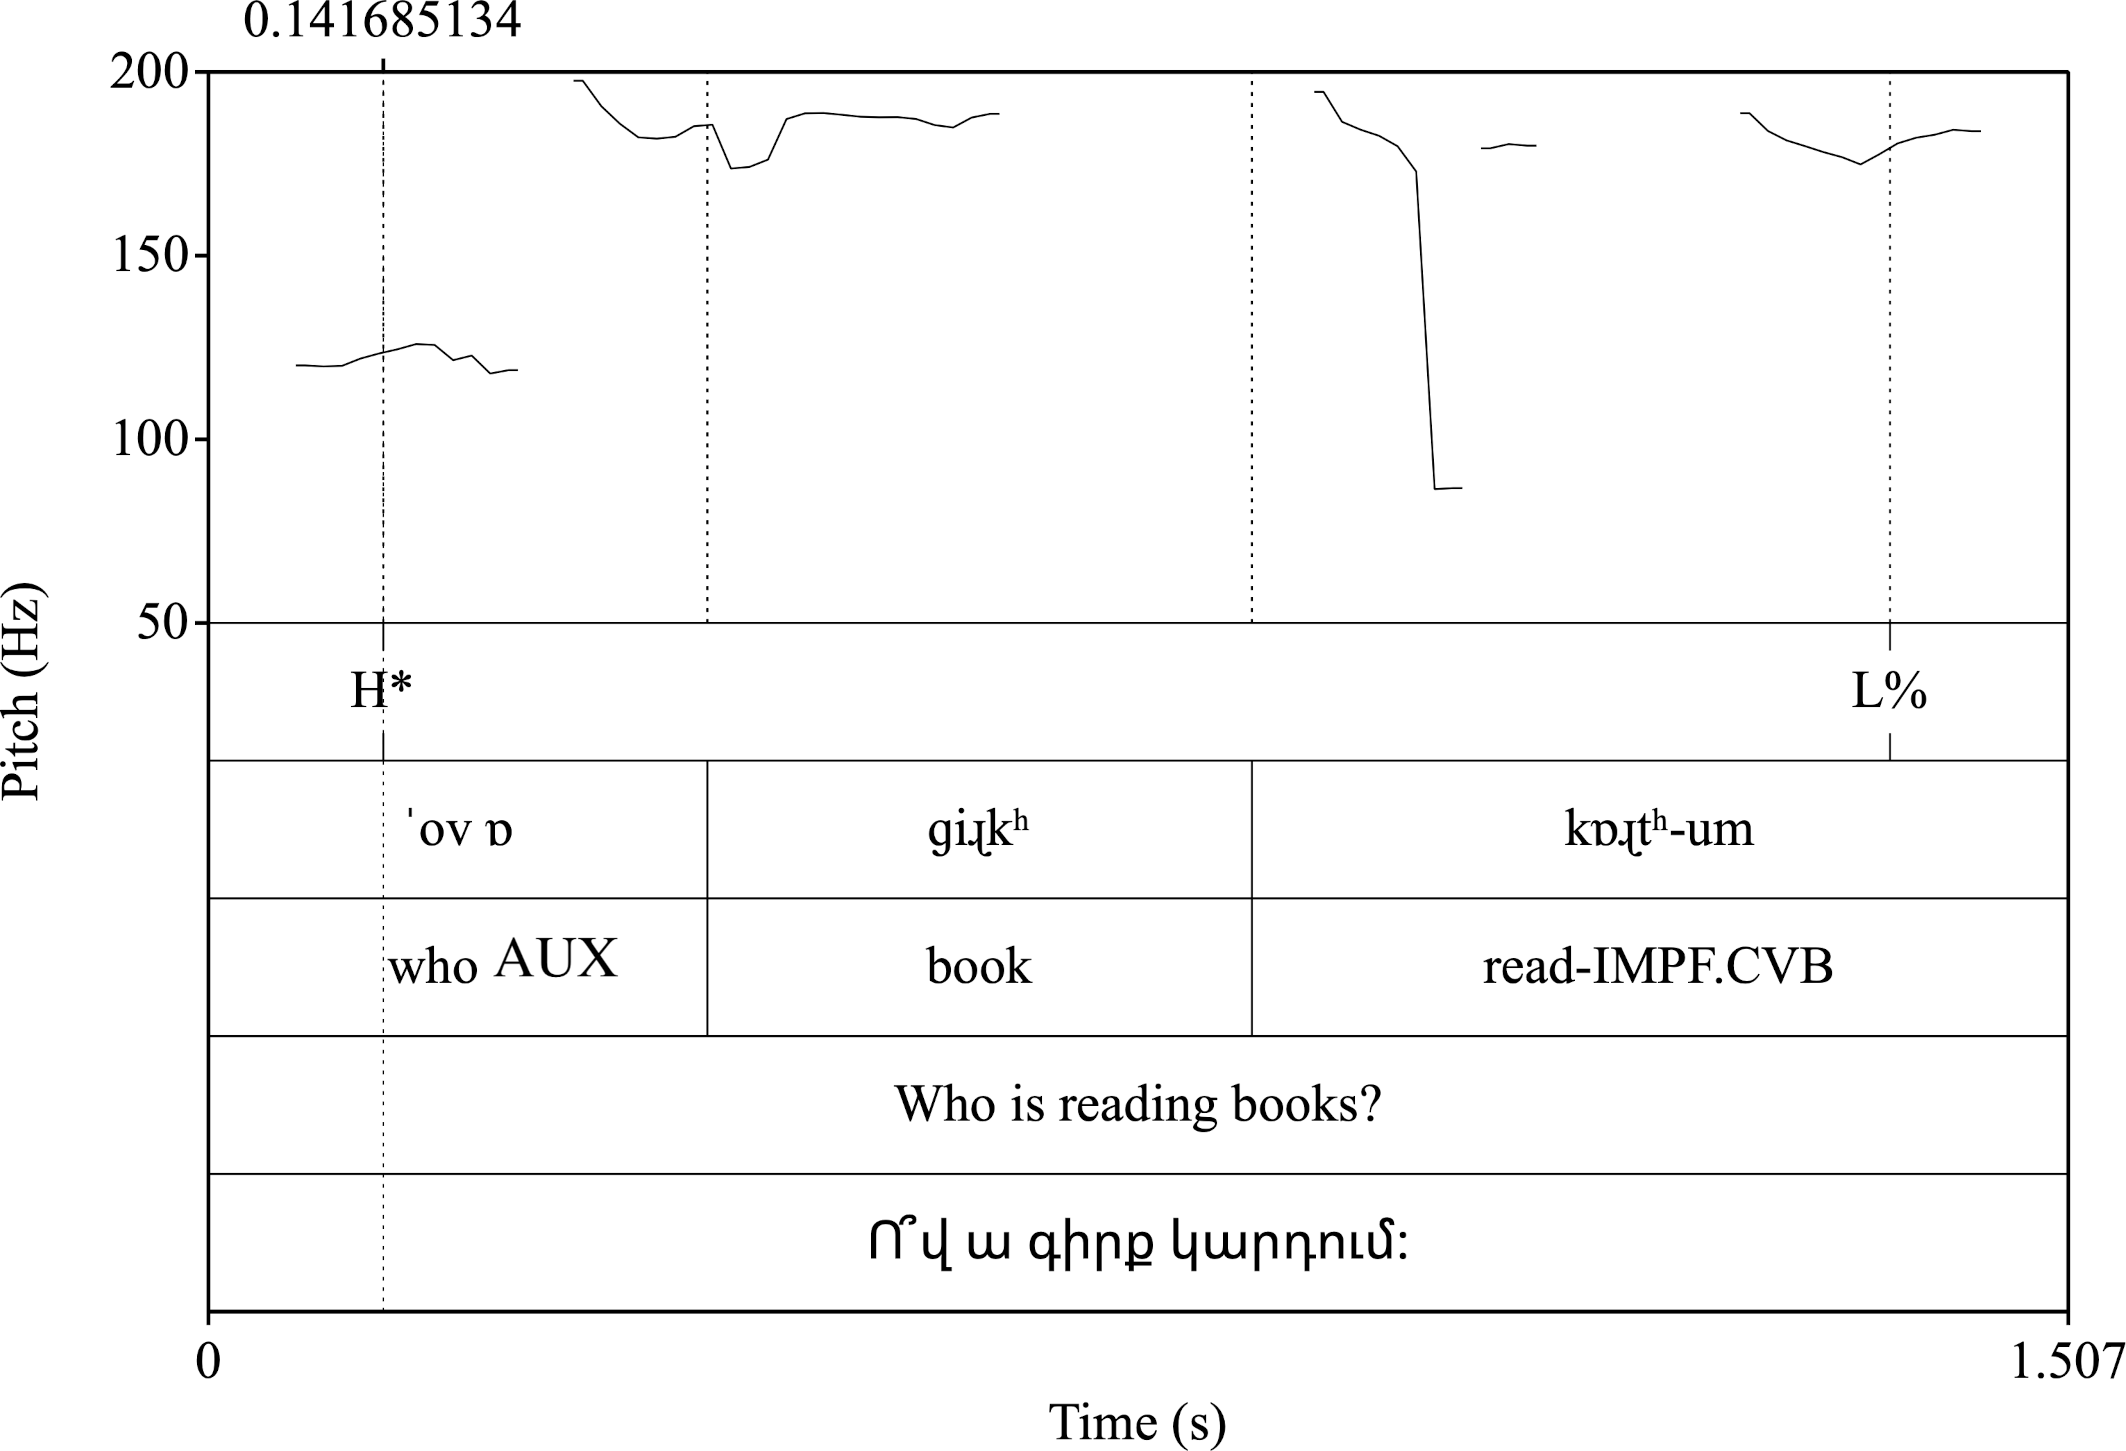
\includegraphics[width=\linewidth]{images/NK_WhQuestion_LowTone.png}
				\caption{{\iaAbbre} wh-question with L\%}
			\end{subfigure}\smallskip\\
			\begin{subfigure}[b]{0.5\textwidth}
				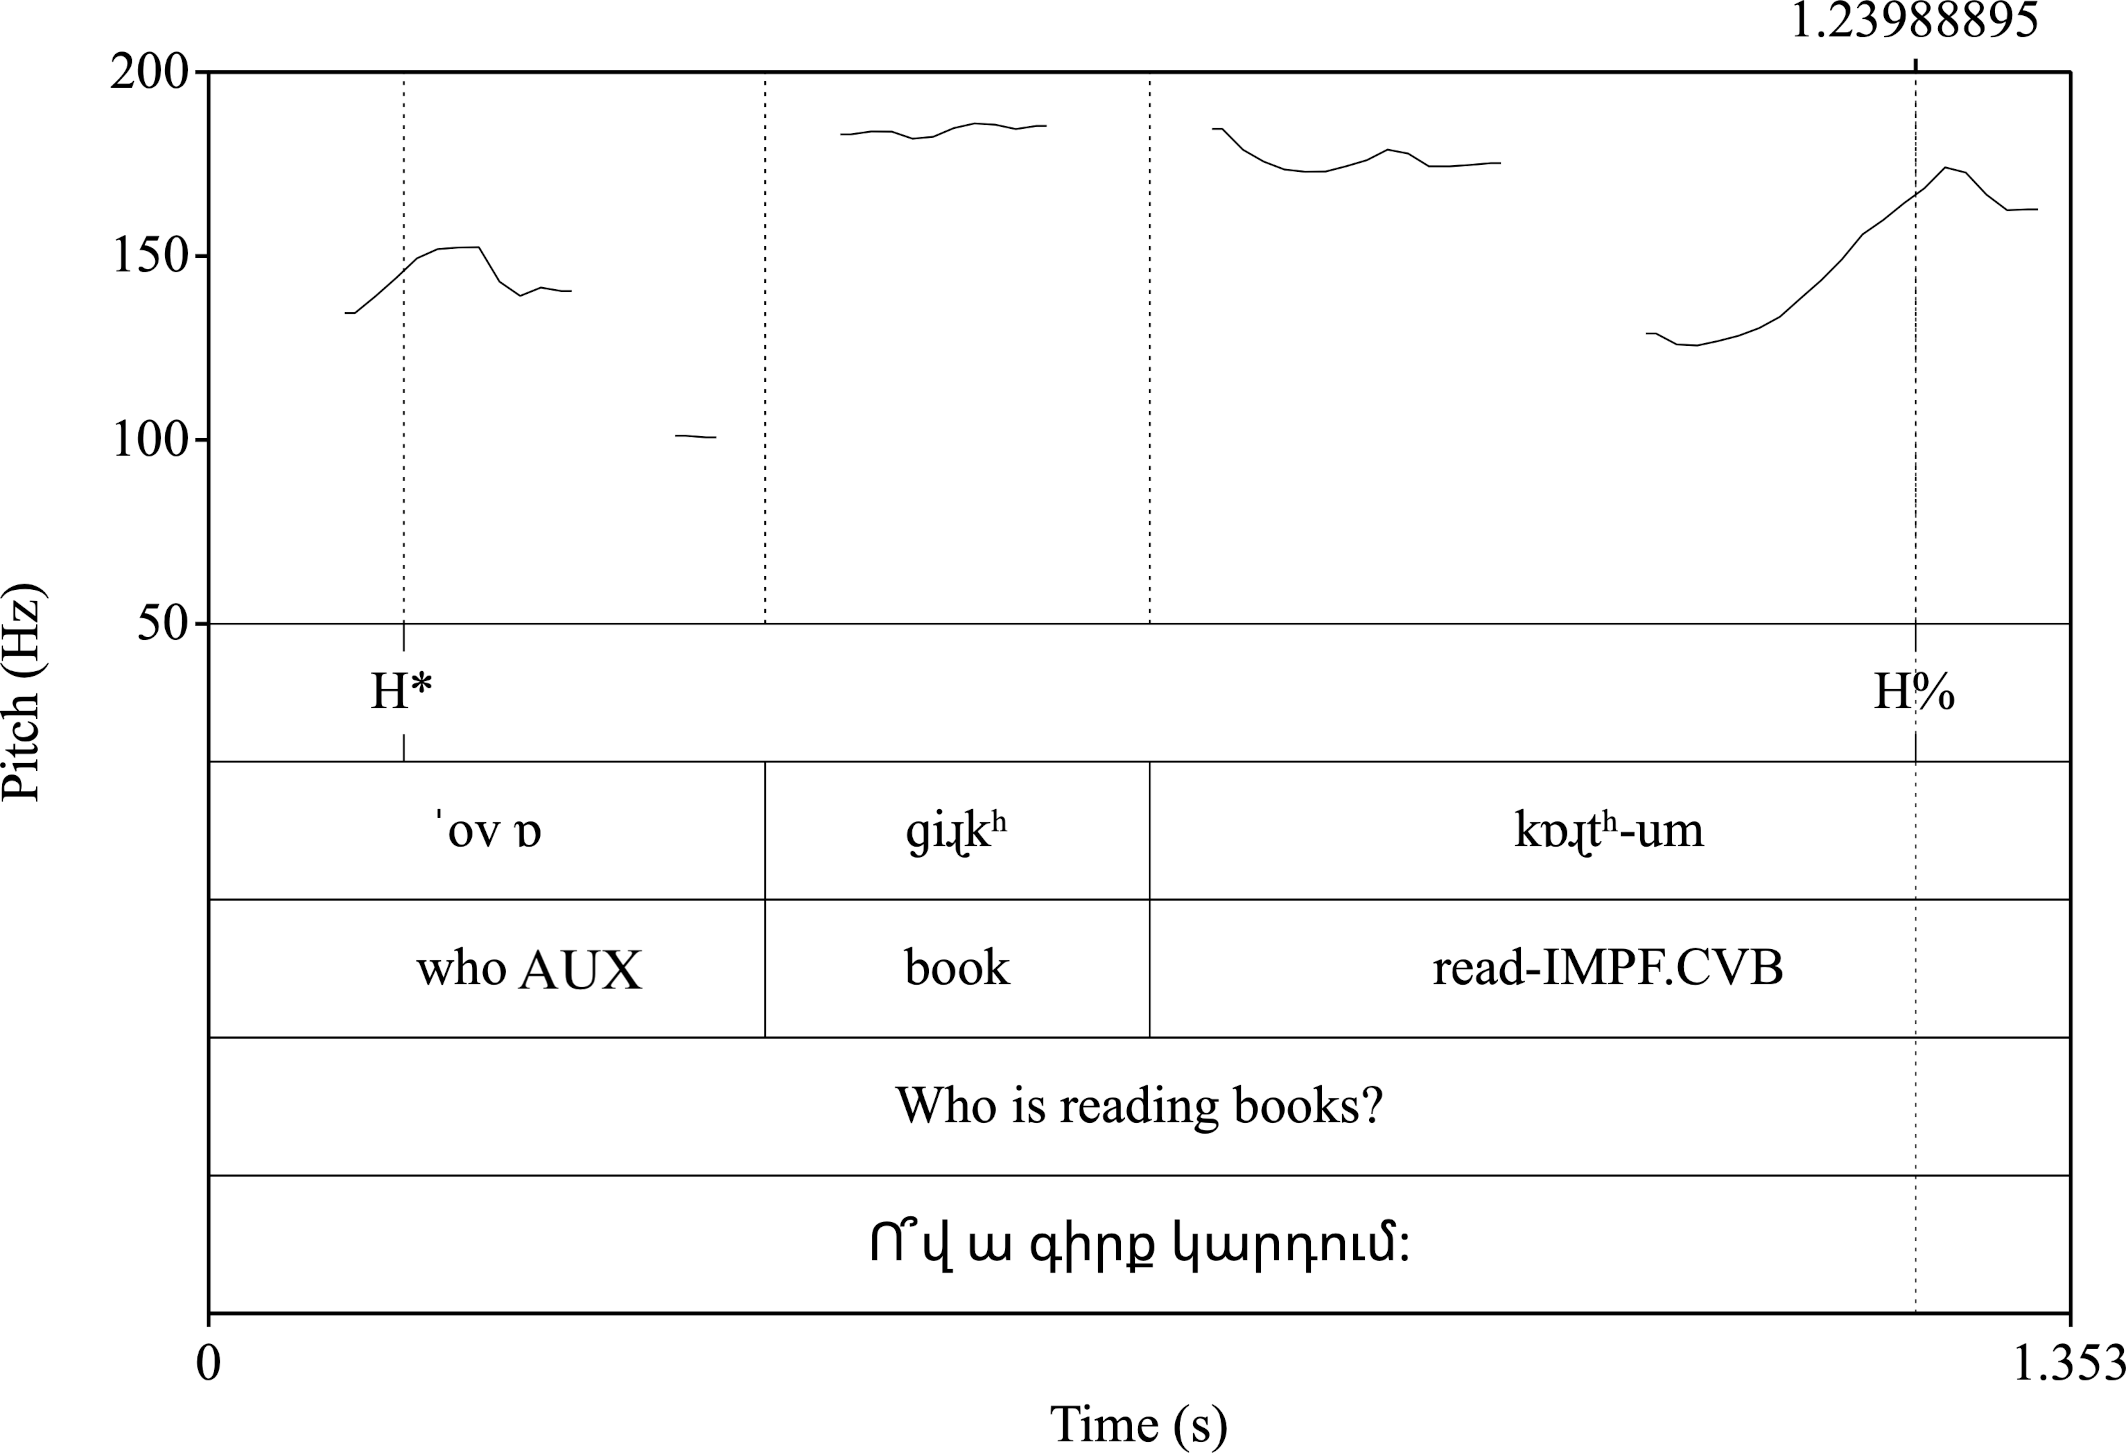
\includegraphics[width=\linewidth]{images/NK_WhQuestion_HighTone.png}
				\caption{{\iaAbbre} wh-question with H\%}
			\end{subfigure}			
		\end{figure}
		
		In Persian, wh-questions likewise end in falling intonation \citep[118]{sadat-2011-intonationPatternsInterrogativesPersian}. Such questions can undergo a final rise and lengthening in order to indicate politeness, curiosity, or a sense of not asserting the question (Sadat-Tehrani, p.c.).  The use of a final rise in wh-questions seems to have become somewhat conventionalized in {\iaIA}. For example, NK produced some wh-questions with     final rises, and some wh-questions with final falls. But she more often used final rises than final falls.   More data is however needed to establish the frequency of using sentence-final rises vs. falls in wh-questions across multiple speakers. 
		
		Finally, recall that {\seaSEA} is used by the Armenian community in Iran as a formal register. It is possible that a contributing factor to the intonational difference between {\seaSE} and {\iaIA} is the fact that Persian utilizes lower pitch in formal contexts \citep{falahati-2020-acquisitionSegmentalSuprasegmentalFeaturesSecondLanguagePersianPoliteness}. Thus, {\iaIA} might have conventionalized the use of sentence-final rises in order to further reinforce the sociolinguistic distinction between formal {\seaSE} and informal {\iaIA}.  
		
		
		In sum, {\iaIA} has adopted aspects of Persian intonation. Such aspects are not due to code switching. It seems that in general, {\iaIA} speakers born in the diaspora (like NK)   do not acquire Persian at the home. 
